\documentclass[]{article}
\PassOptionsToPackage{numbers,compress}{natbib}
\usepackage{jmlr2e}
\usepackage{url}
\usepackage{amsmath}
\usepackage{amssymb}
\usepackage{amsbsy}
\usepackage{siunitx}
\usepackage{algorithm}
\usepackage{algorithmicx}
\usepackage{algpseudocode}
\usepackage{mathtools}
\usepackage{array}
\usepackage{setspace}
%\usepackage{caption}
\usepackage{subcaption}
\usepackage{booktabs}
\usepackage{adjustbox}
\usepackage{microtype}

\usepackage{times}
\usepackage{footmisc}
\usepackage{listings}
\usepackage{color}
\usepackage{xcolor}
\usepackage{textcomp}
\usepackage{xspace}

\usepackage{fancyhdr}


\usepackage{bibentry}
\nobibliography*

\usepackage{paralist}

\usepackage{natbib}
%\bibliographystyle{abbrvnat-simple}
%\setlength{\bibsep}{2.0pt}
%
%\setlength{\floatsep}{5pt plus 2pt minus 2pt}
%\setlength{\textfloatsep}{5pt plus 2pt minus 2pt}
%\setlength{\intextsep}{5pt plus 2pt minus 2pt}

\usepackage{enumitem}
\setlist[itemize]{leftmargin=*}

\usepackage{hyperref}

%\graphicspath{{./figures/}}

\definecolor{darkgreen}{rgb}{0.25,.5,0}
\definecolor{blue}{rgb}{0,0.33,0.66}
\definecolor{red}{rgb}{0.66,0.0,0.0}
\definecolor{purple}{rgb}{0.33,0,0.66}
\definecolor{cyan}{rgb}{0.0,0.5,0.5}
\definecolor{orange}{rgb}{0.5,0.25,0.0}
\definecolor{gray}{rgb}{0.4,0.4,0.4}
\lstset{ 
	language=Lisp, 
	basicstyle=\small\ttfamily,
	keywordstyle={}, 
	alsoletter={/},
	alsoletter={:},
	alsoletter={*},
	alsoletter={<-},
	commentstyle=\em \color{gray}, 
	frame=lines,
	%float=tbph,
	% captionpos=b,
	showstringspaces=false, 
	keywordstyle=[1]\bf\ttfamily\color{blue},
	keywords=[1]{BO,theta-best,bo-acquire,sample-initial-points,sample,observe,observe*,observe<-,predict,store,retrieve,return,catch,throw},
	keywordstyle=[2]\bf\ttfamily\color{red},
	keywords=[2]{defn,if,let,letfn,loop,looppredict,recur},
	keywordstyle=[3]\bf\ttfamily\color{cyan},
	keywords=[3]{absorb,assoc,argmax,count,cons,conj,dirichlet-discrete,do,exponential,first,flip,fn,gamma,beta,get,keys,lazy-seq,map,mvn-niw,nth,mat/add,mat/div,normal,print,produce,reduce,repeat,repeatedly,rest,set,shape,take,uniform-continuous,vec,distribution,factor,simulate,abc-likelihood,when,max},
	keywordstyle=[4]\bf\ttfamily\color{purple},
	keywords=[4]{defopt,defquery,doopt,doquery,query,defdist},
	keywordstyle=[5]\ttfamily\color{orange},
	keywords=[5]{:nu,:alpha,:id},
	mathescape=true,
	stringstyle={},
} 
\lstnewenvironment{code}[2]{\lstset{caption=#1,label=#2}}{}

\newcommand{\lsi}[1]{\lstinline$#1$}

\newcommand{\sample}{\lstinline$sample$\xspace}
\newcommand{\observe}{\lstinline$observe$\xspace}
\newcommand{\observes}{\lstinline$observe<-$\xspace}
\newcommand{\predict}{\lstinline$predict$\xspace}
\newcommand{\simulatec}{\lstinline$simulate$\xspace}
\newcommand{\abcl}{\lstinline$abc-likelihood$\xspace}
\newcommand{\factor}{\lstinline$factor$\xspace}

\newcommand{\defdist}{\lstinline$defdist$\xspace}
\newcommand{\defquery}{\lstinline$defquery$\xspace}
\newcommand{\query}{\lstinline$query$\xspace}
\newcommand{\defopt}{\lstinline$defopt$\xspace}
\newcommand{\doquery}{\lstinline$doquery$\xspace}
\newcommand{\doopt}{\lstinline$doopt$\xspace}
\newcommand{\normal}{\lstinline$normal$\xspace}
\newcommand{\betaa}{\lstinline$beta$\xspace}
\newcommand{\gammaa}{\lstinline$gamma$\xspace}

%\newcommand{\observe}{\texttt{\small\bf\color{darkgreen} observe}\xspace}
%\newcommand{\predict}{\texttt{\small\bf\color{darkgreen} predict}\xspace}
%\newcommand{\sample}{\texttt{\small\bf\color{darkgreen} sample}\xspace}
%\newcommand{\defquery}{\texttt{\small\bf\color{darkgreen} defquery}\xspace}
%\newcommand{\normal}{\texttt{\small\bf\color{blue} normal}\xspace}
%\newcommand{\boaq}{\texttt{\small\bf\color{blue} bo-acquire}\xspace}
%\newcommand{\sampleinitpoints}{\texttt{\small\bf\color{blue} sample-initial-points}\xspace}

%\newcommand{\defopt}{\texttt{\small\bf\color{darkgreen} defopt}\xspace}
%\newcommand{\doopt}{\texttt{\small\bf\color{darkgreen} doopt}\xspace}
%\newcommand{\doquery}{\texttt{\small\bf\color{darkgreen} doquery}\xspace}
%\newcommand{\defdist}{\texttt{\small\bf\color{darkgreen} defdist}\xspace}

%\usepackage{wrapfig,lipsum,booktabs}

%\usepackage{hyperref}


\newcolumntype{A}{>{\centering\arraybackslash}m{1cm}}

\newcolumntype{B}{>{\centering\arraybackslash}m{1.5cm}}

\newcolumntype{D}{>{\centering\arraybackslash}m{2cm}}

\renewcommand*\Call[2]{\textproc{#1}(#2)}

\algnewcommand{\IIf}[1]{\unskip \algorithmicif\ #1\ \algorithmicthen}
\algnewcommand{\ElseIIf}{\unskip\ \algorithmicelse}
\algnewcommand{\EndIIf}{\unskip\ \algorithmicend\ \algorithmicif}

\newcommand{\mX}{\mathcal{X}}
\newcommand{\mD}{\mathcal{D}}
\newcommand{\nx}{_{\mathrm{next}}}
\newcommand{\real}{\mathbb{R}}
\newcommand{\xpos}{\tilde{\mathbf{x}}}
\newcommand{\xb}{\mathbf{x}}
\newcommand{\yb}{\mathbf{y}}
\newcommand{\zb}{\mathbf{z}}
\newcommand{\hb}{\mathbf{h}}
\newcommand{\hx}{h\left(\xb,\zb\right)}

\newcommand{\hu}{\hat{u}}
\newcommand{\hz}{\hat{Z}}
\newcommand{\hw}{\hat{w}}
\newcommand{\hth}{\hat{\theta}}
\newcommand{\ho}{\hat{\Omega}}

\newcommand{\tilz}{\tilde{Z}}
\newcommand{\tilw}{\tilde{w}}
\newcommand{\tilth}{\tilde{\theta}}
\newcommand{\tilo}{\tilde{\Omega}}

\newcommand{\jsm}{j^*_m}

\newcommand{\bc}{\left(\cdot\right)}
\newcommand{\bcc}{\left(\cdot\right)}
\newcommand{\mM}{\mathcal{M}}
\newcommand{\tx}{\texttt{x}}
\newcommand{\ty}{\texttt{y}}
\newcommand{\tz}{\texttt{z}}
\newcommand{\tb}{\texttt{b}}
\newcommand{\ft}{f\left(\theta\right)}
\newcommand{\tth}{\tilde{\theta}}
\newcommand{\mut}{\mu_m\left(\theta ; \alpha\right)}
\newcommand{\kt}{k_{m}\left(\theta,\theta'\right)}
\newcommand{\sut}{\sigma_m\left(\theta ; \alpha\right)}
\newcommand{\gut}{\gamma_{m}\left(\theta\right)}

\newcommand{\RN}[1]{%
	\textup{\uppercase\expandafter{\romannumeral#1}}%
}
\renewcommand{\v}[1]{\ensuremath{\boldsymbol{#1}}}

\DeclareMathOperator*{\argmax}{arg\,\!max}
\DeclareMathOperator{\Normal}{Normal}
\DeclareMathOperator{\Dirichlet}{Dirichlet}
\DeclareMathOperator{\Gammaa}{Gamma}
\DeclareMathOperator{\simulate}{simulate}
\DeclareMathOperator{\dist}{dist}
\DeclareMathOperator{\std}{std}


\newcommand{\qmarg}{\texttt{q-marg}}
\newcommand{\qprior}{\texttt{q-prior}}
\newcommand{\qacq}{\texttt{q-acq}}


\ShortHeadings{Bayesian Optimization for Probabilistic Programs}{Rainforth, Le, van de Meent, Osborne and Wood}
\firstpageno{1}

\title{Bayesian Optimization for Probabilistic Programs$^*$}

\author{\name Tom Rainforth \email twgr@robots.ox.ac.uk \\
	\addr Department of Engineering Science, University of Oxford
	\AND
	\name Tuan Anh Le \email tuananh@robots.ox.ac.uk \\
	\addr Department of Engineering Science, University of Oxford
	\AND
	\name Jan-Willem van de Meent \email j.vandemeent@northeastern.edu \\
	\addr College of Computer and Information Science, Northeastern University
	\AND
	\name Michael A Osborne \email mosb@robots.ox.ac.uk \\
	\addr Department of Engineering Science, University of Oxford
	\AND
	\name Frank Wood \email fwood@robots.ox.ac.uk \\
	\addr Department of Engineering Science, University of Oxford \\
}

\fancypagestyle{empty}{%
	\fancyhf{}% Clear header/footer
	\fancyhead[L]{}% Your journal/note
	\renewcommand{\headrulewidth}{0pt}
	\renewcommand{\footrulewidth}{0pt}
	\fancyfoot[L]{\footnotesize \vspace{-25pt} \rule{\textwidth}{0.4pt} \indent{} \indent{} *Please cite this version: \\ \vspace{5pt} \hspace{20pt} \begin{minipage}{0.9\textwidth}\bibentry{rainforth2016bayesian}\end{minipage}}% Your logo/image
}

\begin{document}
%
%\input{coverArXiv.tex}
%\newpage

\maketitle
\vspace{-30pt}

\newcommand\blfootnote[1]{%
	\begingroup
	\renewcommand\thefootnote{}\footnote{#1}%
	\addtocounter{footnote}{-1}%
	\endgroup
}

\begin{abstract}
% !TEX root =  ../main.tex

So far in this thesis, and in the literature more generally, the focus has been on automating
inference for probabilistic programs.  However, as we explained in Section~\ref{sec:opt:intro},
optimization is also a very important tool in the machine learning toolbox.  Further, many problems
require concurrent inference and optimization in the form of marginal maximum a posteriori (MMAP) estimation,
maximum marginal likelihood (MML) estimation, or risk minimization.  In this chapter, we develop a probabilistic programming framework
for automating the solution of these mixed inference-optimization problems.
We will focus for the most part on
MMAP estimation, highlighting differences for MML estimation and risk minimization when necessary.

MMAP estimation is challenging as it corresponds to the optimization of an intractable integral, such that the 
optimization target is expensive to evaluate and gives noisy results.  Current PPS inference engines are 
typically unsuited to such settings.  We therefore introduce BOPP\footnote{Code available at \url{http://www.github.com/probprog/bopp/}}
(Bayesian optimization for probabilistic programs)~\citep{rainforth2015workshopbopp,rainforth2016bayesian}, 
which uses a series of code transformations, existing inference algorithms,
and a bespoke Gaussian process (GP) based Bayesian optimization (BO) package, which we call Deodorant\footnote{Code available
at \url{http://www.github.com/probprog/deodorant/}}, to optimize the evidence of a query with respect to
an arbitrary subset of its internally sampled variables.\footnote{As we will explain later, there is no need to
	provide separate consideration for optimizing with respect to the inputs of the query as, if required,
	variables can be trivially internalized.}

BOPP can be viewed from two different perspectives, providing distinct contributions to both the probabilistic
programming and Bayesian optimization literatures.  From a probabilistic programming perspective, we can
view BOPP as extending PPSs beyond their typical inference setting to a more
general mixed inference-optimization framework.  It allows users to specify a model in the same manner 
as existing systems, but then select some subset of the sampled variables in the query to be optimized, 
with the rest marginalized out using existing inference algorithms.  Though the exact code transformations we
introduce are inevitably language specific and have been implemented for Anglican, the concepts we
introduce apply more widely and the BO package itself, Deodorant, is not PPL specific and is provided
as a stand-alone package.  More generally, the \textit{optimization query} we 
introduce can be implemented and utilized in any PPL that supports an inference method returning a 
partition function estimate.  This framework increases the scope of models that can be expressed in
PPSs and gives additional flexibility in the outputs a user can request from a program.

From a BO perspective, we can view BOPP as the first package to directly exploit the source code of its target.
This leads to a number of novel contributions to the BO literature, such as innovations in 
problem-independent hyperpriors, unbounded optimization, and implicit constraint satisfaction.  
The ability to do these is rooted
in the ability provided by PPLs to manipulate the target source code and return artifacts suitable for carrying
out certain tasks on a model.  For example, we use a code transformation to produce a problem-specific
optimizer for the acquisition function that ensures the implicit constraints specified by the query,
including equality constraints not before considered by the BO literature, are automatically and exactly
satisfied.  As a consequence, BOPP provides a significant novel features and performance
improvements even when used simply as a conventional BO package.
%\blfootnote{\hspace{-20pt}*Please cite this version: \\ \bibentry{rainforth2016bayesian}}
\end{abstract}

\thispagestyle{empty}


\section{Introduction} 
\label{sec:IntroductionBOPP}

% !TEX root =  ../main.tex

\todo[inline]{Move this first paragraph to the prob prog section to make a better opening}

Probabilistic programming systems (PPS) allow probabilistic models to be represented in the form of a generative model and statements for conditioning on data \citep{carpenter2015stan,goodman_uai_2008,goodman_book_2014,mansinghka2014venture,minka_software_2010,wood2014new}.  
%Informally, one can think of the generative model as the definition of a prior, the conditioning statements as the definition of a likelihood and the output of the program as samples from a posterior distribution. 
Their core philosophy is to decouple model specification and inference, the former corresponding to the user-specified program code and the latter to an inference engine capable of operating on arbitrary programs.  Removing the need for users to write inference algorithms significantly reduces the burden of developing new models and makes effective statistical methods accessible to non-experts.
%This inference engine must therefore be general purpose and robust, without making strong assumptions about the structure of the program, often taking the form of a Monte Carlo sampling scheme such as Markov chain Monte Carlo (MCMC) \citep{wingate2011lightweight}, Hamiltonian Monte Carlo \citep{carpenter2015stan}, sequential Monte Carlo (SMC) \citep{wood_aistats_2014} or particle MCMC \citep{van2015particle}.  

Although significant progress has been made on the problem of general purpose \emph{inference} of program variables, less attention has been given to their \emph{optimization}.  Optimization is an essential tool for effective machine learning, necessary when the user requires a single estimate. It also often forms a tractable alternative when full inference is infeasible \citep{murphy2012machine}.  Moreover, coincident optimization and inference is often required, corresponding to a marginal maximum a posteriori (MMAP) setting where one wishes to maximize some variables, while marginalizing out others.  Examples of MMAP problems include hyperparameter optimization, expectation maximization, and policy search \citep{van2015black}.

%Here pure optimization, i.e. assuming the best possible possible environment, is clearly unsatisfactory, whilst inference alone is insufficient to determine the optimal action.

%Although significant progress has been made on the problem of general purpose \emph{inference} of program variables, less attention has been given to their \emph{optimization}. In many machine learning problems one might want to perform marginal maximum a posterior (MMAP) estimation to obtain a point estimate for a subset of random variables in a model while marginalizing over the remaining variables. Examples of such settings include hyperparameter optimization, decision making under uncertainty \cite{van2015black}, and problems where inference over top-level variables is either infeasible or the user simply desires a single point estimate \cite{murphy2012machine}.

%Even when these simulations are deterministic, this is an approximation to a truly probabilistic world. This setting corresponds to a MMAP framework, in which the user wishes to select the best design whilst marginalizing out the uncertainty about the environment or the simulation itself.

%To demonstrate how easily BOPP can be used, we present an application of optimal power allocation is shown in Figure \ref{fig:houses} with associated code in Figure \ref{fig:house-heating-code}.  Typically an engineer might try to solve this problem by making a number of fixed environmental assumptions and invoking a finite element simulation software, tuning by hand.  This process can be laborious and fails to capture the uncertainty in the environment.  BOPP provides a framework to naturally incorporate these uncertainties, whilst still exploiting the original simulation and returning a single solution the engineer can implement.

%In this paper we develop the first system that extends probabilistic program (PP) inference to a more general MMAP framework, wherein the user specifies a model in the same manner as existing systems, but then selects some subset of the sampled variables in the program to be optimized, with the rest marginalized using existing inference algorithms.  To do so, we define an \emph{optimization query}, which performs a program transformation to map unconditioned random variables onto conditioned random variables, whose values are passed to the transformed program as inputs. We then introduce Bayesian optimization for probabilistic programs (BOPP), a new framework for Gaussian process (GP) \citep{rasmussen2006gaussian} based  Bayesian optimization (BO) \citep{osborne2009gaussian, jones1998efficient} package integrated into the PPS Anglican \citep{wood2014new}. The BOPP method iteratively performs inference in a conditioned program using a generic method, such as sequential Monte Carlo (SMC), to obtain an unbiased estimate of the marginal likelihood of a conditioned program. Bayesian optimization of this marginal likelihood is then done by constructing a GP surrogate and maximizing the expected improvement \cite{brochu2010tutorial} to select values in a manner that balances exploration and exploitation. 

In this paper we develop the first system that extends probabilistic programming (PP) to this more general MMAP framework, wherein the user specifies a model in the same manner as existing systems, but then selects some subset of the sampled variables in the program to be optimized, with the rest marginalized out using existing inference algorithms.  The \textit{optimization query} we introduce can be implemented and utilized in any PPS that supports an inference method returning a marginal likelihood estimate.  This framework increases the scope of models that can be expressed in PPS and gives additional flexibility in the outputs a user can request from the program.

MMAP estimation is difficult as it corresponds to the optimization of an intractable integral, such that the optimization target is expensive to evaluate and gives noisy results.  Current PPS inference engines are typically unsuited to such settings.  We therefore introduce BOPP\footnote{Code available at \href{http://www.github.com/probprog/bopp/}{\url{http://www.github.com/probprog/bopp/}} \vspace{7pt}} 
(Bayesian optimization for probabilistic programs) which couples existing inference algorithms from PPS, like \emph{Anglican} \citep{wood2014new}, with a new Gaussian process (GP) \citep{rasmussen2006gaussian} based Bayesian optimization (BO) package \citep{gutmann2016bayesian, jones1998efficient, osborne2009gaussian, shahriari2016unbounded}.  

To demonstrate the functionality provided by BOPP, we consider an example application of engineering design.  Engineering design relies extensively on simulations which typically have two things in common: the desire of the user to find a single best design and an uncertainty in the environment in which the designed component will live. Even when these simulations are deterministic, this is an approximation to a truly stochastic world. By expressing the utility of a particular design-environment combination using an approximate Bayesian computation (ABC) likelihood \citep{csillery2010approximate}, one can pose this as a MMAP problem, optimizing the design while marginalizing out the environmental uncertainty.

\flushbottom

\begin{figure*}[t]
	%\includegraphics[width=\textwidth]{"figures/house-heating/deterministic/house-heating-deterministic-with-convergence"}
	\centering
	\begin{subfigure}[t]{0.47\textwidth}
		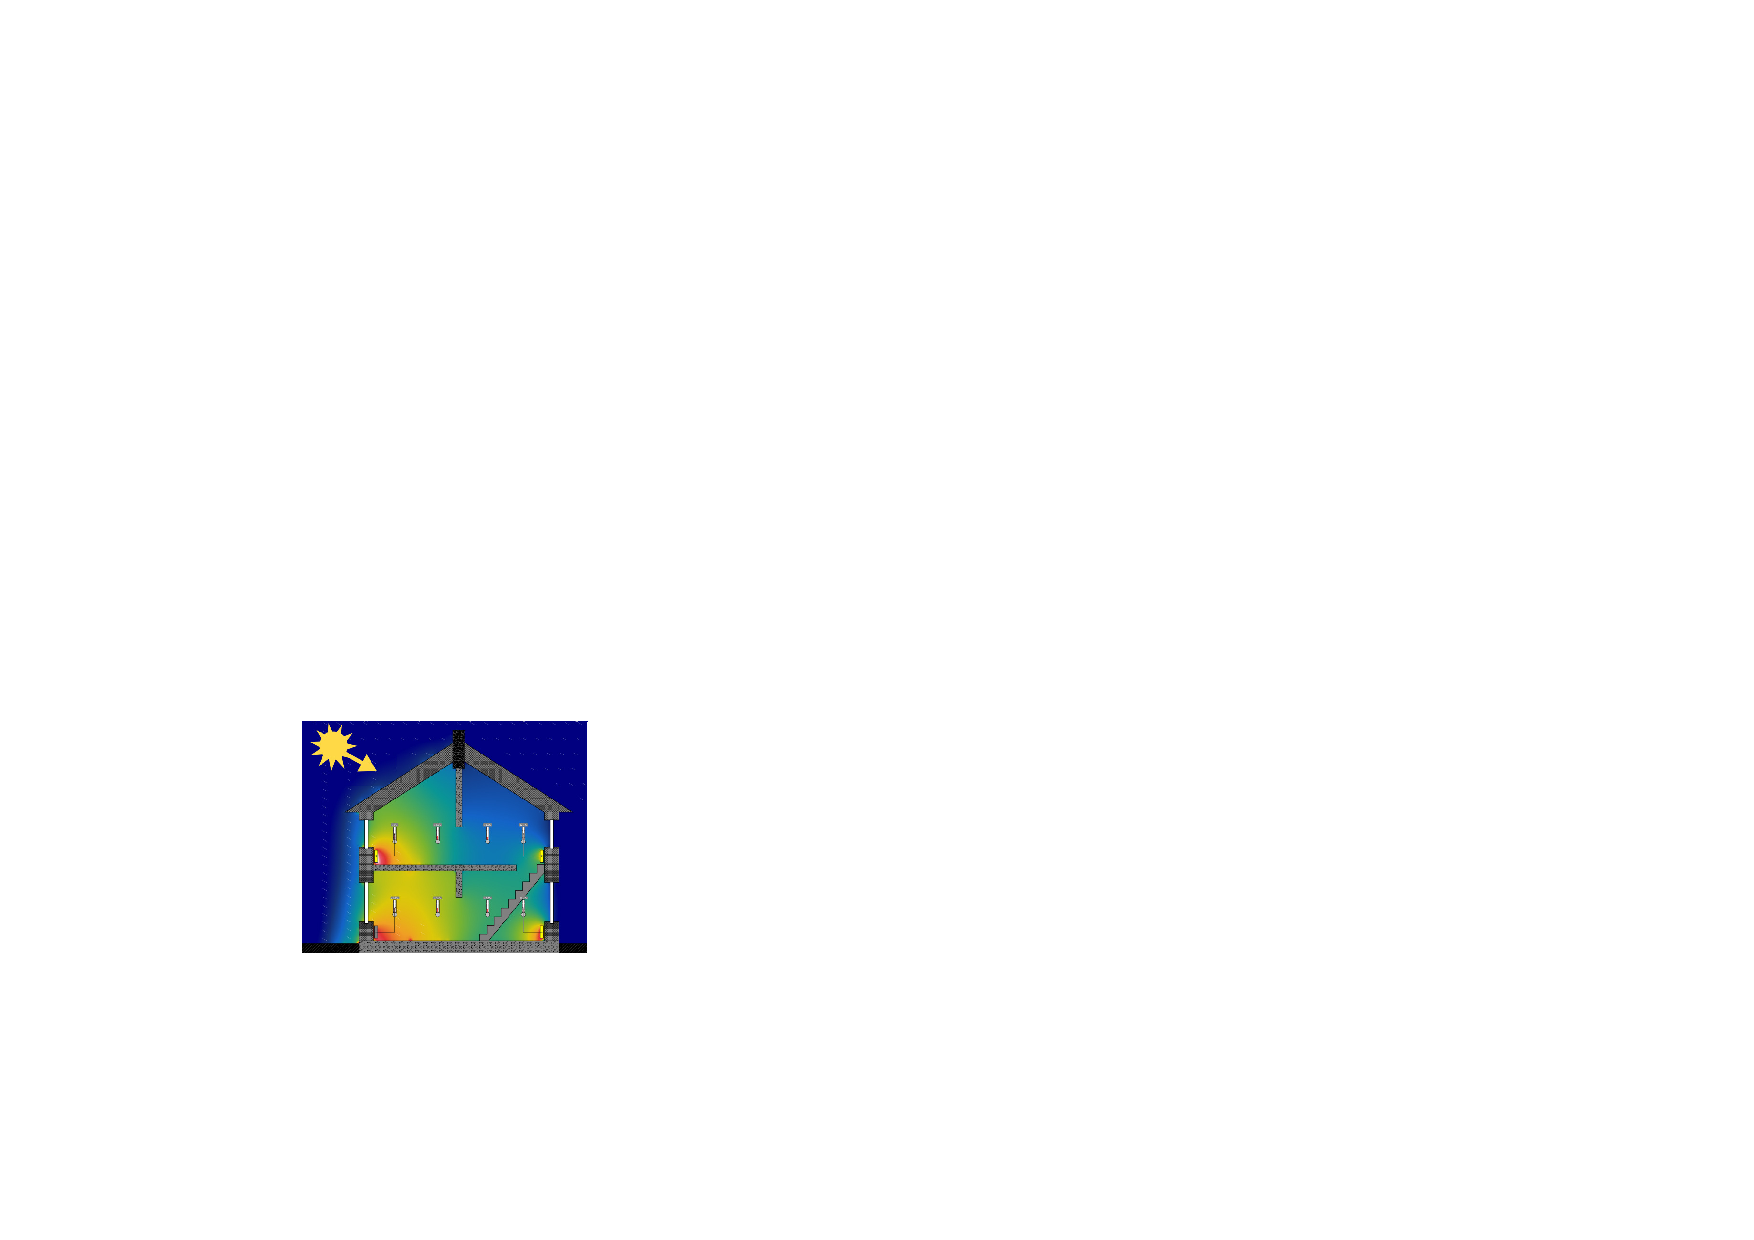
\includegraphics[width=\textwidth]{house-heating/even_powers.pdf}
		\caption{Radiator powers set evenly}
	\end{subfigure}
	~~~~ %\hspace{40pt}
		\begin{subfigure}[t]{0.47\textwidth}
			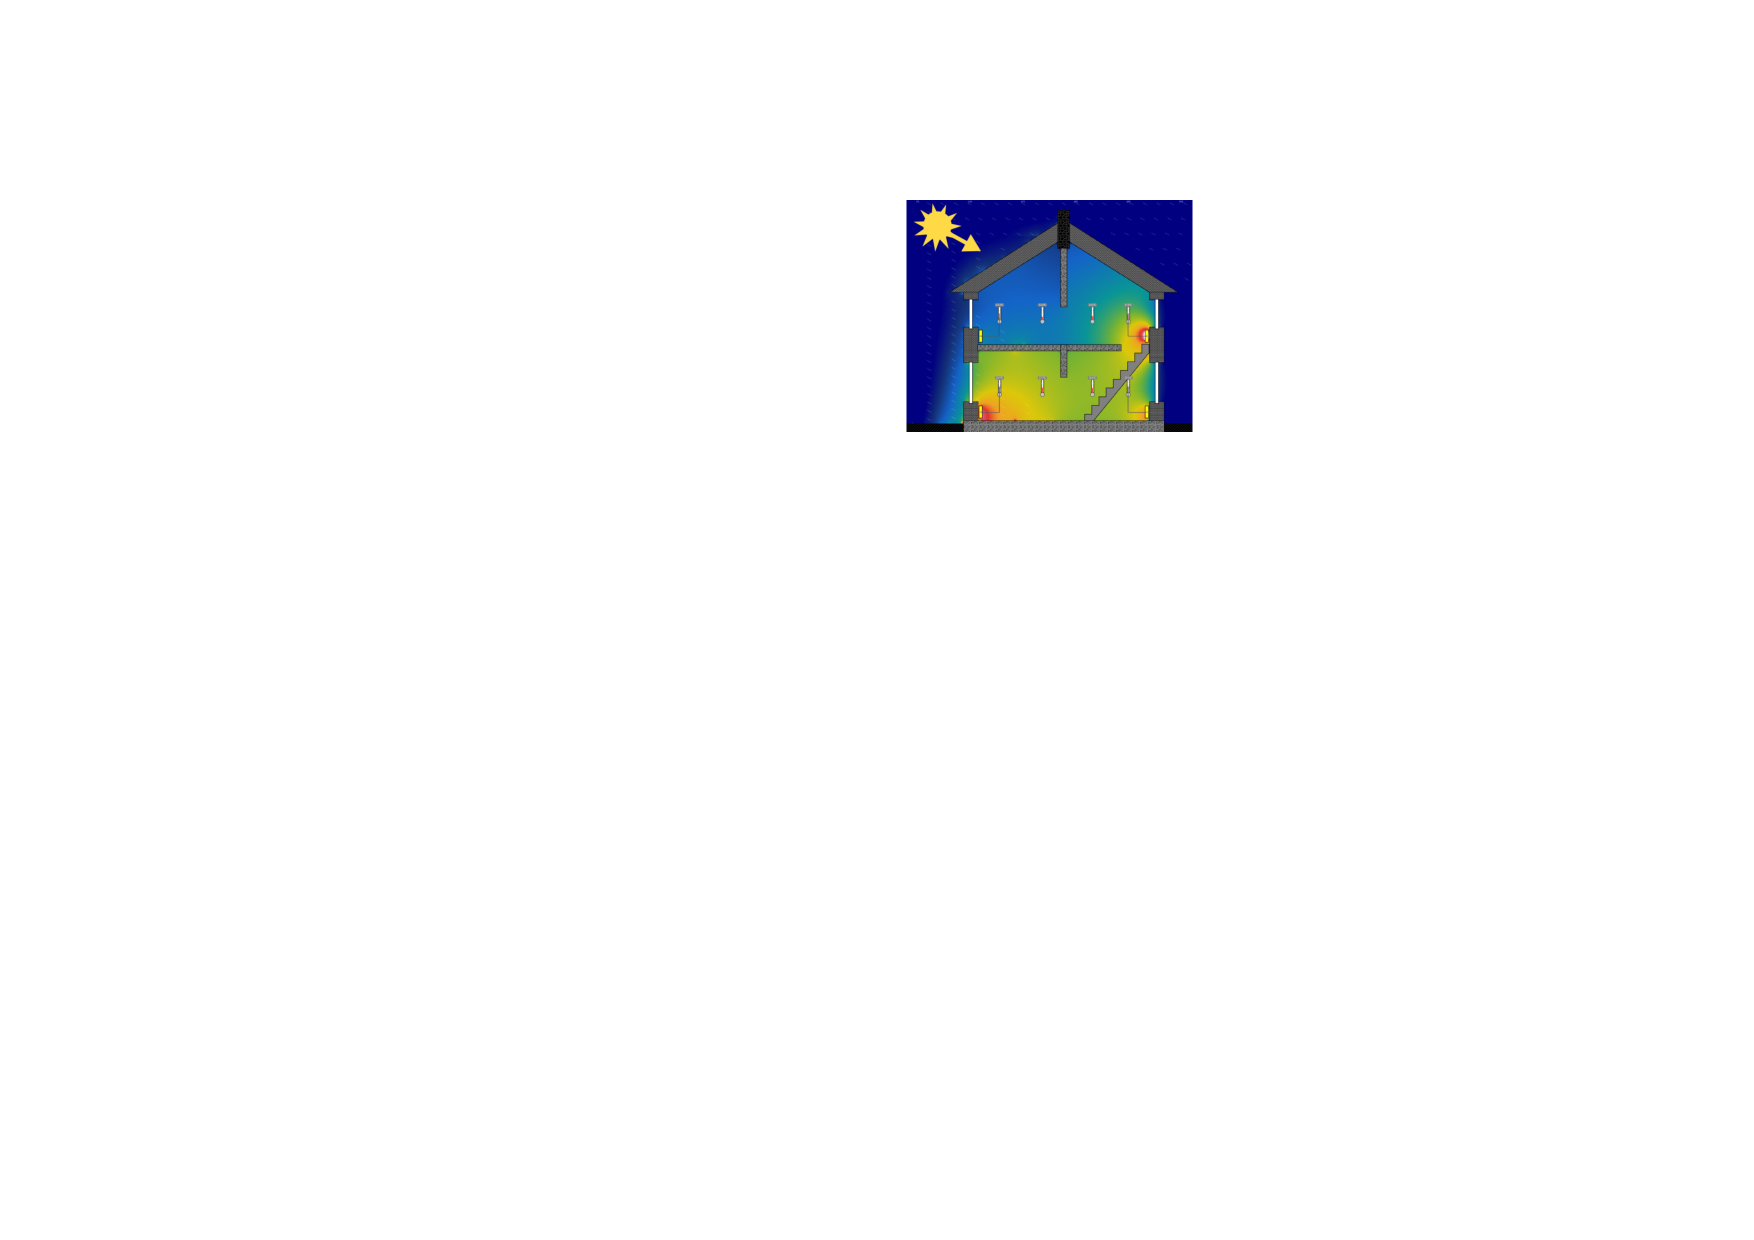
\includegraphics[width=\textwidth]{house-heating/first_iter.pdf}
			\caption{Best setup from BOPP initialization}
		\end{subfigure} \\
		\vspace{10pt}
			\begin{subfigure}[t]{0.47\textwidth}
				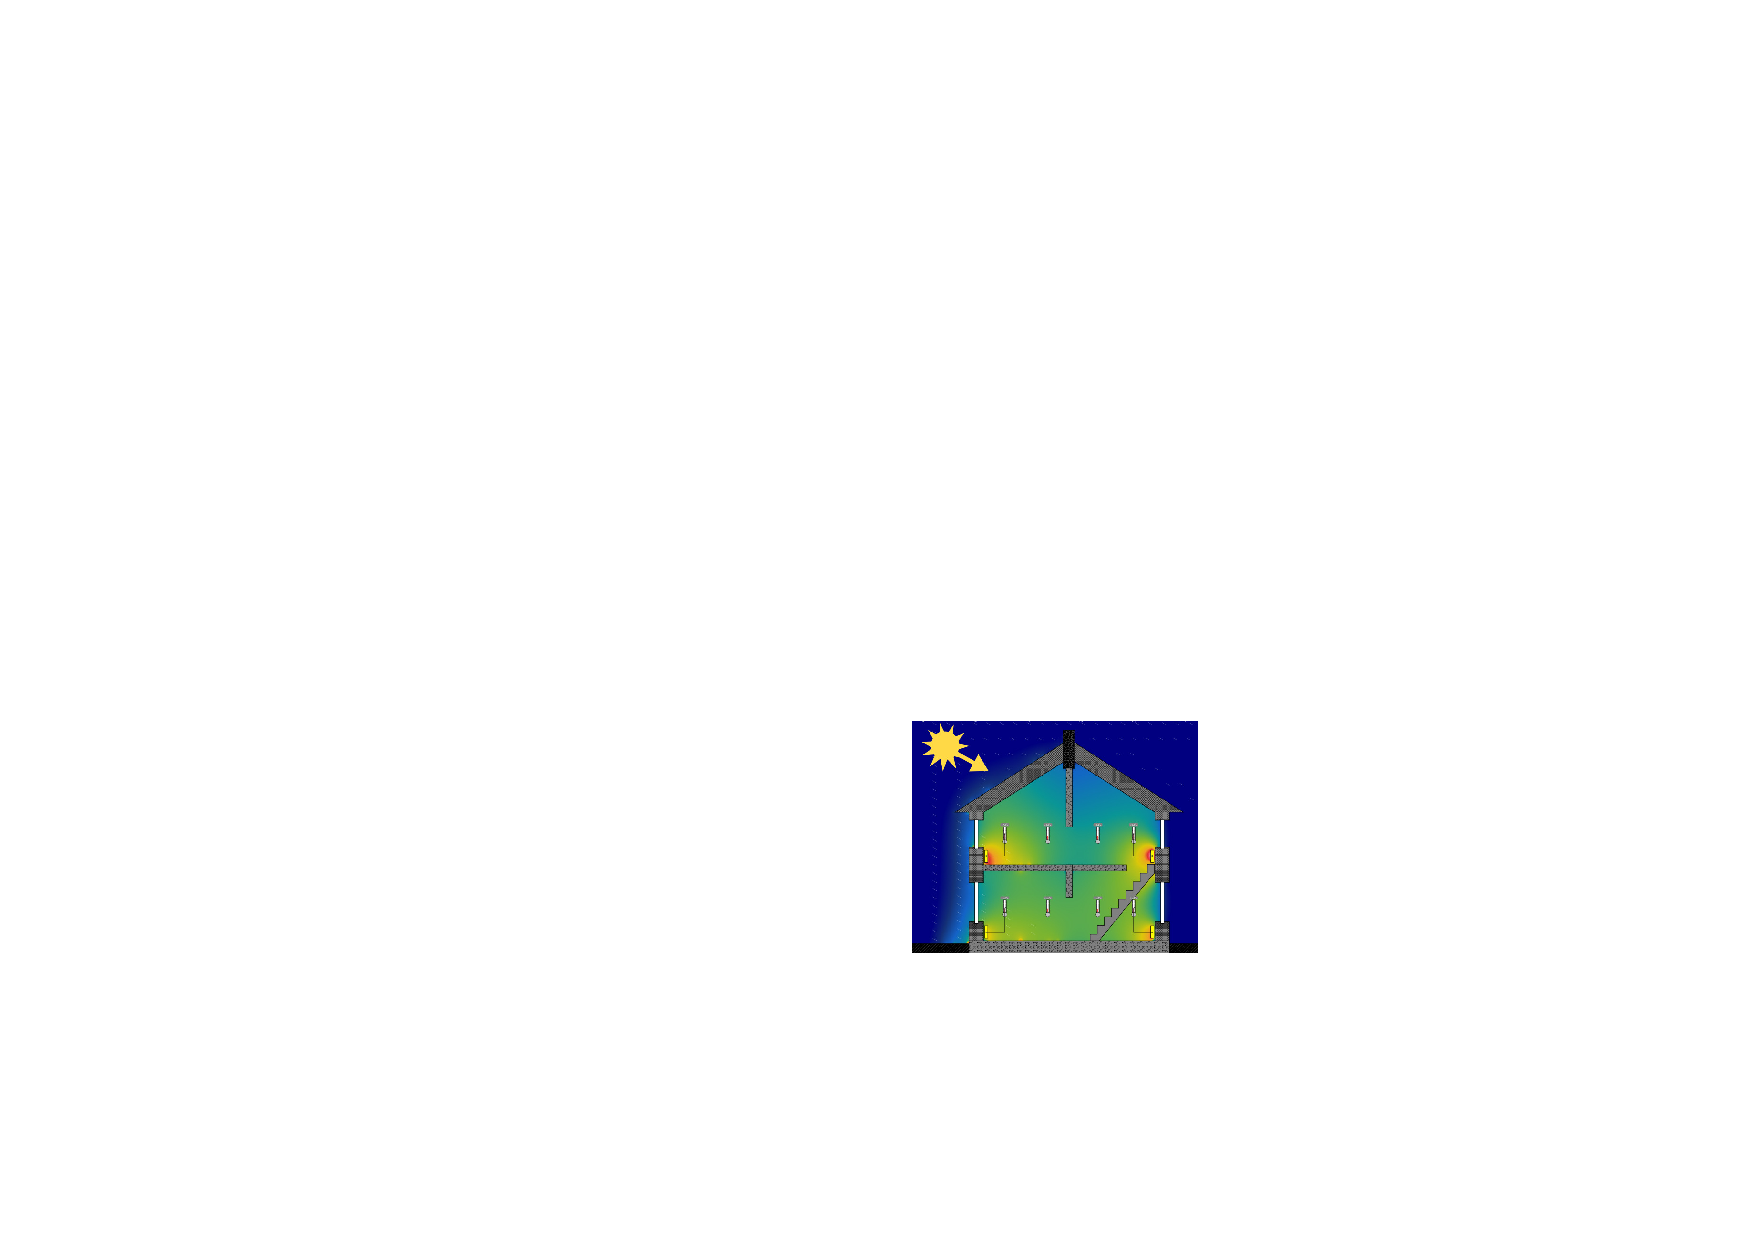
\includegraphics[width=\textwidth]{house-heating/100_iters.pdf}
				\caption{Best setup after 100 iterations of BOPP}
			\end{subfigure}
		~~~~ %	\hspace{40pt}
			\begin{subfigure}[t]{0.47\textwidth}
				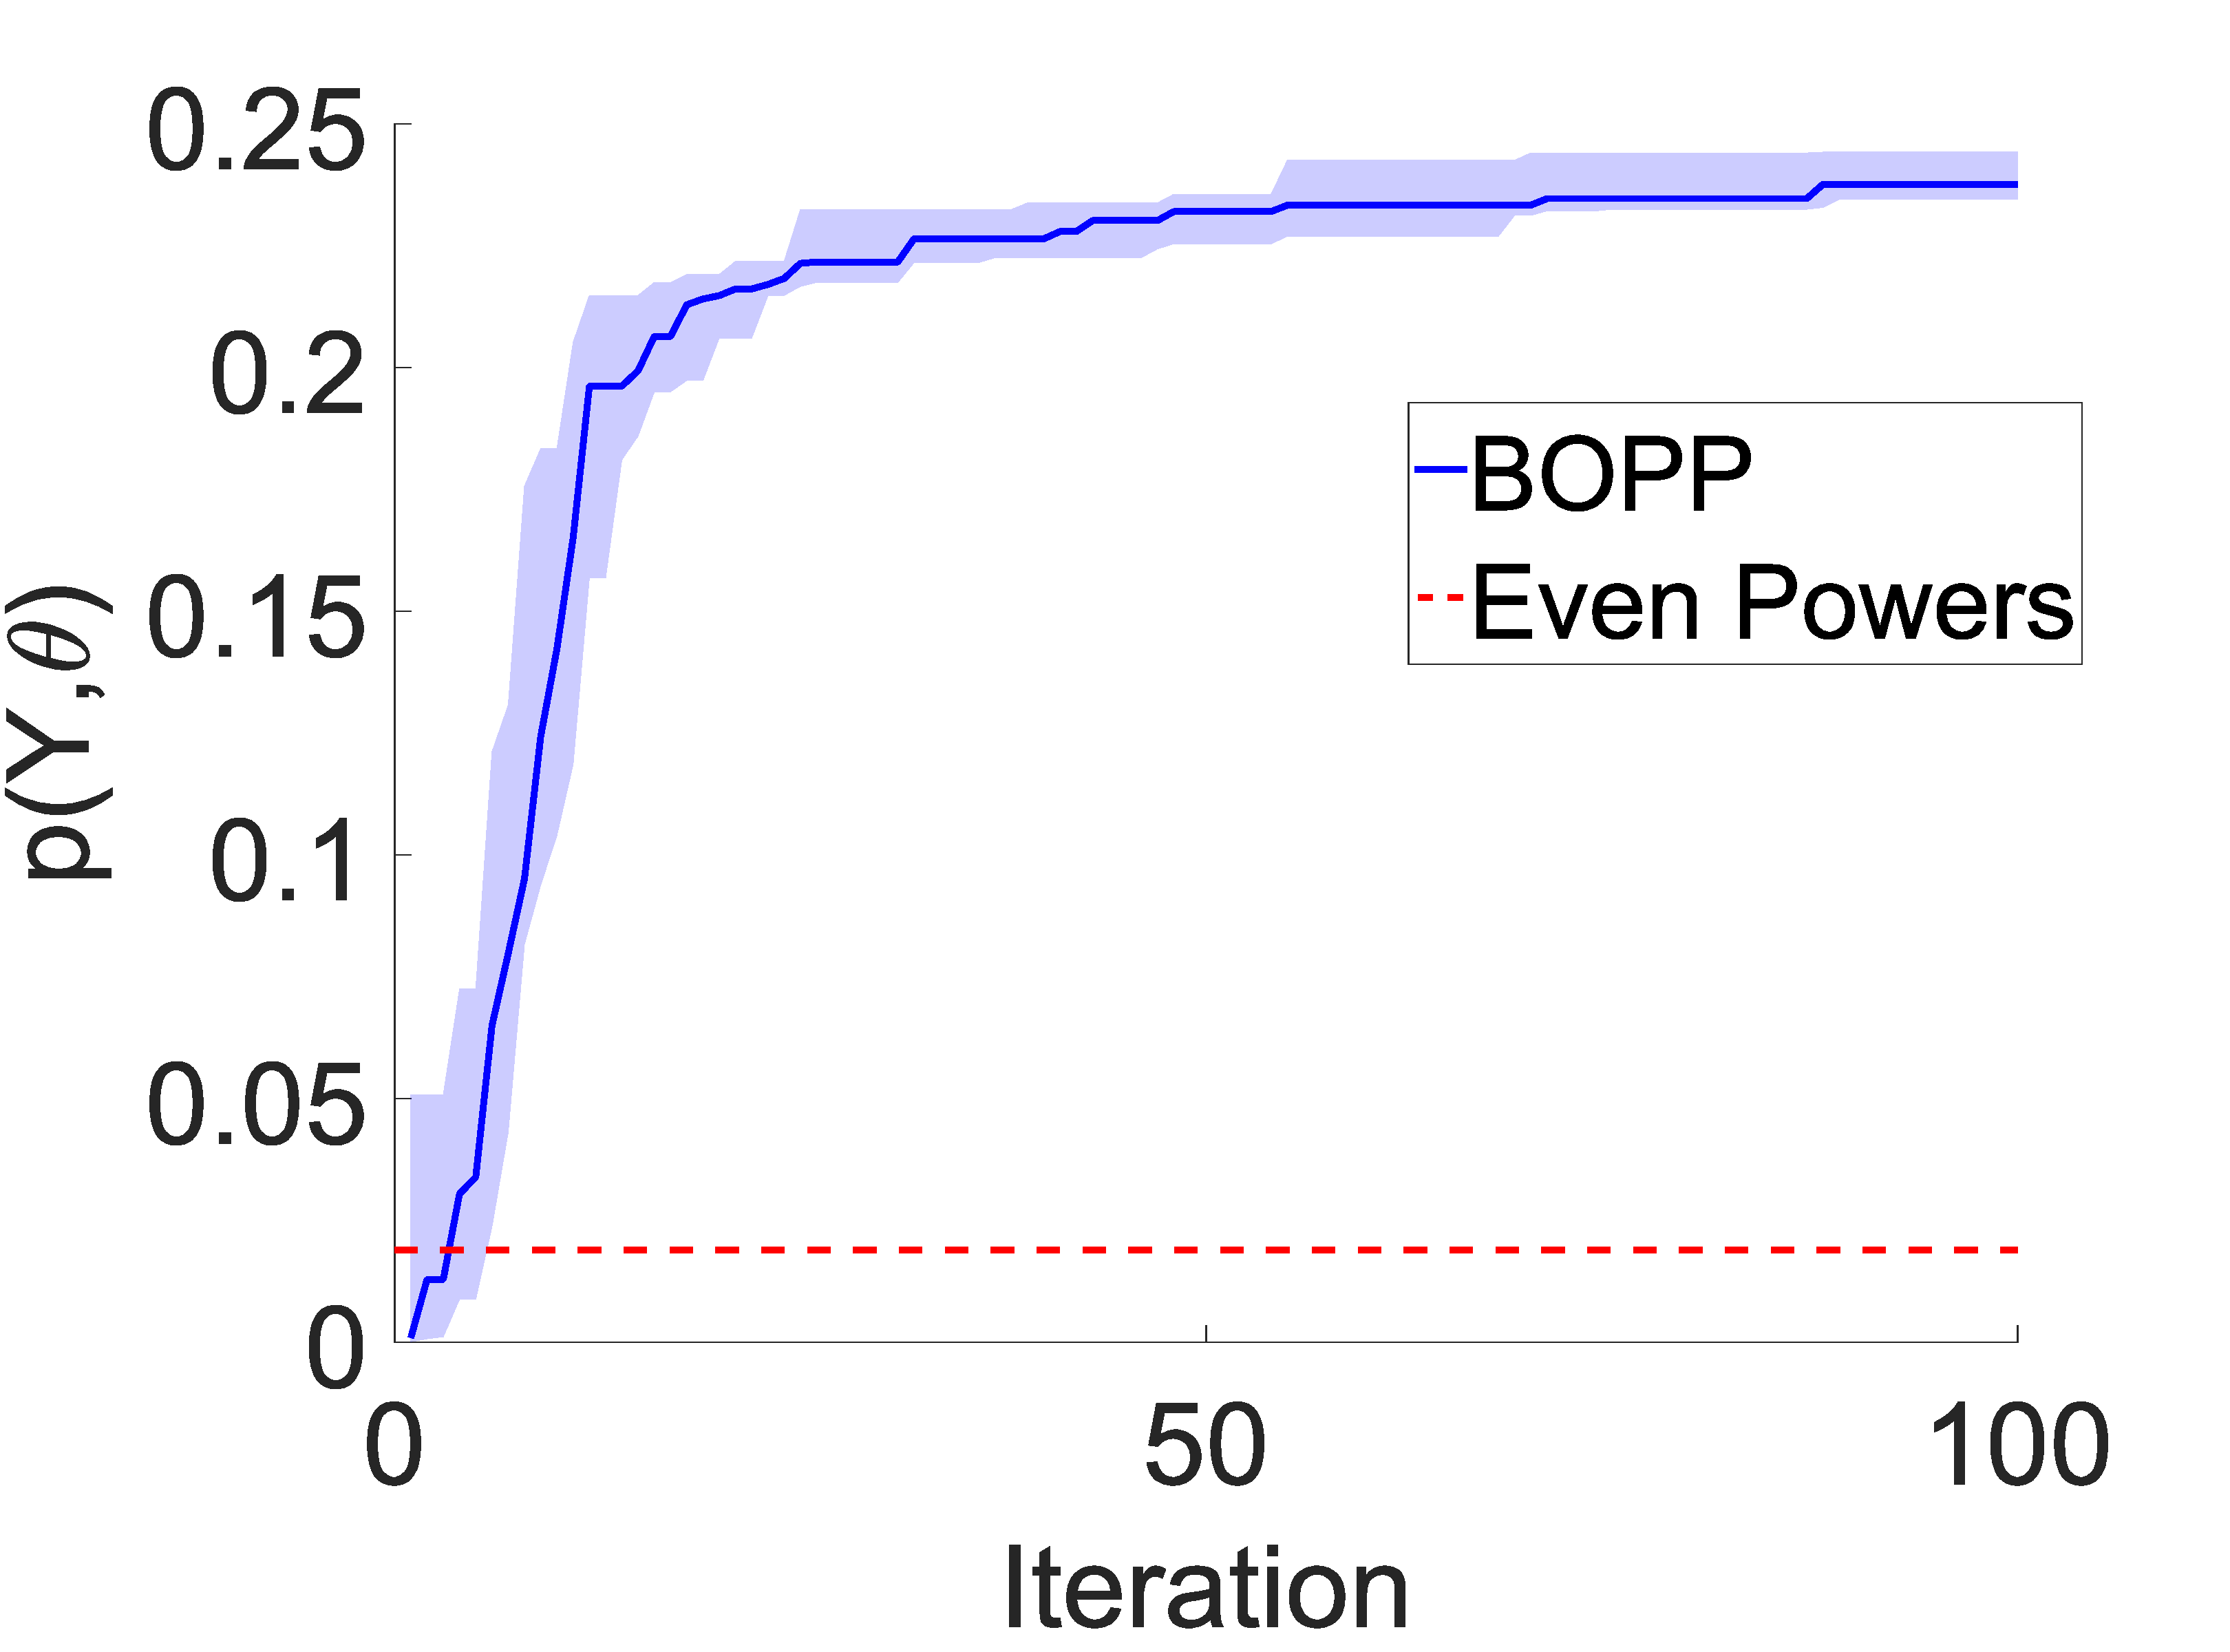
\includegraphics[width=\textwidth]{house-heating/heating_rerun.pdf}
				\caption{Convergence of evidence}
			\end{subfigure}
	% \centering ~~~
	% \includegraphics[width=0.24\textwidth]{"figures/house-heating/probabilistic/logZ-with-even-redblue-wide"}
	%			\caption{
	%				\label{fig:houses-convergence}
	%				Log marginal likelihood $\log Z$ for the \lsi{house-heating} query in Figure~\ref{fig:house-heating-code}. 
	%			}
	%	
	\caption{
		\label{fig:houses}
		Simulation-based optimization of radiator powers subject to varying solar intensity. Shown are output heat maps from Energy2D \citep{xie2012energy2d} simulations at one intensity, corresponding to setting all the radiators to the same power (\emph{top left}), the best result from a set of 5 randomly chosen powers used for initializing BOPP (\emph{top right}), and the best setup found after 100 iterations of BOPP (\emph{bottom left}). The bottom right plot shows convergence of the evidence of the respective model, giving the median and 25/75\% quartiles.
		%Simulation-based optimization of the radiator power subject to varying solar intensity. Here (a-c) show output heat maps from Energy2D \citep{xie2012energy2d} simulations, corresponding respectively to setting all the radiators to the same power, the best result from a set of randomly chosen initializations and the best setup found after 100 iterations of BOPP. (d) shows convergence of the evidence of the respective model as a function of simulation evaluations for independent restarts.
		%Homogenizing the temperature of a 2D model of a house using BOPP. The house has four adaptively controlled radiators, with additional uneven eating is provided by the sun, which will vary both temporally and probabilistically.  Our aim is to select the base power for each of the radiators, subject to some total energy budget, whilst marginalizing out the different anticipated weather conditions.  To do this, the BOPP query given in Figure \ref{fig:house-heating-code} wraps around the finite element heat transfer simulation engine Energy2D \citep{xie2012energy2d} and performs the required MMAP estimation. The na\"ive strategy of setting the power densities of the radiators uniformly (\emph{far left}) leads to an uneven heating\protect\footnotemark, noting that the colormap on the top indicates temperature of air from $5^{\circ}\mathrm C$ to $35^{\circ}\mathrm C$.  
		%After a single iteration of BOPP (\emph{middle left}), the found solution is also poor, but after 100 iterations (\emph{middle right}), a significantly improved solution has been achieved.  The log marginal likelihood in terms of iterations of number of heating setups tested is shown (\emph{far right}) for five separate BOPP runs, along with the resulting marginal likelihood from na\"ively setting the radiators to the same power.
		%Imagine that we have a number of rooms each containing a heating element and we wish to optimize the relative powers of the heaters to deliver the most uniform heating of the house over its lifetime given some total energy budget.  
		% For example, the sun will apply uneven heating to house in a manner which various over time, e.g. due to weather changes and variations in the arc of the sun through the year.  BOPP provides a basis to naturally incorporate these uncertainties into the model, whilst still exploiting the original finite element simulation and returning a single solution the engineer can the go implement.  We therefore believe that in the long term, PPS supporting MMAP have the potential to revolutionise the manner in which engineering simulation is approached by incorporating uncertainty from all stages of the process into a single unified framework, reducing the reliance on fudge-factors and educated guesswork.
	}
\end{figure*}

\begin{figure}[tb]
	\begin{lstlisting}[basicstyle=\ttfamily\small]
(defopt house-heating [alphas target-temperatures] [powers]
 (let [solar-intensity (sample weather-prior)
       powers (sample (dirichlet alphas))
       temperatures (simulate solar-intensity powers)]
  (observe (abc-likelihood temperatures) target-temperatures)))
	\end{lstlisting}	
	\vspace{-6pt}
	\caption{BOPP query for optimizing the power allocation to radiators in a house.  Here \lstinline{weather-prior} is a distribution over the solar intensity and a uniform Dirichlet prior with concentration \lsi{alpha} is placed over the powers. Calling \simulatec performs an Energy2D simulation of house temperatures. The utility of the resulting output is incorporated using \abcl, which measures a discrepency from the \texttt{target-temperatures}. Calling \doopt on this query invokes the BOPP algorithm to perform MMAP estimation, where the second input \lstinline{powers} indicates the variable to be optimized. \label{fig:house-heating-code}}
\end{figure}

Figure~\ref{fig:houses} illustrates how BOPP can be applied to engineering design, taking the example of optimizing the distribution of power between radiators in a house so as to homogenize the temperature, while marginalizing out possible weather conditions and subject to a total energy budget. The probabilistic program shown in Figure~\ref{fig:house-heating-code} allows us to define a prior over the uncertain weather, while conditioning on the output of a deterministic simulator (here Energy2D \citep{xie2012energy2d}-a finite element package for heat transfer) using an ABC likelihood.  BOPP now allows the required coincident inference and optimization to be carried out automatically, directly returning increasingly optimal configurations. 

BO is an attractive choice for the required optimization in MMAP as it is typically efficient in the number of target evaluations, operates on non-differentiable targets, and incorporates noise in the target function evaluations.  However, applying BO to probabilistic programs presents challenges, such as the need to give robust performance on a wide range of problems with varying scaling and potentially unbounded support.  Furthermore, the target program may contain unknown constraints, implicitly defined by the generative model, and variables whose type is unknown (i.e. they may be continuous or discrete).

On the other hand, the availability of the target source code in a PPS presents opportunities to overcome these issues and go beyond what can be done with existing BO packages.  BOPP exploits the source code in a number of ways, such as optimizing the acquisition function using the original generative model to ensure the solution satisfies the implicit constaints, performing adaptive domain scaling to ensure that GP kernel hyperparameters can be set according to problem-independent hyperpriors, and defining an adaptive non-stationary mean function to support unbounded BO. 

Together, these innovations mean that BOPP can be run in a manner that is fully black-box from the user's perspective, requiring only the identification of the target variables relative to current syntax for operating on arbitrary programs. We further show that BOPP is competitive with existing BO engines for direct optimization on common benchmarks problems that do not require marginalization.

%that can be implemented in any PPS where inference methods return marginal likelihood estimates. 



%MMAP estimation is generally difficult as it corresponds to the optimization of an intractable integral, such that function evaluations are expensive and give noisy results.  Current PPS inference engines are typically unsuited to such optimization.  We therefore introduce BOPP (Bayesian optimization for probabilistic programs) which couples existing inference algorithms with a new Gaussian process (GP) \citep{rasmussen2006gaussian} based Bayesian optimization (BO) \citep{osborne2009gaussian, jones1998efficient} package integrated into the PPS Anglican \citep{wood2014new}.  



%MMAP estimation for PPS presents further issues such as the need to be general purpose and robust, whilst dealing with potentially unknown constraints defined implicitly within the generative model.  


%On the other hand, the availability of the target source code in PPS presents opportunities to overcome these issues and go beyond what can be done with existing BO packages.  For example, it allows operation under unknown \emph{equality} constraints and applies automatic domain scaling for problem-independent GP hyperpriors.  In addition to delivering improved performance over prominent BO packages when used simply as an optimizer, these innovations mean that BOPP can be run in a manner that is fully black-box from the user's perspective, requiring only the identification of the target variables relative to current syntax for operating on arbitrary programs.

%\footnotetext{Though results are from the full BOPP implementation with sun heating marginalized out, the simulation plots correspond to a single common condition for the sun for visualization purposes.}

%\section{Motivating Example}
%\label{sec:motivation}


%The rest of this paper is outlined as follows: we first provide background on PPS, BO and GPs.  We define a framework for an optimization query and introduce our core code transformation to allow an arbitrary program to be optimized with respect to parameters defined within the program.  Our algorithm for optimizing the evidence of this program using BO and additional code transformations is outlined, we present experiments demonstrating the applicability of our method and we finish with concluding discussions and suggestions for future work.


\section{Background}

% !TEX root = ../main.tex

\chapter{Probabilistic Programming -- the User's Perspective}
\label{chp:probprog}

Probabilistic programming systems (PPSs) allow users to define probabilistic models 
using a domain-specific programming language or modeling library. A probabilistic program implicitly 
defines a distribution on random variables, whilst the system back-end implements 
general-purpose inference methods.  Two key challenges for a PPS are in providing the
syntax and semantics to allow easy definition of models, and in designing the solvers, i.e.
inference engines, to provide effective inference for those models.
In this chapter, we focus on the former of these, providing an introduction to 
probabilistic programming from a user's perspective, explaining how it can be used for, and
to extend, conventional Bayesian modeling and how it can also be used to reinterpret many computational simulation
techniques not usually associated with Bayesian modeling in a more Bayesian mindset.
We will mostly ignore the rather major issue of how to construct automated inference engines for probabilistic
programs, returning to address this in Chapter~\ref{chp:proginf}.
Here we will explain how general purpose PPSs aim to  provide 
the \emph{flexibility} to define
wide ranging and potentially obscure models, the \emph{expressivity} of a framework for 
model definition that is more in line we conventional scientific simulation than mainstream 
statistical approaches, and the \emph{automation} to  run any problem the user might write
by decoupling model specification and inference.
Together these characteristics produce a framework that allows researchers whose expertise 
lies elsewhere, to carry out powerful statistical analyses for their application specific tasks.  
This framework also aids in the development of both inference
algorithms and models for those within the machine learning and statistics communities,
by removing many of the complications of one while developing the other.
%
%We will for now focus on a user's perspective, introducing how and why one might want to use
%probabilistic programming, explain how ideas from more mainstream Bayesian
%modeling can be transferred, and demonstrate how probabilistic programming can be
%used to both extend the traditional Bayesian framework and reinterpret many computational simulation
%techniques not usually associated with Bayesian modeling in a more Bayesian mindset.
%We will mostly ignore the rather major issue of how to conduct Bayesian inference for
%models defined in probabilistic programs, assuming for now that we have a magical
%general purpose inference engine that will solve any model we provide,
%before returning to actually confront this major stumbling
%block in Chapter~\ref{chp:proginf} once we have introduced the problems of Bayesian
%inference more generally.  We will provide a brief introduction to the Anglican PPS
%to give us a platform for providing examples and highlighting
%key components of designing a PPS.  Finally, we discuss some of the current limitations
%and opportunities for PPSs (other than the obvious computational
%issues which we return to later), in particular demonstrating how we can use them to go beyond
%standard inference frameworks and why we would want to do so.

We note that it will be necessary at times during this chapter to refer briefly to some Bayesian inference
algorithms that will not be properly introduced until Chapters\ref{chp:inf} and~\ref{chp:part}.  
We have situated this chapter before those partly in order to emphasize the point that one should not 
need an intricate knowledge of inference methods to \emph{use} PPSs.  Though it is difficult
to introduce PPSs while completely omitting reference to inference methods, readers who
are not familiar with inference methods should be able to safely ignore which methods are referred to
at a first pass, noting only that different inference algorithms have different requirements and sets 
of problems they perform well on, and thus that the design of a PPS is intricately linked to the inference
method(s) used.

% !TEX root = ../main.tex

\section{Inverting Simulators}
\label{sec:probprog:inv}

Though the use of Bayesian modeling through the sciences and engineering is widespread,
it is still dwarfed by the use of simulators more generally.  Some simulations are inherently
probabilistic, such as many of those used in statistical physics~\citep{landau2014guide},
 financial modeling~\citep{jackel2002monte}, and weather prediction~\citep{evensen1994sequential}.  
 Others are deterministic approximations
of a truly stochastic world, such as lap time simulation for formula one cars~\citep{perantoni2014optimal}
and finite element simulations for fluid dynamics~\citep{versteeg2007introduction}.
In many of these scenarios, real data is also available, but not in sufficient quantities that the carefully
constructed simulations can be done away with entirely and replaced by a purely data driven
approach.  
Imagine the potential utility of general purpose methods for incorporating real data
into these simulators to improve them, without having to throw away the existing carefully constructed models.  
What about if we could even find methods for automatically
inverting these simulators?  Given a target lap time, we could return the best car setup; given observations
of, and a simulator for, human behavior, we could learn about the underlying cognitive processes; given
a climate change model and measurements, we might infer what the driving factors are.  

An ambitious long
term aim of probabilistic programming is to solve such problems and to do so in an automated fashion
so that it requires little or no statistical expertise on the behalf of the user, allowing for simple, widespread usage
across many fields.  The key realization is that stochastic simulators implicitly define probability distributions.
They, therefore, represent generative models and using probabilistic programming we can reason about, and
work with, these generative models explicitly.  One typically thinks of Bayesian modeling in terms of the
prior and the posterior, but one can also think about it in terms of defining a joint distribution over
both parameters and data, then fixing the latter to the actual observations to get a conditional distribution from
this joint.  Simulators implicitly define such joint distributions, with the outputs of the simulator corresponding
to the data, and the inputs and internal variables the parameters.  Probabilistic programming allows us to turn this on its head,
using the same code as the original simulator, but instead providing the observed data as the input and
then inverting the simulator through inference to learn about possible input parameters and other 
variables sampled during the program's forward execution.  
As well as the clear direct utility of allowing such inversion, this process also allows us to improve
our simulator using real data, by calculating the posterior predictive distribution that incorporates both
the original model and the information from the data.

To explain what we mean by inverting simulators more precisely, we will now consider
the example of inferring Captchas~\citep{mansinghka2013approximate}.   Even if the name is not familiar, 
everyone should hopefully have come across Captchas before when a website shows us an image, such
as those in in Figure~\ref{fig:probprog:example_captchas}, and asks us to
type the characters in that image to demonstrate we are not a robot.  We now ask the
question: how might we write an algorithm that breaks this Captcha by 
automatically predicting these characters directly from the image? In other words, 
can we build a robot that mimics a human on a task specifically designed to 
distinguish between the two.  If we had access to large supply of training examples, i.e.
character-image pairs, we could of course use an off-the-shelf discriminative algorithm:
neural networks have been used to try and solve the problem in exactly this way with reasonable
success~\citep{von2008recaptcha}.  However, without access to an abundance of data this is a rather
challenging task and we will need to exploit our prior knowledge about the problem.  

\begin{figure}[t]
	\centering 
	\begin{subfigure}[t]{0.58\textwidth}
		\centering
			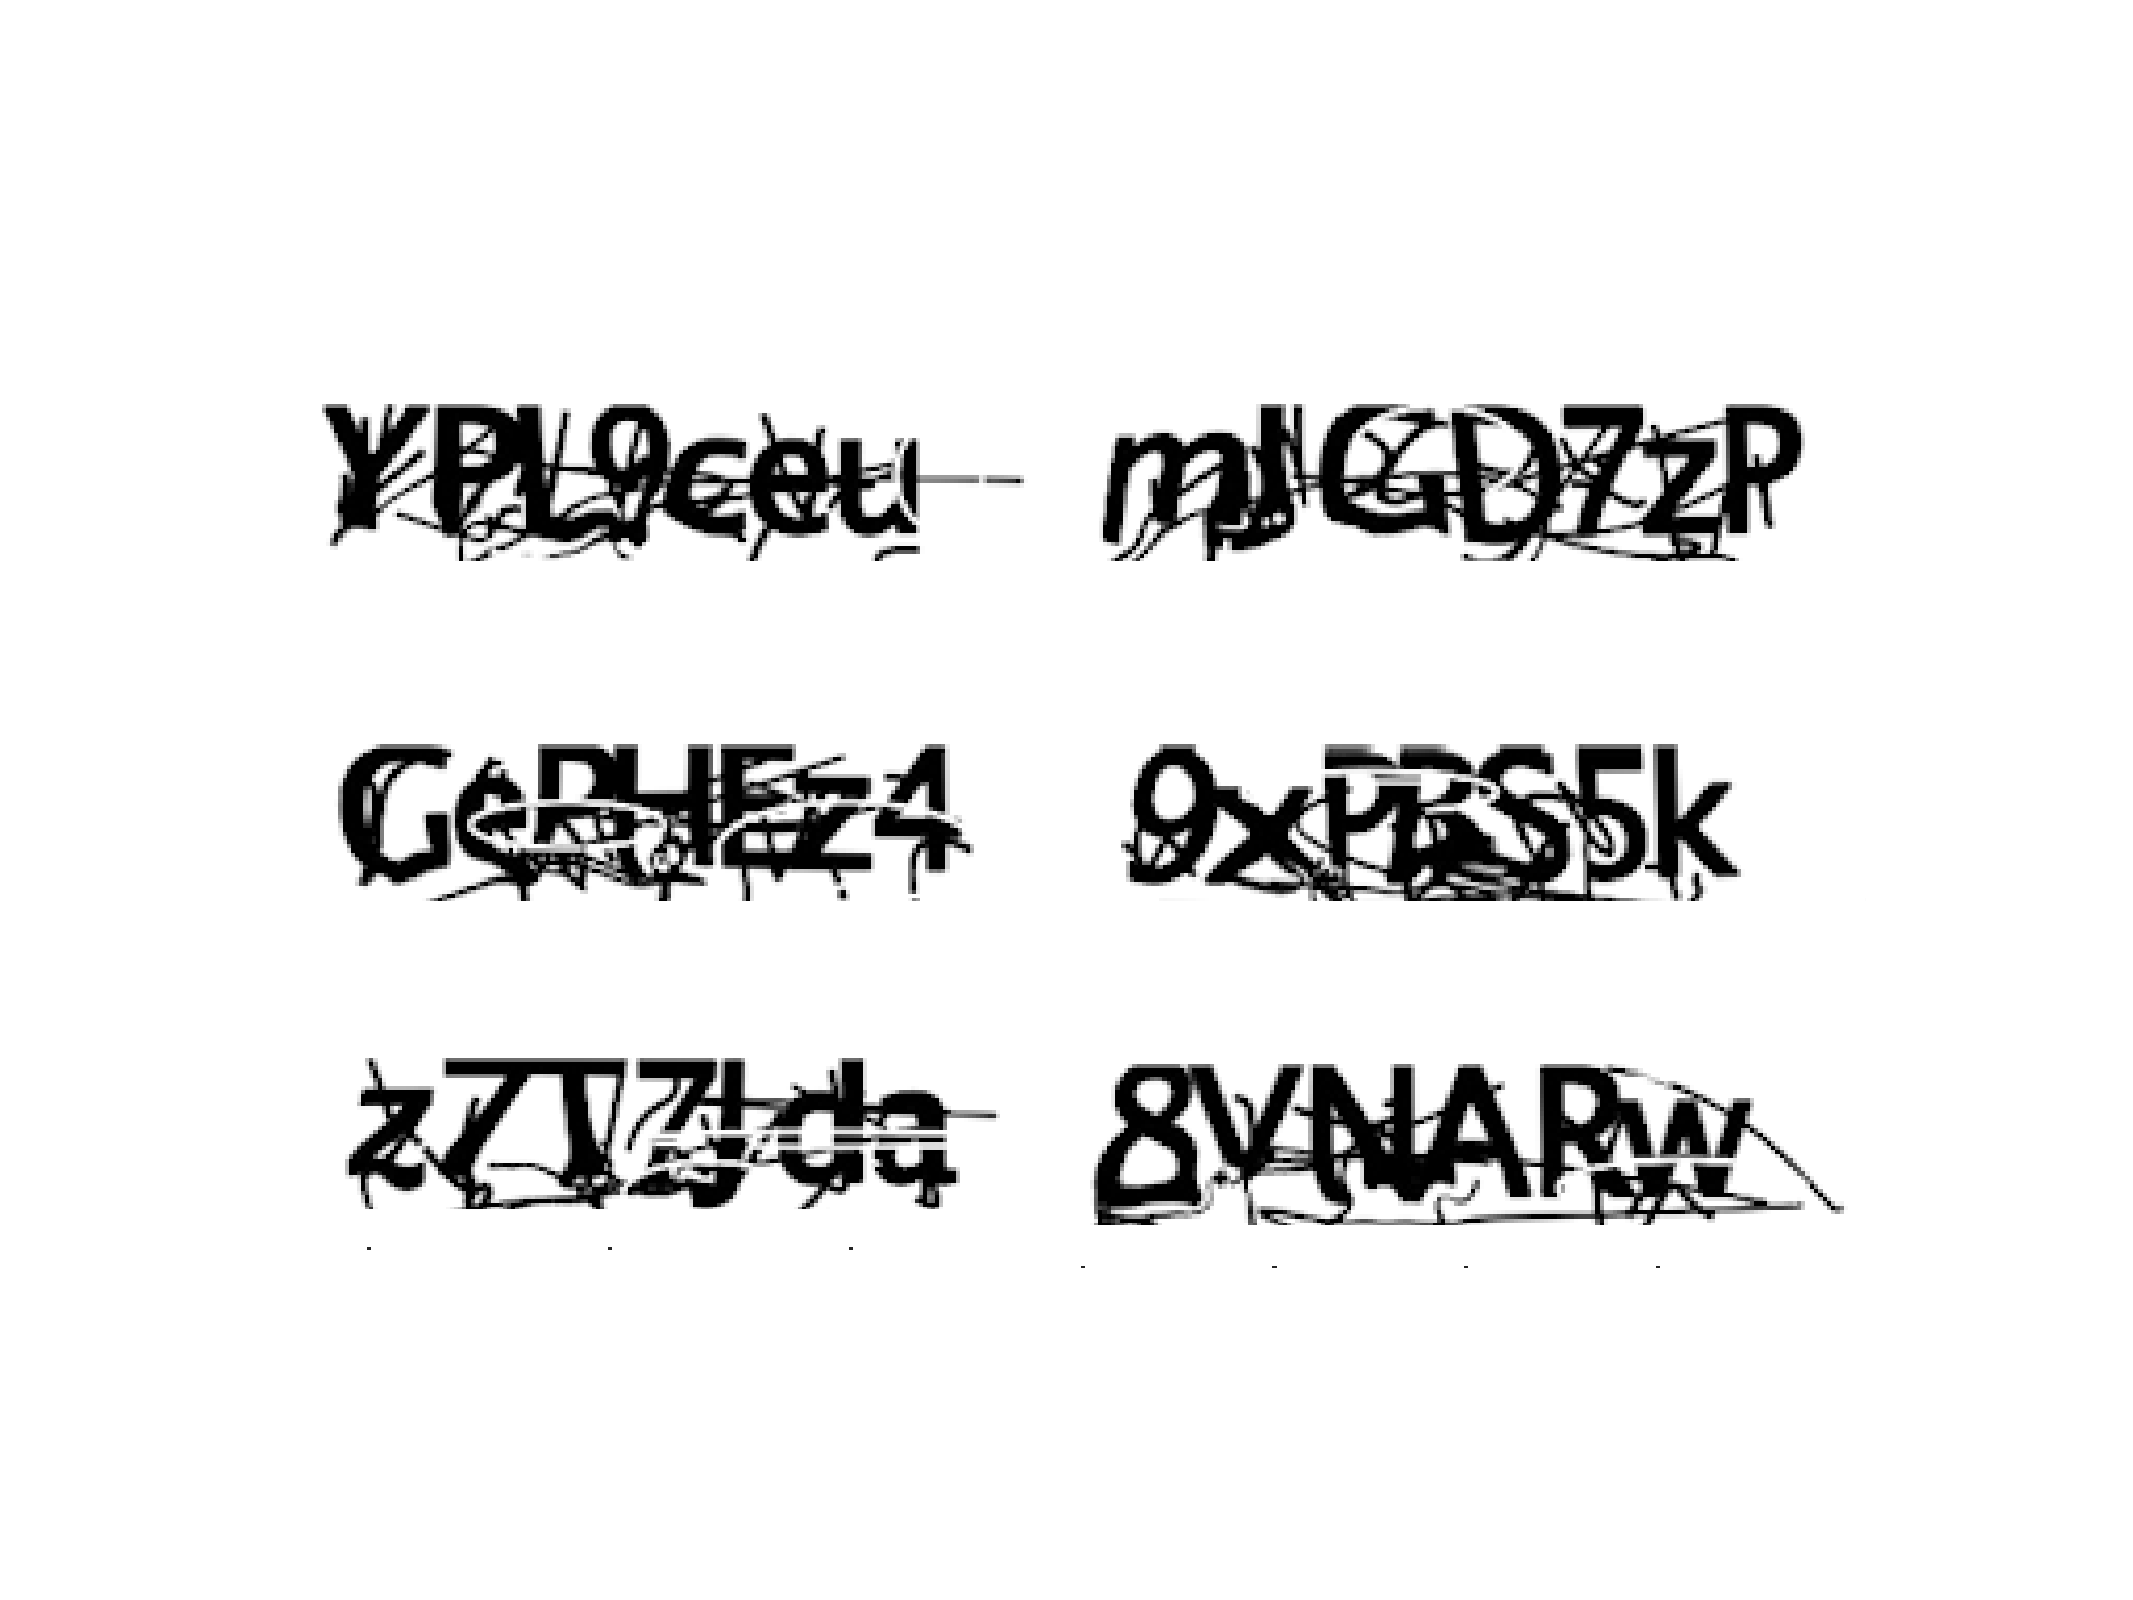
\includegraphics[width=\textwidth]{probprog/figures/example_captchas.pdf}
		\caption{Examples of real Captchas
			 \label{fig:probprog:example_captchas}}
	\end{subfigure}
	~~
	\begin{subfigure}[t]{0.38\textwidth}
		\centering
			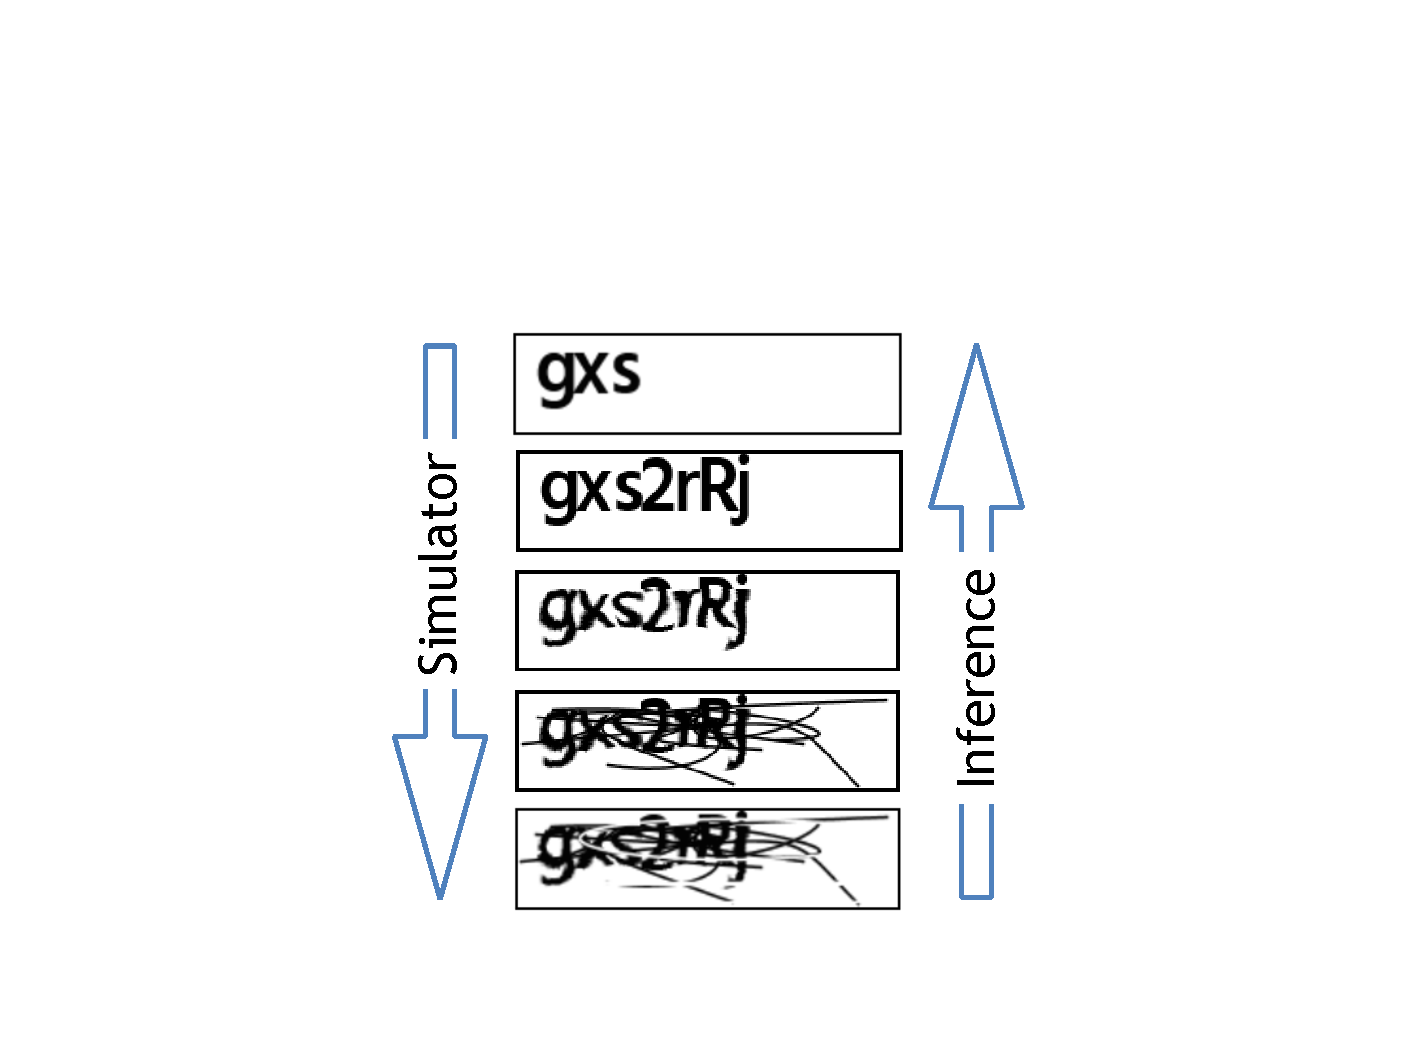
\includegraphics[width=\textwidth]{probprog/figures/captcha_sim.pdf}
		\caption{Example simulation of a Captcha
			\label{fig:probprog:captcha_sim}}
	\end{subfigure}
	\vspace{5pt}
	\caption{Solving Captchas by simulator inversion.   \textbf{(a)} gives examples of real
		Facebook Captchas taken from~\cite{le2017using}.  Here the corresponding
		generating strings going
		to clockwise from the top left are YPL9ceu, mJGD7zP, 9xPBS5k, 8VNARw, z7T7Jda, and
		GePHEz4.  A user is asked to type in these strings when shown the corresponding
		image to show they are not a robot.
		\textbf{(b)} gives an example of the process of simulating Captchas taken by
		~\cite{le2017inference}.  Here we see that we can generate a Captcha by first
		simulating a series of characters, then simulating appropriate manipulations 
		to those characters such as warping, rotating, and adding noise.  Inverting this
		simulation process corresponds to an inference problem, where we want to find
		out the characters that lead to a particular image.
		\label{fig:probprog:captcha}}
\end{figure}

Doing this process in reverse, i.e. simulating a Captcha, on the other hand, is a substantially
less daunting process.  The true Captchas are actually generated by
a simulator and so we can attempt to mimic this original simulation process.
For example, as shown in Figure~\ref{fig:probprog:captcha_sim} we might first sample a 
number of characters, then a symbol for each character, apply manipulations such as rotations and warpings, simulate
some obscuring lines or other noise, and finally render our simulated components into an
image.  Though admittedly it might take some time and effort to construct a high fidelity
simulator that well matches the produced images, the technical requirements for doing this
(other than possibly the final rendering) are minimal and so it could be carried out by most
people with a reasonable degree of experience in scientific programming.  The number of
people able to write such a simulator should certainly be substantially larger than the
number of people with sufficient experience in Bayesian modeling to construct an equivalent
graphical model or direct mathematical formulation.  The number of people
with the expertise to then write an appropriate inference scheme for the problem is even
smaller.  In a PPS, writing this simulator and providing the data is all that is required.
Given these, the PPS will carry out the inference required to invert the simulator automatically,
inferring the characters from the image.  More generally, we are estimating the inputs and
internal variables of our simulator, given target values for the outputs.

There are two key factors to realizing our aim of inverting simulators.  Firstly we need to provide a 
language which easily allows users to
write down simulators and which has semantics that allows the compiler to extract an appropriate
representation of the joint distribution.  In other words, we need our language to be sufficiently
general purpose and easy to use to not burden the user, while at the same time having syntax and semantics that
ensure the corresponding joint distribution is well defined and can be converted into a form where
we can run inference.  Doing this will require the introduction of means for \emph{conditioning} on data
and of specially defined \emph{random primitives} whose behavior can be controlled at 
run time, rather than just always sampling from
the same predefined distribution as they would in an ordinary programming language.  
The latter can be thought of as defining terms in the prior and the
former as terms in the likelihood as we will discuss in Section~\ref{sec:probprog:models}.
For certain cases, one can alternatively think of conditioning as applying \emph{constraints} to the
program.  For example, we can think of a probabilistic program as defining a simulator
and a set constraints that must be satisfied; this is exactly
how the PPS Church~\citep{goodman2008church} is designed.  An important distinction 
here though is between \emph{hard} and \emph{soft} conditioning.  Hard conditioning is as per the conventional
interpretation of a constraint -- we condition on the fact that an event occurs exactly.  Soft conditioning instead
assigns a weight to the program based on the probability (or probability density) of a given event occurring.
Though hard conditioning is a particular case of soft conditioning (for which the weight is either 1 or 0),
one can, at least semantically, use it to specify a soft conditioning, say 
$p(Y=y | X=x)$, by sampling $Y\sim p(y|X=x)$ and then imposing the constraint $Y=y$.
However, only supporting hard conditioning in a PPS is somewhat restrictive for practical
use, as one cannot effectively condition on continuous data because there is zero probability of
satisfying the resulting constraint.

The second key factor is that our language needs a general purpose inference(s)
engine capable of working on any program the user writes.  Bayesian models are fully defined
by their joint distribution and the data.  Therefore, once a user has written their simulator and provided
the data, this uniquely defines a posterior and the only problem is in solving the resulting Bayesian inference.
If we can now construct inference engines capable of working on arbitrary code, we can 
automate inference on any simulator or model the user defines, creating an
abstraction barrier between model definition and drawing inferences from that model.  We will discuss how this can be
done at length in Chapter~\ref{chp:proginf}.

If we can construct a system that can successfully carry out these tasks, 
the huge potential applications this could provide should be clear. We would have a 
system where the user requires no expertise in inference or conventional
Bayesian modeling in order to write application specific models and have them solved automatically.
Instead, they need only have the ability to write stochastic simulators for the process they wish to
model, a skill possessed my most of the scientific community and many of those outside it as well.
In a hypothetical future where scientists
code all their simulators in extremely powerful PPSs, tasks such as
inverting those simulators and improving the simulator by incorporating real data would
be automated in the same way current compilers convert high-level coding languages to machine code.  
However, this ability is not completely
hypothetical -- many such problems can already be handled by existing systems.  The challenge
is improving and scaling such systems to deal effectively with more difficult and more wide ranging models
in a tractable manner.  The need for such systems to work in an automated manner for a wide array
of possible problems makes this a very difficult problem; after all we are somewhat flaunting the no-free-lunch
theorem.  However, there is a key component that provides hope that this may be possible: we have access
to the target source code of the simulator itself, rather than needing to treat it as a black-box as is the
case for, say, approximate Bayesian computation (ABC) methods~\citep{csillery2010approximate}.  Therefore
maybe we can have our cake and eat it by using the source code itself to guide our algorithms, such that
they behave in problem specific ways.  We will discuss how this can be done at length in 
Chapters~\ref{chp:proginf} and~\ref{chp:bopp}.
% !TEX root = ../main.tex

\section{Differing Approaches}
\label{sec:probprog:two}

Rather than being a clearly defined method,
probabilistic programming is more of an umbrella term that covers a spectrum of 
different approaches, varying from inference toolboxes through to universal probabilistic programming
languages (PPLs) that allow
arbitrary probabilistic code to be written.
%, even that which might not correspond to a valid model.  
Often there is a trade-off between efficiency and expressivity: the more restricted
one makes the language, the more those restrictions can be exploited to improve the efficiency
of the inference.  This leads itself two distinct philosophies when developing a system. 
Firstly one can start with a particular inference algorithm and then design a system around making it as
easy as possible to write models for which that inference algorithm is suitable.  Secondly one can start
with  a general purpose PPL that allows as many model as possible to be written and then try to construct
inference engines that are capable of work in such a general framework.  Both approaches 
have their merits and drawbacks, with the distinction typically coming down to the intended use.
We will now elucidate each approach more precisely.  

\subsection{Inference Driven Systems}
\label{sec:probprog:two:inf}

Though there is a plethora of bespoke inference algorithms designed for particular models, the vast majority of these are based around
a relatively small number of foundational methods such as importance sampling, sequential Monte Carlo,
Metropolis-Hastings, Gibbs sampling, message passing, and variational inference (see Chapter~\ref{chp:inf}).
The extensive use of these core inference approaches throughout Bayesian statistics and machine
learning means that it makes clear sense to write packages for automating them and which
make it easy for the user to define an appropriate graphical models for which the inference can be automated.
This both improves efficiency of modeling and reduces barriers to effective Bayesian modeling by reducing the
required inference expertise for users.  This inference-first philosophy is taken by a number of successful PPSs
and inference toolboxes (the distinguishing line between which can be a little blurry), a small number of which we now 
briefly outline.

BUGS (Bayesian inference Using Gibbs Sampling) \citep{spiegelhalter1996bugs} and its 
	extensions~\citep{lunn2000winbugs,plummer2003jags,todeschini2014biips}
	allow finite DAGs to be specified using declarative code or pictorially using a graphical user
	interface.  These are converted to a form that is suitable for inference, the exact nature of which
	depends on the implementation, with the original work being based on Gibbs sampling.
	
Infer.Net \citep{minka_software_2010} is modeling language for defining, and automating approximate inference in
	both DAGs and Markov random fields, using predominantly message-passing algorithms. Distributions
	are generally, though not exclusively, restricted to be exponential families.  Branching (i.e. \texttt{if}) 
	is allowed, but requires enumeration of all possible paths at run time.

LibBi \citep{murray2013bayesian} is a package for doing Bayesian inference for state-space models,
	using particle-based inference methods (see Chapter~\ref{chp:part}).  It has a strong focus on scalable
	computation, providing support for multi-core architectures and graphics processing units.

PyMC3 \citep{salvatier2016probabilistic} is a python framework for carrying out MCMC and variational
	inference, using Theano~\citep{bergstra2010theano} to calculate the gradients required by some inference methods.

Stan \citep{carpenter2015stan} is a PPS with interfaces to many difference languages and a
	focus on performing Hamiltonian Monte Carlo inference~\citep{duane1987hybrid,hoffman2014no}, though
	other inference methods such as variational inference are also provided~\citep{kucukelbir2015automatic}.
	As with PyMC3, automatic differentiation is used to calculate required gradients.  The need to take
	derivatives means that there is limited support for discrete variables or branching.

These systems do not allow users to write models that would be difficult (at least for
an expert) to code without a PPS -- in general they all can be thought of as defining a graphical model
or sometimes factor graph -- but they offer substantial utility through ease of model exposition and
automating inference.

\subsection{Universal Probabilistic Programming}
\label{sec:probprog:two:general}

As useful as these inference-driven systems are, they do not fit very well with the notion of
inverting simulators we introduced in Section~\ref{sec:probprog:inv}.  They are still closely tied
to graphical models and are more toolboxes for streamlining the Bayesian modeling process than
a means of writing models that would be problematic to define by conventional means.  Achieving
our long term ambitious aim of making general purpose systems for conducting inference of
arbitrary simulators will require us to take a somewhat different approach that instead starts
with a general-purpose language and then attempts to design inference algorithms capable of
working on arbitrary models and code.  It will be necessary for such systems to
support models where the set of random variables is dynamically typed, such that it is possible 
to write programs in which this set, and thus potentially the number of random variables, differs 
from execution to execution.  To avoid hindering the user or restricting the models which can be
defined, it will important to allow 
things such as branching, recursion, higher-order functions,
conditional existence of variables, and arbitrary black-box
deterministic functions.  Ideally, we would like to provide no restrictions on the code that the user
can write, except for eliminating programs do not define valid probability distributions, such as
those that have a non-zero probability of never terminating.  In practice catching such invalid cases can
be hard or even impossible and so many systems actually adopt a philosophy of applying no restrictions,
such that it is perfectly possible to define invalid models.  General purpose PPSs actually bring up new
theoretical questions about what constitutes a valid probability model~\citep{heunen2017convenient}, while
even the set of valid definable models is a strict super-set of the those definable by graphical models 
for many systems~\citep{goodman2013principles}.

In the rest of this thesis, we will predominantly focus on these \emph{universal} PPLs~\citep{goodman_uai_2008,staton2016semantics}, 
so-called because they are based on \emph{Turing complete} languages that can specify any
computable distribution~\citep{goodman2013principles}.  For our purposes, we further refine this definition
to systems that also allow specification for any computable conditioning.
We will regularly using the universal PPL Anglican~\citep{wood2014new} as a reference, an introduction
to which is provided in Section~\ref{sec:probprog:anglican}. Here we will briefly discuss some other
prominent higher order PPLs.

Church is a PPL based on Scheme \citep{goodman_uai_2008}.  
The original seminal paper and accompanying system 
	forms a foundation on which many of the prominent existing systems are built through its
	demonstration that higher-order probabilistic programs define valid probability models, even in
	the presence of infinite recursion.  However, Church predominantly only allows hard
		conditioning,\footnote{Some very limited support for soft-conditioning is provided in current
		implementations through a ``noisy equals'' that equates to a Gaussian likelihood.}
	namely a model in Church comprises of a generative sampler and a separate predicate procedure
	which returns true if the desired conditions are satisfied.  
	In addition to the aforementioned issues of hard conditioning, this complete separation of the 
	generative process and the conditioning can also be wasteful in not allowing the structure of a 
	model to be exploited (see Chapters~\ref{chp:part} and \ref{chp:proginf}).  
	Later systems therefore mostly allow soft conditioning statements to be interleaved
	through the generative progress (in an analogous manner to likelihood terms), increasing the range
	of (solvable) models than can be encoded and the potential efficiency of inference algorithms.
	Inference in Church (and its direct derivatives) is typically carried out using either rejection sampling
	or MCMC.  Church places a particularly strong emphasis on the ability to carry out \emph{nested inference},
	something we will look into in depth in Chapter~\ref{chp:nest}.

Venture~\citep{mansinghka2014venture} is a probabilistic programming platform providing a flexible
system for both specification of models and inference methods.  In has a strong emphasis on being extensible
and for allowing the hosting of eternal applications.  For example, it allows the user to provide proposals for
the inference engine or reprogram the inference strategy entirely.  Venture is predominantly used via the
VentureScript~\citep{mansinghka2014venture} PPL.

WebPPL \citep{goodman_book_2014} is a PPL built using a purely functional subset of Javascript,
conveniently allowing for embedding in web pages.
In combines the ability to write a generative process using sampling statements and to add in likelihood
terms through a {\small \texttt{factor}} primitive that is analogous to the \observe primitive that we will introduce
in Section~\ref{sec:probprog:models:first}.  At its back end, WebPPL provides a number of different inference
algorithms, such as SMC and MCMC methods.

The price for the expressivity of these general purpose systems is a substantial extra 
burden on the inference engine as we will
discuss in Chapter~\ref{chp:proginf}.  In general, inference methods for such systems 
must be formulated in such a manner that they are applicable to models where the 
density function is intractable and can only be evaluated during forwards simulation of the program. 
For example, it may not be possible to know if a variable is continuous or discrete except by
running the program, while some variables will only exist conditioned on the values of others.
This required generality of the inference engine will naturally lead to a drop in performance compared to
custom written inference code, but this is often a price worth paying for generality and automation, particularly
when considering models that would be challenging to express, let alone do inference in, using more
conventional frameworks.
% !TEX root = ../main.tex

\section{Bayesian Models as Program Code}
\label{sec:probprog:models}

In the last section we shown how we can thing of PPS as inverting simulators, predicting internal
variables and the inputs given the outputs.  In this section we will take a different perspective and
show how we can translate Bayesian modeling into the framework of program code.  As we 
showed in Chapter~\ref{chp:bayes} we showed how a Bayesian model is defined by a prior over
parameters and a likelihood function for those parameters given the data.  This viewpoint will
mostly translate into the probabilistic programming setting by equating between the prior
and sampling statements and between the likelihood and conditioning statements.  At the end
of the section we will explain why this is actually a slight approximation (in short because we
might condition on internally sampled variables) but for most purposes this viewpoint will suffice.
We will keep things predominantly high-level for now, giving a more detailed look in
Section~\ref{sec:probprog:anglican} by introducing a particular PPS, namely Anglican, in detail.

\subsection{A Simplified Probabilistic Programming Setup}
\label{sec:probprog:models:first}

We start by considering the case of constructing a restricted PPS.  We will presume that our
language has no branching (i.e. no \texttt{if} statements or equivalent), is  first order
(i.e. variables cannot be functions), that there is no recursion, and that it does not allow 
any conditioning on internally sampled variables.  
We will give our language
two special constructs, \sample and \observe, between which the distribution of the
program is defined.  As such the program should not include any other random components.
Informally, \sample will be used to specify terms in the prior and \observe terms in the
likelihood.  More precisely, \sample will be used to make random draws $x_t \sim f_t(x_t | \Xi_t)$,
where $\Xi_t$ is a subset the other variables in scope at the point of sampling, and \observe will use to condition on
data $g_s(y_s|\Lambda_s)$ with $\Lambda_s$ defined in the same way as $\Xi_t$.  We presume that the program takes 
in as input external parameters $\theta$ and data $y_{1:S}$, the former of which is taken as inputs that are 
not ``observed'' at any point but can effect the conditioning through $\Xi_t$ and $\Lambda_s$, while we presume 
for our simplified setup that the latter appears in neither $\Xi_t$ or $\Lambda_s$.
We define both \sample and \observe as adding a factor to the joint distribution which is therefore given by
\begin{align}
\label{eq:probprog:simple-joint}
p(x_{1:T},y_{1:S} | \theta) = \prod_{t=1}^{T} f_t(x_t | \Xi_t) \prod_{s=1}^{S} g_s(y_s|\Lambda_s).
\end{align}
The two vary in whether they define a new random variable or effect the probability of the
program given particular instances of the other random variables.
Our presumptions for this simplified setup that no $y_{s}$ terms are present in the $\Xi_t$ or $\Lambda_s$
and that we do not condition on internally sampled variables, means that we can here have
exactly that our prior is $\prod_{t=1}^{T} g_t(x_t | \Xi_t) =: p(x_{1:T} | \theta)$ and our likelihood is
$\prod_{s=1}^{S} g_s(y_s|\Lambda_s) =: p(y_{1:S} | x_{1:T}, \theta)$.  Consequently, for our simplified setup,
each program defines a finite directed acyclic graphical model (see Section~\ref{sec:bayes:paradigm:graph})
where the conditional relationships are defined through the definitions of $f_t$ and $g_s$.
This breakdown into a prior and likelihood and the equivalence to graphical models
will not hold in the more general cases we consider later.  \todo[inline]{Some example programs and equivalent
	graphical models for our simplified setup are given in Figure INSERT}

An important point to note is that~\eqref{eq:probprog:simple-joint} shows that all of our \sample
and \observe statements are exchangeable, in the sense that their order can be moved around and
still define the same joint distribution, up to restrictions about all the required variables required
for the conditioning existing and being in scope.  For example, if all variables remain in scope
and are not redefined, we can generally move all our \observe statements to the end of the program
without changing the joint distribution.  Nonetheless, the position of the \observe statements
can often be important from the perspective of the performance of the inference engine.  This exchangeability
result will carry over to the non-simplified cases.

Other than \sample and \observe statements, the rest of our program is by construction totally deterministic.  Therefore,
though it may contain random variables other than $x_{1:T}$, these random variables are deterministic
functions of the ``raw'' random draws $x_{1:T}$ and inputs $\theta$ and $y_{1:S}$.  We can therefore 
define the outputs of our program as $z := h(x_{1:T},y_{1:S},\theta)$ for some deterministic function $h$.
As we explained in Section~\ref{sec:prob:measure}, the change of variables means that the density function on $z$,
$p(z | y_{1:S}, \theta) $
can have a different form to the posterior implied by our program, namely $p(x_{1:T} | y_{1:S}, \theta)$.
  Though this is a serious complication in the
context of optimization (we may not in general be able to find $\argmax_z p(z|y_{1:S},\theta)$
or even evaluate $p(z | y_{1:S}, \theta)$ exactly), it
is perfectly acceptable in the context of calculating expectations as
\begin{align}
\int f(z) p(z | y_{1:S}, \theta) dz = \int f(h(x_{1:T}, y_{1:S}, \theta)) p(x_{1:T} | y_{1:S}, \theta) dx_{1:T}
\end{align}
for implicitly defined measures $dz$ and $dx_{1:T}$.  Two consequences of this are that
we can express any expectations calculated by our program as expectations over $p(x_{1:T} | y_{1:S}, \theta)$
which was fully defined by the joint~\eqref{eq:probprog:simple-joint} and that, provided we are not worried
about carrying out optimizations, we do not need to explicitly worry about the implicit measures defined
by the definition of our program, other than any potential effects on the inference scheme.


%
%Because of the assumptions we have made for our language, the latent
%variables we wish to do inference for are statically determined as $x_{1:T} = x_1,\dots,x_T$ 
%such that the posterior of interest is $p_{\theta} (x_{1:T} | y_{1:S})$ (or some marginal of this for
%which we can still using Monte Carlo inference on the joint).
%
%Our implied target posterior
%is proportional to this joint in the standard way $p_{\theta}(x_{1:T}|y_{1:S}) \propto p_{\theta}(x_{1:T},y_{1:S})$.

\subsection{A General Probabilistic Programming Setup}
\label{sec:probprog:models:general}

Note that as $y_s$ terms can appear in the $\Xi_t$ terms, it can be the case that 
$p(x_{1:T} | \theta) \neq \prod_{t=1}^{T} p(x_t | \Xi_t)$ such that the latter does not
ex
can also enter \sample or \observe terms through $\Xi_t$ and $\Xi_s$ respectively.

\todo[inline]{Conditioning on internally sampled variables
	
	Ordering of decelerations matters
	
	Memoization
	
	Complications of maximization}
% !TEX root = ../main.tex

\section{The Anglican Probabilistic Programming Language}
\label{sec:probprog:anglican}

To allow for a more precise consideration of issues associated with designing and using a universal
PPS, we now introduce the particular language \emph{Anglican}~\citep{wood2014new,tolpin2016design},
which we will use for reference throughout the rest of the thesis.  
Anglican is a universal PPL integrated into \emph{Clojure}~\citep{hickey2008clojure}, a dynamically-typed, general-purpose, functional
programming language (specifically a dialect of Lisp) that runs on the Java virtual machine and uses just-in-time compilation.
Anglican inherits most of the syntax of Clojure, but extends it with the key
special forms \sample and \observe \citep{tolpin2015probabilistic,tolpin2016design}, defined in the same way as
our example language setup in the previous section, along with a couple of others which aid in defining queries
such as \mem, \store, and \retrieve.  Despite using predominantly the same syntax, Anglican has different, 
probabilistic, semantics to Clojure, i.e. code is written in the same way, but is interpreted differently.

Anglican was the first PPL to introduce particle based 
inference schemes such as SMC and particle MCMC (see Chapters~\ref{chp:part} and \ref{chp:proginf}), which was
key advancement for universal PPSs because it allows the structure of the query to be exploited to provide
substantially more efficient inference then previous approaches.  Though these methods still form the core
of the inference in Anglican, there have been a number of advancements and alternative inference approaches introduced since
the original work~\citep{paige2014asynchronous,tolpin-socs-2015,tolpin2015output,vandemeent_aistats_2015,
	rainforth2016interacting,rainforth2016bayesian,le2017inference}.  Another notable feature of Anglican is its
support for Bayesian non-parametric modeling, such as providing support for general processes along with
primitives for particular models such as Dirichlet processes.  Inevitably we can only provide a limited 
introduction here and so we also refer the interested reader to~\cite{tolpin2016design} and to the Anglican website {\small\url{http://www.robots.ox.ac.uk/~fwood/anglican/}} for more information.

\subsection{Clojure}
\label{sec:probprog:anglican:clojure} 

Before getting into the details of Anglican, we first give a very brief introduction to Clojure~\citep{hickey2008clojure},
because its syntax may be quite unfamiliar to readers without experience in Lisp based notation or functional programming
more generally.  There are two key things to get your head around for reading and using Clojure (and Lisp languages more
generally): almost everything is a function and brackets evaluate functions.  For example, to code $a+b$ in Clojure one
would write {\small \lsi{(+ a b)}} where $+$ is a function taking two arguments (here $a$ and $b$) and the brackets cause the
function to evaluate.  More generally, Clojure uses prefix notation such that 
the first term in a bracket is always a function, with the other terms the arguments.
Thus {\small \lsi{((+ a b))}} would be invalid syntax as the result of {\small \lsi{(+ a b)}}  is not a function so cannot be evaluated.
Expressions are nested in a tree structure so to code $2(a+b)/c$ one would write {\small \lsi{(/ (* 2 (+ a b)) c)}} .  One can
thus think about goes outwards in terms of execution order -- a function first evaluates its arguments before
itself.  Functions in Clojure are first class (i.e. they can be variables) and can be declared either anonymously using
{\small \lsi{(fn [args] body)}}, for example {\small \lsi{((fn [a b] (/ a b)) 10 5)}} evaluates to 2, or using the
macro \defn to declare a named function in the namespace, for example {\small \lsi{(defn divide [a b] (/ a b))}}.
Local bindings in closure are defined using \cllet blocks which are used to denote a number of name value
pairs, with the bindings persisting to closure defined by the brackets of the \cllet block and the return value
being the output of the last element in the \cllet block list.  Thus for example
{\small \lsi{(let [a 2 b 3] (+ a b))}} says let $a$ be equal to $2$, $b$ be equal to $3$, and then evaluate $a+b$, thus
returning $5$.  Note that $a$ and $b$ remain undefined outside of this let block.  

Clojure allows various types of compound literals such as vectors, lists, hash maps and sets.
In general, elements in these compound literals are not restricted in
there type so it valid to write for example {\small \lsi{[1 "2" (fn [x] (inc x))]}} to construct a vector 
whose component terms are different types.

Clojure does not generally use
for loops, instead relying the constructs \map and \reduce, or the \clj{loop}-\clj{recur} pairing.
\map applies a function to every value in a list or vector so for example {\small \lsi{(map (fn [a] (* a 2)) [2.1 3])}}
doubles each value in the vector of inputs returning a list {\small \lsi{(4.2 6)}}, where the brackets in the output
now just represent a list rather than a function evaluation, just to be be confusing.  \reduce recursively applies
a function and so for example to sum up a vector of elements in Clojure one writes for example
{\small \lsi{(reduce + 0 [1.2 3.4 2])}} which returns $6.6$.  The \clj{loop}-\clj{recur} pairing forms
a syntax sugar for doing looping through tail recursion.  In essence, \clj{loop} defines a function and provides
initial bindings for the input arguments.  Inside the \clj{loop} function block, \clj{recur} recursively calls the
function defined by \clj{loop} with new bindings to the inputs.  In general, the \clj{recur} function should
only be called depending on a condition holding true to prevent infinite recursion.  To give a concrete example,
 \begin{lstlisting}[basicstyle=\ttfamily\small,frame=none]
 (loop [x 1] (if (> x 10) nil (do (print x) (recur (+ x 1)))))
 \end{lstlisting}\vspace{-5pt}
will print out the numbers $1$ to $10$.  Here the syntax of \clj{if} is \clj{(if test then else)} so when \clj{x>10}
it returns \clj{nil}.  Otherwise it calls the \clj{do} statement which evaluates each of its arguments in turn, in
this case printing out $x$ before recalling the body of the \clj{loop} block with \clj{x}  reset to \clj{(+ x 1)}.

A important feature of Clojure, particularly with regards to Anglican, is its support for (infinite) lazy sequences.
Lazy sequences are sequences of terms that are only evaluated as an when they are required.  As such, it is 
valid for them to be infinitely long (typically through recursive definition) because terms are only calculated if
they are required, so it is possible to define a term that is theoretically infinite long, but only a finite number
of values from which are ever evaluated in practice.    For example one can define the function
 {\small \lsi{(defn ints [n] (lazy-seq (cons n (ints (inc n))))}} and then call {\small \lsi{(ints 1)}} to produce a
lazy sequence comprising of all the positive integers.  We can evaluate the sequence by explicitly requesting
terms with the sequence.  For example, we can use {\small \lsi{(take 5 (ints 1))}} to return the first $5$ elements
of our lazy sequence, thus returning {\small \lsi{(1 2 3 4 5)}}.  We could also ask for a particular term in the
sequence using, for example, {\small \lsi{(nth 4 (ints 1))}} to return $5$.
Lazy sequences are conceptually useful, amongst other things, for specifying things that
are required to be infinitely long to ensure theoretical guarantees (engine an MCMC sampler needs to be run
infinitely long to converge), but which are restricted by computational budgets.

\subsection{Writing Models in Anglican}
\label{sec:probprog:anglican:models} 

Anglican queries are written using the macro \defquery.  This allows uses to the define a model using a mixture
of \sample and \observe statements and deterministic code in the manner synonymous to that explained in
Section~\ref{sec:probprog:models}, and bind that model to a variable.  
As before, Anglican makes use of distribution objects for providing inputs to \sample and \observe, for which
it provides a number of common constructors corresponding to common
elementary random procedures such
as \gammaa, \normal, and \betaa.  A distribution objects is generated by calling the class constructor
with the required parameters, e.g. {\small \lsi{(normal 0 1)}} for the unit Gaussian.
Anglican also allows custom distribution classes to be defined using
the \defdist macro, which requires the user to provide parameterized code for sampling from that distribution
class and evaluating the log density at given output.

\begin{wrapfigure}{r}{0.5\textwidth}
	\centering 
	\begin{lstlisting}[basicstyle=\ttfamily\small]
(defquery my-query [data]
  (let [mu (sample (normal 0 1))
        sig (sample (gamma 2 2))
        lik (normal mu sig)]
   (map (fn [obs]
          (observe lik obs))
     data)
  [mu sig]))
	\end{lstlisting}	
	\vspace{-5pt}
	\caption{A simple Anglican query.\label{fig:probprog:simple-ang}}
	\vspace{-10pt}
\end{wrapfigure}
A simple example of an Anglican query is shown in Figure~\ref{fig:probprog:simple-ang},
corresponding to a model were we are trying to infer the mean and standard deviation
of a Gaussian given some data.  The syntax of \defquery is {\small \lsi{(defquery name [args] body)}}
so in Figure\ref{fig:probprog:simple-ang} our query is named {\small \lsi{my-query}} and takes
in arguments {\small \lsi{data}}.  The query starts by sampling {\small \lsi{mu}}$\sim\mathcal{N}(0,1)$
and {\small \lsi{sig}}$\sim\textsc{Gamma}(2,2)$ and constructing a distribution object {\small \lsi{lik}}
to use for the observations.  It then maps over each datapoint and observes it under the distribution
{\small \lsi{lik}}, remembering that {\small \lsi{fn}} defines a function and \map applies a function
to every element of a list of vector.  
Note that \observe simply returns {\small \lsi{nil}} and so we
are not interested in these outputs -- they effect the probability of a program execution trace, but
not the calculation of a trace itself.  After the observations are made, {\small \lsi{mu}} and {\small \lsi{sig}}
are returned from the \cllet block and then by proxy the query itself.
Because the data terms only get used as observations and we do
not observe any internal random variables, this query corresponds exactly to a Bayesian model where
the \sample terms form the prior and the \observe terms form the likelihood as we explained in
Section~\ref{sec:probprog:models:general}.  The query thus defines a correctly normalied joint
distribution given by
\begin{align}
p(\mu,\sigma,y_{1:S}) = \mathcal{N}(\mu ; 0,1) \; \textsc{Gamma}(\sigma ; 2, 2) \prod_{s=1}^{S} \mathcal{N}(y_s ; \mu, \sigma)
\end{align}
where we have defined $\mu:=${\small \lsi{mu}}, $sig:=${\small \lsi{sig}}, and $y_{1:S}:=${\small \lsi{data}}.
Other more complicated example Anglican models are given in Figures~\ref{fig:probprog:example-ang}
and~\ref{fig:probprog:schell}.

\begin{figure}[t]
	\centering
	\begin{subfigure}[t]{0.45\textwidth}
			\centering	
\begin{lstlisting}[basicstyle=\ttfamily\footnotesize]
(defquery lin-reg [xs ys]
 (let [m (sample (normal 0 10))  
       c (sample (normal 0 3))
       s (sample (gamma (1 1)))
       f (fn [x] (+ (* m x) c))]
  (map (fn [x y]
    (observe 
      (normal (f x) s) y))
   xs ys)
 [m c s])
\end{lstlisting}				
			\caption{Linear regression model with unknown
				observation variance.  Here \clj{xs} and
	 \clj{ys} are the data comprising of the inputs and corresponding
	 outputs of the regression.  The query returns estimates
	 for the slope \clj{m}, the intercept \clj{c}, and the observation
	 standard deviation (i.e. noise) \clj{s}. \label{fig:probprog:lregang}
		}
	\end{subfigure}
~~
	\begin{subfigure}[t]{0.52\textwidth}
		\centering	
\begin{lstlisting}[basicstyle=\ttfamily\footnotesize]
(defquery discrete-hmm
 [ys x0 trans obs]
 (loop [xs x0 t 0]
  (let 
   [x (sample (nth trans (last xs)))]
   (observe (nth obs x) 
     (nth ys t))
   (if (= (inc t) (count ys))
    (conj xs x)
    (recur (conj xs x) (inc t))))))
\end{lstlisting}	
		\caption{Hidden Markov model with discrete states.
	Here \clj{ys} is the data, \clj{x0} is a starting state (which
	has no associated observation), \clj{trans} is the collection of 
	transition distribution objects for each of the $K$ possible states
	(index by the value of $x_t$), and \clj{obs} are the matching
	emission distributions.	Query returns
	estimates for the latent states \clj{xs}.\label{fig:probprog:hmm}
		 }
	\end{subfigure}
		\caption{Example Anglican queries for some simple models. Here \defquery
			binds a query to a variable, for which inference can be run using \doquery. 
			with syntax
			{\footnotesize \lsi{(doquery inf-alg model inputs & options)}}. 
			For example, we could call {\footnotesize \lsi{(doquery :ipmcmc
					lin-reg [xs ys] :number-of-particles 1000)}}  for some
			predefined \lsi{xs} and \lsi{ys} to run iPMCMC inference (see Section~\ref{sec:part:ipmcmc}))
			on the \lsi{lin-reg} model with with 1000 particles.
			\label{fig:probprog:example-ang}}
\end{figure}

Compilation of an Anglican program is performed by the macro \query.  Calling \query
invokes a source-to-source compilation from an Anglican query to a continuation-passing 
style (CPS) Clojure function that can be executed using a particular inference algorithm.  We
leave discussing what this means in depth to Chapter~\ref{chp:proginf}, noting only that
the inference algorithms associated with Anglican are written in pure Clojure (except for the odd
bit of Java code) and the aim of the compilation is to product a model artifact which can be
interpreted by that inference code.
When \defquery is called, Anglican internally calls the \query and assigns the output to
the symbol provided by the first argument of \defquery.  Therefore {\small \lsi{my-query}} in
our example is Clojure function that can be read by the Anglican inference engines to produce
approximate samples from the conditional distribution.  Note that, as a Clojure function, the
inputs and body of {\small \lsi{my-query}} and not as per lexical definition of the Anglican program
(e.g. in now takes multiple inputs).  It is instead a function that encodes all the information 
required by the inference engine to perform inference and has the corresponding required call structure
for the input required by the engine.

\begin{figure}[p]
		\centering	
		\vspace{-20pt}		
\rule{\linewidth}{0.4pt}
\vspace{-28pt}		
		\begin{lstlisting}[basicstyle=\ttfamily\footnotesize,multicols=2,frame=none]
(defdist strike [volatility] []
 (sample* [this] 
   (if (sample* (flip volatility)) 
        :war :peace))
 (observe* [this value] 
  (observe* (flip volatility) 
    (= value :war))))
  
(declare A B)

(with-primitive-procedures [strike]
 (defm A [depth]
  (let [B-strike (B (dec depth))
        A-strike (strike 0.1)]
   (observe A-strike B-strike)
   B-strike))
   
 (defm B [depth]
  (let [B-strike (strike 0.2)]
   (if (> depth 0)
    (let [A-strike (A depth)]
     (observe B-strike A-strike)
     A-strike)
   (sample B-strike))))

 (defquery war [depth]
   (or (= (A depth) :war)
       (= (B depth) :war))))
\end{lstlisting}	
\vspace{-20pt}		
\rule{\linewidth}{0.4pt}
%\vspace{5pt}
		\caption{Anglican code for an example Schelling co-ordination game~\citep{schelling1980strategy,stuhlmuller2014reasoning}
		modeling if a peace will hold between two volatile countries which we refer to as A and B.
		This example is adapted from an online Anglican example developed by Brooks Paige and Frank Wood
		which can be found at~\url{http://www.robots.ox.ac.uk/~fwood/anglican/examples/}, providing a more
		detailed consideration along with other examples.
		Our code first defines a custom distribution called \lsi{strike} for modeling whether one country will
		attack the other if it does not reason about the other's actions.  
It then constructs a Anglican function for each country using \defm.  
Each country has their own volatility and the ability to reason about whether they think the other country will
initiate a strike against them. We presume they have access to the exact model of the other country.  A's aim is to match
the action it thinks B will do -- it would prefer there to be no war, but if there is, it wants to strike
first.  Its model first samples a draw for B's action by simulating from B's model and then observes this action
under its own distribution on whether to strike; this is equivalent to sampling both in isolation and constraining
them to be the same.  However, B can also reason about A and
A knows it.  It therefore provides the simulation of B's model with a \emph{meta-reasoning depth}.  If this depth
is zero, B makes its decision in isolation, simply sampling from \lsi{B-strike}.  If the depth is greater 
than zero though, it uses the same approach as A, simulating from A's model (with a depreciated meta-reasoning 
depth) and then observing this 
outcome under \lsi{B-strike}.  This creates a mutually recursive cycle of reasoning.  As an observer, we are
interested in establishing the probability that one of the two will strike, as this event leads to a war,
and so we define a query which outputs whether the two are the same.
The expectation of the output from this query corresponds to the probability of war.
Invoking inference using \lsi{(doquery :lmh war [depth])} we see that for a depth of $0$, there
is roughly a $0.222$ chance of war, while depths of $1$, $2$, and $10$ give rough respective chances of $0.052$, $0.0021$,
and $3\times10^-6$.  Thus the chance of war goes down the more each country thinks about the reasoning
of the other.  It is interesting to note that if the volatilities are set to the same value then
the critical tipping point, above which things escalate towards war with increased depth, is around $0.38$.
The mutual recursion involved in the model and the fact that variables are both sampled and 
observed means that it would be difficult to encode it using a graphical model.  It is not even clear how
one would go about writing down a well defined joint distribution for the model, without having to empirically
calculate a normalization constant.  Note though that this not correspond to a nested query example in the
manner we discuss in Section XX as there is no inference going on between the nested function calls.
\label{fig:probprog:schell}
		}
\end{figure}

Inference on the model is performed using the macro \doquery, which produces a lazy infinite sequence of 
approximate samples from the conditional distribution and, for appropriate inference algorithms,
an estimate of the partition function.
The syntax of \doquery is {\small \lsi{(doquery inf-alg model inputs & options)}} where {\small \lsi{inf-alg}}
specifies an inference algorithm, e.g. {\small \lsi{:ipmcmc}}, {\small \lsi{model}} is our query, {\small \lsi{inputs}}
is a vector if inputs to the query, the \& represents that there might be multiple additional inputs, and {\small \lsi{options}}
are is a series of option-value pairs for the inference engine.  For example, to produce 100 samples from
our {\small \lsi{my-query}} model with data {\small \lsi{[2.1 5.2 1.1]}} using the LMH inference algorithm with no
additional options, we can write {\small \lsi{(take 100 (doquery :lmh my-query [2.1 5.2 1.1]))}}.

Although Anglican mostly inherits Clojure syntax, some complications arise from the compilation to
CPS-style Clojure functions.  It is thus not possible to na\"{i}vely use all Clojure functions inside Anglican
without providing appropriate information to the compiler to perform the required transformation.
The transformation for many core Clojure functions has been code manually such that they form
part of the Anglican syntax and can be used directly.  Anglican further allows users to write functions externally
to \defquery using the macro \defm, which is analogous to \defn in Clojure and has the same call syntax (except
for being restricted input, though as this can be a vector, this places no restrictions on the functions that can be
written), which can then be called from inside the query without restrictions.  Other deterministic Clojure functions can also
be called from inside queries, but must be provided with appropriate wrapping to assist the compiler.  Thankfully
this is done automatically (except when the function itself is higher order) using the macro
{\small \lsi{with-primitive-procedures}} that takes as inputs Clojure functions and creates an environment where
these functions have been converted to their appropriate CPS forms.

We finish our introduction by noting the ability of Anglican to \emph{nest} queries within one another.  This
is somewhat experimental and comes with a number of health warnings because, as we will explain in Chapter~\ref{chp:nest},
it allows users to write so called \emph{nested estimation} problems that fall beyond the scope of the standard
proofs of convergence for stand Monte Carlo estimation schemes. Nonetheless, there are problems that cannot
be encoded without this ability, such as the Bayesian experimental design equations discussed in Chapter~\ref{chp:design}.
Though \doquery is not allowed directly within a \defquery block, one can still nest queries by 
either using a \doquery in a Clojure function that is then passed to another query using {\small \lsi{with-primitive-procedures}},
using a \doquery within a custom distribution defined by \defdist, or using the special form \conditional which
takes a query and returns a distribution object constructor, for which the inputs to the query become the parameters.
We will return to consider the implications of this at length in Chapter~\ref{chp:nest}.

%
%\section{Going Beyond Bayesian Inference}
%\label{sec:probprog:limit}

\todo[inline]{Memoization?}

\todo[inline]{
Interpreters rather than custom languages

Avoiding bugs in code}

% !TEX root =  ../main.tex

\vspace{10pt}
\subsection{Bayesian Optimization}
\label{sec:BO}
Moved to opt section.

\subsection{Gaussian Processes}
\label{sec:GPs}
Moved to opt section


\section{Problem Formulation}
\label{sec:problem}

% !TEX root =  ../main.tex

As we explained in Section~\ref{sec:probprog:models:general}, probabilistic program queries
define unnormalized distributions $\gamma(x_{1:n_x},\lambda)$ on program traces
 as defined in~\eqref{eq:probprog:universal-cond}.
At a high level, our aim is to optimize with respect to some of the $x_{1:n_x}$ variables while marginalizing out
the rest, as per MMAP estimation, MML estimation, and risk minimization introduced in
Section~\ref{sec:opt:intro}.
However, formalizing what we mean by ``some variables'' is less trivial than it would
first appear and will require specialist syntax for specifying models.  To this end,
we introduce a new query macro \defopt.  The syntax of \defopt is identical to \defquery except 
that it has an additional input identifying the variables to be optimized.  As we will
explain later, \defopt invokes a series of code transformations to produce a number
of different Anglican queries used by BOPP.  Each of these are compiled using \query
and returned as a hash map of CPS Clojure functions that can then
be used by the BOPP back end.

A possible na\"{i}ve strategy for identifying the target variables
would be to simply predefine some subset of the \sample indices
$c \subset \mathbb{N}^+$ and optimize for $\{x_j \}_{j\in c}$.  However, this is clearly not satisfactory
because it is generally an awkward method of identifying the target variables and the variables we wish
to optimize may not always be sampled at the same position in our trace (i.e. we do not want superfluous
\sample statements to effect which variables constitute our target variables).
Unfortunately though, the more natural choice of specifying any variable in the program, including those
which are deterministic functions of other variables, is not possible in general, because of complications
originating from changes of variables, namely that nonlinear deterministic mappings change the density
function in ways that it might not be possible to track.  Instead, we will still specify our target variables
$\theta = \phi_{1:L}$ by name (i.e. using the lexical name of the variable as bound by a \clj{let} block in
the raw program code), but we will place some restrictions, enforced at run time (see~\cite{rainforth2016nips}), 
to ensure validity of the model.  First, each optimization variable $\phi_{\ell}$ must be bound to a value directly 
by a \sample statement to avoid change of variable complications.
%Specifically if $\psi = g(\theta)$ then $p(Y,\theta) = \text{\bf D}_g(\psi) p(Y,\psi)$ where $\text{\bf D}_g$ represents the Jacobian associated with $g$, giving different maxima for $\theta$ and $\psi$ \cite{murphy2012machine}.
Second, in order for the optimization to be well defined, the program must be written such that any 
possible execution trace binds each optimization variable $\phi_{\ell}$ exactly once.  By proxy, this also
ensures that the number of variables to be optimized, $L$, remains fixed.
% HOW DO WE ENFORCE THIS? 
Finally, although any $\phi_{\ell}$ may be lexically multiply bound, it must have the same reference 
measure in all possible execution traces, because, for instance, if the reference measure of 
a $\phi_{\ell}$ were to change between Lebesgue to counting, the notion of optimality would 
no longer admit a conventional interpretation.  Note that we impose no restrictions on the latent
variables which will be marginalized over.

From a developer's perspective, these minor restrictions mean that all \sample statements are
either associated with a particular target variable $\phi_{\ell}$ or never associated with any target 
variable. Further, \sample
statements associated with the target variables will never be evaluated more than once (but might never
be evaluated if there are multiple possible \sample statements associated with a particular $\phi_{\ell}$) and
the total number of \sample statements associated with the target variables is always $L$.
Therefore building on the notation from Section~\ref{sec:probprog:models:general}, we will redefine $x_{1:n_x}$
as the variables that are to be marginalized over, with all associated terms similarly redefined (except $\gamma$).
We next denote the $m_{\ell}$ lexical \sample statements associated with $\phi_{\ell}$ as 
$h_{\ell,1},\dots,h_{\ell,m_{\ell}}$ with associated density functions $h_{\ell,i}(\phi_{\ell} | \xi_{\ell})$ where
$\xi_{\ell}$ is the provided distribution object (which can be a random variable but its reference measure
must be deterministic).  We further denote $c_{\ell} \in \{1,\dots,m_{\ell}\}, \; 
\forall \ell \in \{1,\dots,L\}$ as the (potentially random) variable used to index which lexical \sample statement
$\phi_{\ell}$ is drawn from in a particular execution.  We now have that the conditional distribution on the trace $\mT$ implied
by the query is $p(\mT = \{\phi_{1:L},x_{1:n_x}\} | \lambda) \propto \gamma(\theta,x_{1:n_x}, \lambda)$
where
\begin{align}
\label{eq:bopp:joint}
\gamma(\theta,x_{1:n_x}, \lambda) = \begin{cases}
\prod_{\ell=1}^{L}
h_{\ell,c_{\ell}} (\phi_{\ell} | \xi_{\ell})
\prod_{j=1}^{n_x} 
f_{a_j}(x_j | \eta_j)
\prod_{k=1}^{n_y}
g_{b_k}(y_k | \psi_k) \;\;\; \text{if} \;\;\; \mathcal{B}(\theta,x_{1:n_x},\lambda)=1 \\
0 \quad \text{otherwise}
\end{cases}
\end{align}
and we have redefined the trace validity function $\mathcal{B}(\phi_{1:L},x_{1:n_x},\lambda)$ appropriately.
As before, although many of the terms in our trace probability are random variables, all are deterministic
functions of $\{\phi_{1:L},x_{1:n_x}\}$.  Note that the relative ordering of the $\phi_{1:L}$ to the $x_{1:n_x}$
does not affect the validity of the trace or the probability, as the \sample statements associated with
each are mutually exclusive.

We can now use~\eqref{eq:bopp:joint} to define the MMAP estimate targeted by a \defopt query as
\begin{align}
\label{eq:bopp:mmap}
\begin{split}
\theta^*& (\lambda) = \argmax_{\theta \in \vartheta (\lambda)} 
\E \left[p(\mT = \{\phi_{1:L},x_{1:n_x}\} | \lambda) \middle| \theta \right]
= \argmax_{\theta \in \vartheta (\lambda)} 
\E \left[\gamma(\theta,x_{1:n_x}, \lambda) \middle| \theta \right] \\
& = \argmax_{\theta \in \vartheta (\lambda)} 
\int_{x_{1:n_x} \in \{X : \mathcal{B}(\theta,X,\lambda)=1\}} 
\prod_{\ell=1}^{L} h_{\ell,c_{\ell}} (\phi_{\ell} | \xi_{\ell})
\prod_{j=1}^{n_x} f_{a_j}(x_j | \eta_j) \prod_{k=1}^{n_y} g_{b_k}(y_k | \psi_k) dx_{1:n_x}
\end{split}
\end{align}
where $\vartheta (\lambda) := \{\theta : \exists x_{1:n_x} : \gamma(\theta,x_{1:n_x},\lambda)>0\}$
is the support of $\theta$ given $\lambda$.  
For simplicity and notational consistency with our original paper~\citep{rainforth2016nips}, 
we will now drop the dependency on $\lambda$ in the rest of the paper and instead
use the notation for MMAP estimation of a graphical model given in~\eqref{eq:opt:MMAP}
(such that we express the MMAP problem as $\theta^* = \argmax_{\theta \in \vartheta}
p(Y,\theta)$),
where $Y$ represents data and $X$ are variables marginalized over, noting that this
is not always completely accurate as per Section~\ref{sec:probprog:models:general} and 
\eqref{eq:bopp:mmap}.

To carry out the interleaving of inference and optimization required in MMAP estimation, we
introduce \doopt, which, analogous to \doquery, takes a compiled output from \defopt and
returns a lazy sequence $\{\hat{\theta}^*_m,\hat{\Omega}^*_m,\hat{u}^*_m\}_{m=1,\dots}$
where $\hat{\Omega}^*_m \subseteq X$ are the program outputs associated with
$\theta=\hth^*_m$ and each $\hat{u}^*_m \in \real^+$ is an estimate of the corresponding
log partition function $\log p(Y, \hth_m^*)$ (see Section \ref{sec:bopp-for-ml}).  The
sequence is
defined such that, at any time, $\hat{\theta}^*_m$ corresponds to the point expected to be
most optimal of those evaluated so far and allows both inference and optimization to be
carried out online.


\section{Bayesian Program Optimization}
\label{sec:bopp}

% !TEX root =  ../main.tex

On top of the syntax introduced in the previous section, there are five main components to BOPP:
\vspace{-5pt}
\begin{itemize}
	\setlength\itemsep{-0.2em}
	\item[-] A program transformation, \clj{q}$\rightarrow$\qmarg, allowing estimation of the partition function $p(Y,\theta)$ at a fixed $\theta$.
	\item[-] A bespoke, GP based, BO implementation for actively sampling $\theta$.
	\item[-] A program transformation, \clj{q}$\rightarrow$\qprior,  used for automatic and adaptive domain scaling, such that a problem-independent hyperprior can be placed over the GP hyperparameters.
	\item[-] An adaptive non-stationary mean function to support unbounded optimization.
	\item[-] A program transformation, \clj{q}$\rightarrow$\qacq, and maximum likelihood estimation method to optimize the acquisition function subject the implicit constraints imposed by query.
\end{itemize}
\vspace{-5pt}
Together these allow BOPP to perform online MMAP estimation for arbitrary programs in a manner that is black-box from the user's perspective -- requiring only the definition of the target program in the same way as existing PPS and identifying which variables to optimize.  The BO component of BOPP is both probabilistic programming and language independent, and is provided as a stand-alone package.  It requires as input only a target function, a sampler to establish rough input scaling, and a problem specific optimizer for the acquisition function that imposes the problem constraints.  %We first provide a high-level overview of the algorithm before separately explaining these components.

%BOPP provides online MMAP estimation for arbitrary programs in a manner that is black-box from the user's perspective - requiring only the definition of the target program in the same way as existing PPS and identifying which variables to optimize. It has three main components: a series of program transformations, inference schemes for evaluating these transformed programs, and a BO scheme that uses them to provide the required MMAP estimation.  Implementation of the transformations is naturally language specific, but the required techniques can be applied to any system with general-purpose languages for model specification and which provides the required inference schemes.  Given functions for evaluating these transformed programs, the BO scheme for MMAP estimation can be abstracted from probabilistic programming and is provided as its own separate package\footnote{\url{http:\\www.bitbucket.org\twgr\bo-mapp}}.  This package requires three things: a target function which provides estimates of the marginal $p(Y,\theta)$, a sampler for cheaply generating a rough representation of the input scaling, and an optimizer for the acquisition function that imposes the constraints of the problem.

\begin{figure}[t]
	\centering
	\includegraphics[width=\textwidth]{"bopp_overview_figure"}
	%\vspace{20pt}
	\caption{
		\label{fig:bopp_overview}
		Overview of the BOPP algorithm, description given in main text. \clj{p-a}, \lsi{p-}$\theta$, \lsi{p-b} and \lsi{lik} all represent distribution object constructors.
		\lsi{observe<-} is identical to \lsi{observe} except it returns the observation. \lsi{factor} is a special distribution constructor that here factors the trace probability by $\zeta(\theta)$. }
\end{figure}

Figure \ref{fig:bopp_overview} provides a high level overview of the algorithm invoked when \doopt is called on a query \clj{q} that defines a distribution $p\left(Y, a, \theta , b\right)$.  We wish to optimize $\theta$ whilst marginalizing out $a$ and $b$, as indicated by the the second input to \clj{q}. In summary, BOPP performs iterative optimization in 5 steps
\begin{description}[align=left]
	\setlength\itemsep{-0.1em}
	\item[Step 1] (\emph{blue arrows}) generates exact samples from the prior program \clj{q-prior} (\emph{top center}), constructed by removing all conditioning. This initializes the domain scaling for $\theta$.
	\item[Step 2] (\emph{red arrows}) evaluates the marginal $p(Y,\theta)$ at a small number of the generated $\hth$ by performing inference on the marginal program \qmarg~ (\emph{middle center}), which returns samples from the distribution $p\left(a,b | Y, \theta\right)$ along with an estimate of $\log p(Y, \theta)$.  The evaluated points (\emph{middle right}) provide an initial domain scaling of the outputs and starting points for the BO surrogate.
	\item[Step 3] (\emph{black arrow}) fits a mixture of GPs posterior
	to the scaled data (\emph{bottom centre}) using a problem independent hyperprior. The solid blue line and shaded area show the posterior mean and $\pm2$ standard deviations respectively. The new estimate of the optimum $\hth^*$ is the value for which the mean estimate is largest, with $\hat{u}^*$ equal to the corresponding mean.    
	\item[Step 4] (\emph{purple arrows}) constructs an acquisition function $\zeta \colon \vartheta \rightarrow \real^+$ (\emph{bottom left}) using the GPs.  This is optimized, giving the next point to evaluate $\hth_{\mathrm{next}}$, using simulated annealing on a transformed program \clj{q-acq} (\emph{middle left}) in which all \observe statements are removed and replaced with a single \observe adding a $\zeta(\theta)$ factor to the trace probability. % A non-stationary prior mean function for the GP, the AF is penalized away from a region of interest, allowing unbounded optimization.  
	%The AF is optimized by performing annealed importance sampling on a transformed program \clj{q-acq} (\emph{middle left}) in which all \observe statements are removed and replaced with a single \observe that assigns probability $\zeta(\theta)$ to the execution. 
	\item[Step 5] (\emph{green arrow}) evaluates $\hth_{\mathrm{next}}$ using \qmarg~and continues to step 3.
\end{description}

\subsection{Program Transformation to Generate the Target}
\label{sec:transform}
% !TEX root =  ../main.tex

Consider the \defopt query \texttt{q} in Figure \ref{fig:bopp_overview}, the body of which defines the joint distribution $p\left(Y,a,\theta,b\right)$.   Calculating~\eqref{eq:opt:MMAP} (defining $X=\left\{a,b\right\}$) using a standard optimization scheme presents two issues: $\theta$ is a random variable within the program rather than something we control and its probability distribution is only defined conditioned on $a$.

We deal with both these issues simultaneously using a program transformation similar to the disintegration transformation in Hakaru \citep{zinkov2016composing}. Our \emph{marginal} transformation can be thought of generating a new query, \qmarg~ as shown in Figure~\ref{fig:bopp_overview}, that defines the same unnormalized joint distribution on program variables and inputs (i.e. $\gamma(\theta,x_{1:n_x},\lambda)$ is unchanged), but now accepts the value for $\theta$ as an input (i.e. the $\phi_{1:L}$ become terms in $\lambda$ rather than being random variables).  As such, the partition function of the program is
now a function of $\theta$ and therefore can be optimized using an external algorithm.
The transformation itself replaces all \sample statements associated with each $\phi_{\ell}$ with an equivalent \observes statement, taking $\phi_{\ell}$ as the observed value, where \observes is identical to \observe except that it returns the observed value instead of \clj{nil}.  As both \sample and \observe operate on the same variable type -- a distribution object -- this transformation can always be made, while the identical returns of \sample and \observes trivially ensures validity of the transformed program.  The transformation used for MML and risk
minimization
is equivalent except that the \observe statements are replaced by an identity function (rather than \observes), such
that the transformation effectively removes the original \sample statements.

In truth, the transformations used by BOPP are not exactly as shown in~\ref{fig:bopp_overview}
and as described above.  This is because, although for simple programs, such as the given
example, these transformations can be easily expressed as static transformations, for more
complicated programs it would be difficult to actually implement these as purely static
generic transformations in a higher-order language.  Therefore, even though all the
transformations dynamically execute as shown at runtime, in truth, the generated source 
code for the prior and acquisition transformations varies from what is shown and has 
been presented this way in the interest of exposition.  Our true transformations exploit
the existing Anglican special forms \lsi{store} and \lsi{retrieve} and two new
special forms we introduce called \lsi{catch} and \lsi{throw}, in order to generate programs
that dynamically execute in the same way at run time as the static examples shown, but
whose actual source code varies significantly.  Full details are given in~\cite{rainforth2017boppArxiv}.

%We now build upon our optimization query to demonstrate how BOPP can optimize with respect to an arbitrary subset of variables sampled within a PP.  This is equivalent to optimizing with respect to an arbitrary subset of nodes in a graphical model, whilst marginalizing over the others, representing a new method beyond the scope of current BO algorithms.


%Consider the Anglican query \texttt{q} in figure \ref{fig:originalQuery} as a demonstrative example.  The marginal distribution defined by \texttt{q}, $p\left(Y,\theta\right) = \int_{U} \int_{V} p\left(U\right)p\left(\theta|U\right)p\left(V|\theta,U\right)p\left(Y|V,\theta,U\right)dUdV$, is the same objective function as in~\eqref{eq:hyperOpt} if we define $X= \left\{U,V\right\}$, but $\theta$ is no longer at the root of the dependency structure as it was in \eqref{eq:Joint}.  This causes two problems for optimizing with respect to $\theta$: it is sampled within the program and the corresponding probability distribution is only defined conditioned on one of the parameters we wish to marginalize over $U$.  

%We propose dealing with both these issues simultaneously using a program transformation by which we change any \sample statements for elements of $\theta$ into \observes statements, resulting in the transformed query \texttt{qT} shown in \ref{fig:transformedQuery}.  Here \observes is identical to \observe except that its return value is equal to its observation, in this case $\theta$.  The transformed query is a function of $\theta$ and can therefore be optimized.  When \doquery is called on \texttt{q} with the BOPP algorithm specified as the inference engine, it acts a macro which first makes this transformation before passing the transformed program to our BO wrapper.

%At a high level, the result of this transform is that we use use the defined probability distribution for sampling $\theta$ to condition the program to a particular value of $\theta$.  Critically, the distribution defined by the program has not changed.  This is easiest to assert by considering the program as defining a joint density on the sampled variables and the observations, and noting that whether these variables are fixed or sampled at runtime does not change the definition of this joint.  This simple but elegant solution means that we can transform any probabilistic program, and therefore any graphical model, to an optimization problem with respect to any of its sampled variables. 





%\subsection{Marginal Maximum A Posteriori Estimation}
%% !TEX root =  bopp.tex

%In this section we introduce a set of requirements for an ``optimization query", which returns an infinite lazy sequence of increasingly optimal estimates for some target variables $\theta \in \vartheta$.  For exposition purposes, we first consider the case where $\theta$ correspond to the inputs of a query $q$ and show how this can be extended to arbitrary variables within the program in section \ref{sec:transform}. We assume $q$ takes as inputs, along with $\theta$ data upon which the query is conditioned $Y$.


%As it is only possible to estimate $p(Y, \hth_m)$ such that
%\begin{align}
%\label{eq:BOPPoutput}
%E_f\left[\hat{p} \left(Y,\hth_m\right) | D_{m} \right] \ge E_f\left[\hat{p} \left(Y,\hth_j\right) | D_{m} \right] \quad \forall j=1,\dots,m-1
%\end{align}
%where $\hat{p}$ is used to indicate that the estimation of the marginal probability is itself probabilistic due to the approximation nature of inference. 

Given the above program transformation we can use a generic inference method provided by the back end to marginalize over the latent variables $X$ conditioned on $\theta$. We will here use sequential Monte Carlo for probablistic programs \citep{wood2014new} to obtain unnormalized estimates of the marginal conditional likelihood
\begin{align}
\hw \left(Y,\theta\right) \approx p\left(Y | \theta\right) =\int p\left(X,Y|\theta\right) dX.
\end{align}
Given these estimates we are now in a position to define the problem setting for MMAP estimation in probabilistic programs. Specifically we will define a macro \lsi{doopt} that accept a query defined using \lsi{defopt} and returns a lazy sequence of increasingly optimal estimates for the target variables $\theta$. We now formally define our optimization query to output an infinite lazy sequence $\{\hth_1,\hat{\Omega}_1\},\{\hth_2,\hat{\Omega}_2\},\dots$ where $\hat{\Omega}_i$ is the map of \predict values with the query when $\theta=\hth_i$ and
\begin{align}
\label{eq:BOPPoutput}
E\left[\hw \left(Y,\hth_m\right) p\left(\hth_m\right) | D_{m} \right] \ge E\left[\hw \left(Y,\hth_j\right) p\left(\hth_j\right) | D_{m} \right] \quad \forall j=1,\dots,m-1 \quad m=1,2,\dots
\end{align}
where the expectation is over the surrogate function posterior. $\hth_m$ corresponds to the point that is expected to be the most optimal of those evaluated under the posterior of our surrogate function. Since evaluations of are noisy, this need not be the $\theta$ value that produced the highest the $p(\theta)$-weighted marginal likelihood estimate. % Further as the observation of a new point affects the surrogate function posterior at all other points (as the expectation of both sides of~\eqref{eq:BOPPoutput} is conditioned on all data observed so far $D_m$), $\hth_m$ can change between different historical values when a new point is queried.


% Consider a generic query $q$.  Let the \sample statements within the $q$ define a generative distribution for a set of latent variables $X = \left\{x_{i}\right\}_{i=1,\dots,N}, \; X \in \mathcal{X}$ (note $x_i$ may have different support for different $i$) with prior $p\left(X | \theta\right) = p\left(x_1 | \theta\right) \prod_{i=2}^{N} p\left(x_i | x_1,\dots,x_{i-1},\theta\right)$, parametrized by a set of program inputs $\theta \in \vartheta$.  Let the \observe statements in the program define conditioning on observations $Y = \left\{y_i\right\}_{i=1,\dots,N}, \; Y \in \mathcal{Y}$ such that the query defines the joint factorization\footnote{Note, there is notational deficiency as in a higher-order PPS variable types, the order of the conditioning for the latent variables and even the number of latent variables can change depending on the program trace.}
% \begin{multline}
% \label{eq:Joint}
% p\left(X,Y|\theta\right) = p\left(x_1 | \theta\right) p\left(y_1 | x_1, \theta\right) \\ \prod_{i=2}^{N} p\left(y_i | x_1,\dots,x_{i},\theta\right) p\left(x_i | x_1,\dots,x_{i-1},\theta\right).
% \end{multline}
% We assume that the observations $Y$ are fixed and finite dimensional.  Our aim is to optimize the marginal likelihood of this joint scaled by a prior on $\theta$:
% \begin{align}
% \label{eq:hyperOpt}
% \theta^* = \argmax_{\theta \in \vartheta} p\left(\theta\right) \int_{X}^{} p\left(X,Y|\theta\right) dX,
% \end{align}

%Often the prior on $\theta$ will often correspond only to a set of bounds, giving a uniform distribution within the permissible input space.  If $p\left(\theta\right)$ is allowed to be potentially improper,~\eqref{eq:hyperOpt} also incorporates maximum likelihood estimation .  
%restricting the choice of inference algorithm. Anglican supports a number of suitable algorithms including importance sampling \citep{glynn1989importance}, sequential Monte Carlo (SMC) \citep{smith2013sequential,wood_aistats_2014} and the particle cascade \citep{paige2014asynchronous}.


For clarity we introduce the following notation of the rest of the paper.  We use $\theta_m$ to refer to the $\theta$ used to call the query at iteration $m$, and $\Omega_m$ and $W_m$ for the predicts and marginal likelihood estimate from this call respectively.  We define $\jsm \in \{1,\dots,m\}$ to be the index corresponding to the estimated best $\theta_m$ at iteration $m$ such that $\hth_m = \theta_{\jsm}$.  We further define $Z_m \coloneqq W (Y,\theta_j) p(\theta_j)$ and $\hz_m \coloneqq \hw (Y,\hth_j) p(\hth_j)$ as the corresponding estimates of the weighted marginal weights.

%We finally note that our optimization query includes as a special case independent calls to an inference query by setting $\ell (\cdot) = 0$ and by convention taking the most recent sample under equality of~\eqref{eq:BOPPoutput}.  Furthermore, one is free to choose the sequence of $\tilth$ in anyway desired.  For example, one may wish to explicitly control the trade off between improving our estimates for $\theta^*$, and refining the inference of the latent variables $p(z | y, \tilth_{\jsm})$ by recalling the original query with the same $\theta$.


\subsection{Bayesian Optimization of the Marginal}
\label{sec:BOPP}

% !TEX root =  ../main.tex

The target function for our BO scheme is $\log p(Y,\theta)$, noting $\argmax f\left(\theta\right) = \argmax \log f\left(\theta\right)$ for any $f : \vartheta \rightarrow \real^+$.  The log is taken because GPs have unbounded support, while $p\left(Y,\theta\right)$ is always positive, and because we expect variations over many orders of magnitude.  PPS with importance sampling based inference engines, e.g. SMC or the particle cascade (see Section~\ref{sec:proginf:str}), can return noisy estimates of this target given the transformed program \qmarg.   Full details on our BO scheme can be found
in~\cite{rainforth2017boppArxiv}, a summary of which is provided below.

Our BO scheme uses a GP prior and a Gaussian likelihood.  Though the rationale for the latter is predominantly computational, giving an analytic posterior, there are also theoretical results suggesting that this choice is appropriate \cite{berard2014lognormal}. We use as a default covariance function a combination of a Mat\'{e}rn-3/2 and Mat\'{e}rn-5/2 kernel. By using automatic domain scaling as described in the next section, problem independent priors are placed over the GP hyperparameters such as the length scales and observation noise.  Inference over hyperparameters is performed using Hamiltonian Monte Carlo (HMC) \citep{duane1987hybrid}, giving an unweighted mixture of GPs.  Each term in this mixture has an analytic distribution fully specified by its mean function $\mu_m^i \colon \vartheta \rightarrow \real$ and covariance function $k_m^i \colon \vartheta \times \vartheta \rightarrow \real$, where $m$ indexes the BO iteration and $i$ the hyperparameter sample.

This posterior is first used to estimate which of the previously evaluated $\hth_j$ is the most optimal, by taking the point with highest expected value, $\hat{u}^*_m = \max_{j\in1\dots m} \sum_{i=1}^{N} \mu_{m}^i (\hth_j)$.  This completes the definition of the output sequence returned by the \doopt macro.  Note that as the posterior updates globally with each new observation, the relative estimated optimality of previously evaluated points changes at each iteration.
Secondly it is used to define the acquisition function $\zeta$, for which we take the expected improvement \cite{snoek2012practical}, defining $\sigma_m^i\left(\theta\right) = \sqrt{k_m^i\left(\theta,\theta\right)}$ and $\gamma_m^i\left(\theta\right) = \frac{\mu_m^i \left(\theta\right)-\hat{u}_m^*}{\sigma_m^i\left(\theta\right)}$,
\begin{align}
\label{eq:exp-imp}
\zeta \left(\theta\right) = \sum_{i=1}^{N} \left(\mu_m^i\left(\theta\right)-\hat{u}_m^*\right)\Phi \left(\gamma_m^i\left(\theta\right)\right)+\sigma_m^i\left(\theta\right)\phi\left(\gamma_m^i\left(\theta\right)\right)
\end{align}
where $\phi$ and $\Phi$ represent the pdf and cdf of a unit normal distribution respectively.   We note that more powerful, but more involved, acquisition functions, e.g. \cite{hernandez2014predictive}, could be used instead.

\label{sec:bopp-for-ml}

% !TEX root =  ../main.tex

\subsection{Automatic and Adaptive Domain Scaling}
\label{sec:bopp:domain}

Domain scaling, by mapping to a common space, is crucial for BOPP to operate in the required black-box fashion as it allows a general purpose and problem independent hyperprior to be placed on the GP hyperparameters.  BOPP therefore employs an affine scaling to a $[-1,1]$ hypercube for both the inputs and outputs of the GPs.  To initialize scaling for the input variables, we sample directly from the generative model defined by the program. %\footnote{Note that Anglican's ability to include statements for conditioning on generated variables, for example to truncate distributions, means this does not always represent $p(\theta)$ and is only a prior in a more abstracted sense.}
This is achieved using a second transformed program, \qprior, which removes all conditioning, i.e. \observe statements, and returns $\theta$.  This transformation also introduces code to terminate execution of the query once all $\theta$ are sampled, in order to avoid unnecessary computation.
As \observe statements return \lsi{nil}, this transformation trivially preserves the generative model of the program, 
but the probability of the execution changes. Specifically, if we denote $n_{\theta}$ as the number of non-target \sample 
statements that have been invoked by the time all $\phi_{1:L}$ are sampled, then \qprior more formally defines the
\emph{unconditional} distribution $p_{\lambda}(\mT = \{\phi_{1:L},x_{1:n_{\theta}}\}) \propto 
\gamma_{\text{prior}}(\theta,x_{1:n_{\theta}},\lambda)$ where
\begin{align}
\label{eq:bopp:qprior}
\gamma_{\text{prior}}(\theta,x_{1:n_{\theta}},\lambda)= \begin{cases}
\prod_{\ell=1}^{L}
h_{\ell,c_{\ell}} (\phi_{\ell} | \xi_{\ell})
\prod_{j=1}^{n_{\theta}} 
f_{a_j}(x_j | \eta_j) \;\;\; \text{if} \;\;\; \mathcal{B}(\theta,x_{1:n_\theta},\lambda)=1 \\
0 \quad \text{otherwise}
\end{cases}
\end{align}
and the trace validity function $\mathcal{B}(\theta,x_{1:n_\theta},\lambda)$ is redefined appropriately.
Because~\eqref{eq:bopp:qprior} is an unconditional distribution, it can be sampled from directly by
running the program forwards, returning exact samples from the corresponding marginal distribution on $\theta$.
This is computationally inexpensive, as it does not require inference or calling potentially expensive 
likelihood functions.  It can thus be cheaply sampled from a number of times to initialize the input scaling.
By further running inference on \qmarg~given a small number of these samples as arguments, a rough initial characterization of output scaling can also be achieved and initial samples for the BO algorithm generated. 

If points are later observed that fall outside the hypercube under this initial scaling, the domain scaling 
is appropriately updated so that the target for the GP remains the $[-1,1]$ hypercube.  
An important exception to this is that the output mapping to the bottom of the hypercube remains 
fixed and any points with partition function estimates lower than this are not incorporated into the scaling in any way,
i.e. the input scaling is not updated to incorporate these points either.
For MMAP estimation, this ensures stability for unbounded problems as there can only be a finite region
of the input space where the true value of the partition function is above any given value because its integral
over $\theta$ must be finite.  Similarly, the
maximum possible estimate the inference algorithm might return will be bounded
given some weak assumptions (roughly that $p(Y,X,\theta)$ is itself bounded).
Consequently, the fixed base of the hypercube (as dictated by the initial samples) ensures that the 
there is a maximum possible size the hypercube can reach.
For risk minimization (where our target is $-\log p(Y,\theta)$) and  MML estimation
(where our target is $\log p(Y|\theta)$) problems then we have no such guarantee that the adaptation will 
eventually cease.  However, this is somewhat inherent to unbounded global optimization problems,
rather than being a specific issue of BOPP.

\subsection{Unbounded Bayesian Optimization via Non-Stationary Mean Function Adaptation}
\label{sec:bopp:unbounded}

Unlike standard BO implementations, BOPP is not provided with external constraints and we therefore 
develop a scheme for operating on targets with potentially unbounded support.  For MMAP estimation,
the target function is an unnormalized density, implying that the area that must 
be searched in practice to find the optimum is finite.  For MML estimation and risk minimization this
assumption is still reasonable in practice as if it is not true, we are effectively doomed to fail anyway.
We, therefore, exploit this assumption by defining a non-stationary prior mean function.  
This takes the form of a bump function that is constant within a region of interest, but decays rapidly 
outside.  Specifically we define this bump function in the transformed space as
\begin{align}
\label{eq:BUMP}
\mu_{\mathrm{prior}}\left(r;r_e,r_{\mathrm{\infty}}\right) = \begin{cases} 0  \hfill & \mathrm{if} \; r \leq r_{\mathrm{e}} \\ 
\log \left(\frac{r-r_{\mathrm{e}}}{r_{\mathrm{\infty}}-r_{\mathrm{e}}}\right)+\frac{r-r_{\mathrm{e}}}{r_{\mathrm{\infty}}-r_{\mathrm{e}}} & \mathrm{otherwise} \end{cases}
\end{align}
where $r$ is the radius from the origin, $r_e$ is the maximum radius of any point generated 
in the initial scaling or subsequent evaluations, and $r_{\mathrm{\infty}}$ is a parameter 
set to $1.5 r_{e}$ by default.  Consequently, the acquisition function also decays and new points 
are never suggested arbitrarily far away.  Adaptation of the scaling will automatically update this 
mean function appropriately, learning a region of interest that matches that of the true problem, 
without complicating the optimization by over-extending this region.  We note that our method 
is very similar to the independently developed work of \cite{shahriari2016unbounded}, but overcomes the 
sensitivity of their method upon a user-specified bounding box representing soft constraints, 
by initializing automatically and adapting as more data is observed.

An important consequence of this approach is that BOPP is not always an entirely
global optimizer as the adaptation can, at least in theory, become stuck around a single mode if
their is extreme prior-target mismatch.  Specifically, because only ``bad'' points 
are not incorporated into the rescaling as described in the last
section, it may be that region where the target is low blocks expansion to another mode.
In practice, such occurrences should be extremely rare (at least for MMAP estimation) as the
initial scaling is approximately set to the region where the generative model has reasonable density, such that
the problem would need to be both multi-modal and have extreme prior-target mismatch for BOPP to
get stuck.  One could in theory refine our method to provide better guarantees against such occurrences,
but given the inherent difficulty of such problems and the fact that BOPP, like other GP-based BO methods,
is heavily restricted in the number of iterations before the GP training cost becomes
prohibitive (usually in the hundreds of iterations), doing so seems more likely in practice to do harm than good.

% !TEX root =  bopp.tex

\subsection{Optimizing the Acquisition Function}
\label{sec:optacqfunc}

Optimizing the acquisition function for BOPP presents the issue that the query contains implicit constraints that are unknown to the surrogate function.  The problem of unknown constraints has been previously covered in the literature \citep{gardner2014bayesian,hernandez2015general} by assuming that constraints take the form of a black-box function which is modeled with a second surrogate function and must be evaluated in guess-and-check strategy to establish whether a point is valid. Along with the potentially significant expense such a method incurs, this approach is inappropriate for \emph{equality} constraints or when the target variables are potentially discrete.  For example, the Dirichlet distribution in Figure~\ref{fig:house-heating-code} introduces an equality constraint on \lsi{powers}, namely that its components must sum to $1$.

We therefore take an alternative approach based on directly using the program to optimize the acquisition function.  To do so we consider a transformed program \lsi{q-acq} that is identical to \lsi{q-prior} (see Section \ref{sec:domain}), but adds an additional \observe statement that assigns a weight $\zeta(\theta)$ to the execution.  By setting $\zeta(\theta)$ to the acquisition function, the maximum likelihood corresponds to the optimum of the acquisition function subject to the implicit program constraints.  %Critically, this evaluation does not require inference and so can be evaluated cheaply.
We obtain a maximum likelihood estimate for \lsi{q-acq} using a variant of annealed importance sampling \citep{neal2001annealed} in which lightweight Metropolis Hastings (LMH) \citep{wingate2011lightweight} with local random-walk moves is used as the base transition kernel. %The latter of these, which we refer to as random-walk Metropolis Hastings (RMH), is made possible by examining the type of the relevant distribution object at runtime to generate an appropriate local proposal kernel given the distribution type.

%Our final transformation generates a program, \qacq, which is identical to \qprior, except for adding an additional \observe statement that assigns a weight $\zeta(\theta)$ to the execution, where $\zeta$ is a function provided as an input.  By setting $\zeta(\theta)$ to the acquisition function and using a maximum likelihood algorithm to optimize the program, the optimum of the acquisition function subject to the implicit program constraints can be found as detailed in Section \ref{sec:optacqfunc}.

\section{Experiments}

% !TEX root = ../../main.tex

% Numerical experiments section
\subsection{Experiments}
\label{sec:experiments}

To demonstrate the %validity and
empirical performance of iPMCMC we report experiments on two state space models.  
Although both the models considered are Markovian, we emphasise that iPMCMC goes far beyond this and can be applied to arbitrary graphical models. 
%For exposition we will focus our comparison to the trivial distribution, whereby $M$ independent PMCMC samplers are run in parallel, of PG, particle independent Metropolis-Hastings (PIMH) \cite{andrieuDH2010} and the alternate move PG sampler (APG) \cite{holenstein2009particle}. 
We will focus our comparison on the trivially distributed alternatives, whereby $M$ independent PMCMC samplers are run in parallel--these are PG, particle independent Metropolis-Hastings (PIMH) \cite{andrieuDH2010} and the alternate move PG sampler (APG) \cite{holenstein2009particle}. Comparisons to other alternatives, including independent SMC, serialized implementations of PG and PIMH, and running a mixture of independent PG and PIMH samplers, are provided in Appendix \ref{sec:supp-additionalFigures}.  None outperformed the methods considered here, with the exception of running a serialized PG implementation with an increased number of particles, requiring significant additional memory ($O(MN)$ as opposed to $O(M+N)$).

In PIMH a new particle set is proposed at each \mcmc step using an independent \smc sweep, which is then either accepted or rejected using the standard Metropolis-Hastings acceptance ratio. % \cite{andrieuDH2010}. %\cite{hastings1970monte}. 
APG interleaves PG steps with PIMH steps
%, alternating between \csmc updates and a Metropolis-Hastings step with an independent \smc proposal,
in an attempt to overcome the issues caused by path degeneracy in PG.  We refer to the trivially distributed versions of these algorithms as multi-start PG, PIMH and APG respectively (mPG, mPIMH and mAPG). 
We use Rao-Blackwellization, as described in \ref{sec:allparticles}, to average over all the generated particles for all methods, weighting the independent Markov chains equally for mPG, mPIMH and mAPG. We note that mPG is a special case of iPMCMC for which $P=M$.  For simplicity, multinomial resampling was used in the experiments, with the prior transition distribution of the latent variables taken for the proposal.  $M=32$ nodes and $N=100$ particles were used unless otherwise stated.  Initialization of the retained particles for iPMCMC and mPG was done by using standard SMC sweeps.

\subsubsection{Linear Gaussian State Space Model}
\label{sec:LGSS}
We first consider a linear Gaussian state space model (LGSSM) with 3 dimensional latent states $x_{1:T}$, 20 dimensional observations $y_{1:T}$ and dynamics given by %\cn{It seems you use deterministic initial conditions for $x_0$, reformulate the model so you have a prior $\mu(x_1)$ instead? (also follows notation above)}
\begin{subequations}
	\label{eq:LGSS}
	\begin{align}
	x_1 & \sim \mathcal{N} \left(\mu, V\right) \label{eq:LGSSa}\\
	x_t & = \alpha x_{t-1} + \delta_{t-1} \quad & \delta_{t-1} \sim \mathcal{N} \left(0, \Omega\right) \label{eq:LGSSb}\\
	y_t & = \beta x_{t} + \varepsilon_{t} \quad & \varepsilon_{t} \sim \mathcal{N} \left(0, \Sigma\right).
	\label{eq:LGSSc}
	\end{align}
\end{subequations}
We set $\mu = [0, 1, 1]^T$, $V = 0.1 \; \mathbf{I}$, $\Omega = \mathbf{I}$ and $\Sigma = 0.1 \; \mathbf{I}$ where $\mathbf{I}$ represents the identity matrix.  The constant transition matrix, $\alpha$, corresponds to successively applying rotations of $\frac{7\pi}{10}$, $\frac{3\pi}{10}$ and $\frac{\pi}{20}$ about the first, second and third dimensions of $x_{t-1}$ respectively followed by a scaling of $0.99$ to ensure that the dynamics remain stable.  A total of 10 different synthetic datasets of length $T=50$ were generated by simulating from~\eqref{eq:LGSSa}--\eqref{eq:LGSSc}, each with a different emission matrix $\beta$ generated by sampling each column independently from a symmetric Dirichlet distribution with concentration parameter 0.2.

Figure \ref{fig:meanConv} shows convergence in the estimate of the latent variable means to the ground-truth solution for iPMCMC and the benchmark algorithms as a function of MCMC iterations.  It shows that iPMCMC comfortably outperforms the alternatives from around 200 iterations onwards, with only iPMCMC and mAPG demonstrating behaviour consistent with the Monte Carlo convergence rate, suggesting that mPG and mPIMH are still far from the ergodic regime.  Figure \ref{fig:meanPos} shows the same errors after $10^4$ MCMC iterations as a function of position in state sequence.  This demonstrates that iPMCMC outperformed all the other algorithms for the early stages of the state sequence, for which mPG performed particularly poorly. Toward the end of state sequence, iPMCMC, mPG and mAPG all gave similar performance, whilst that of mPIMH was significantly worse.


\begin{figure*}[t]
	\centering
	\begin{subfigure}[t]{0.49\textwidth}
		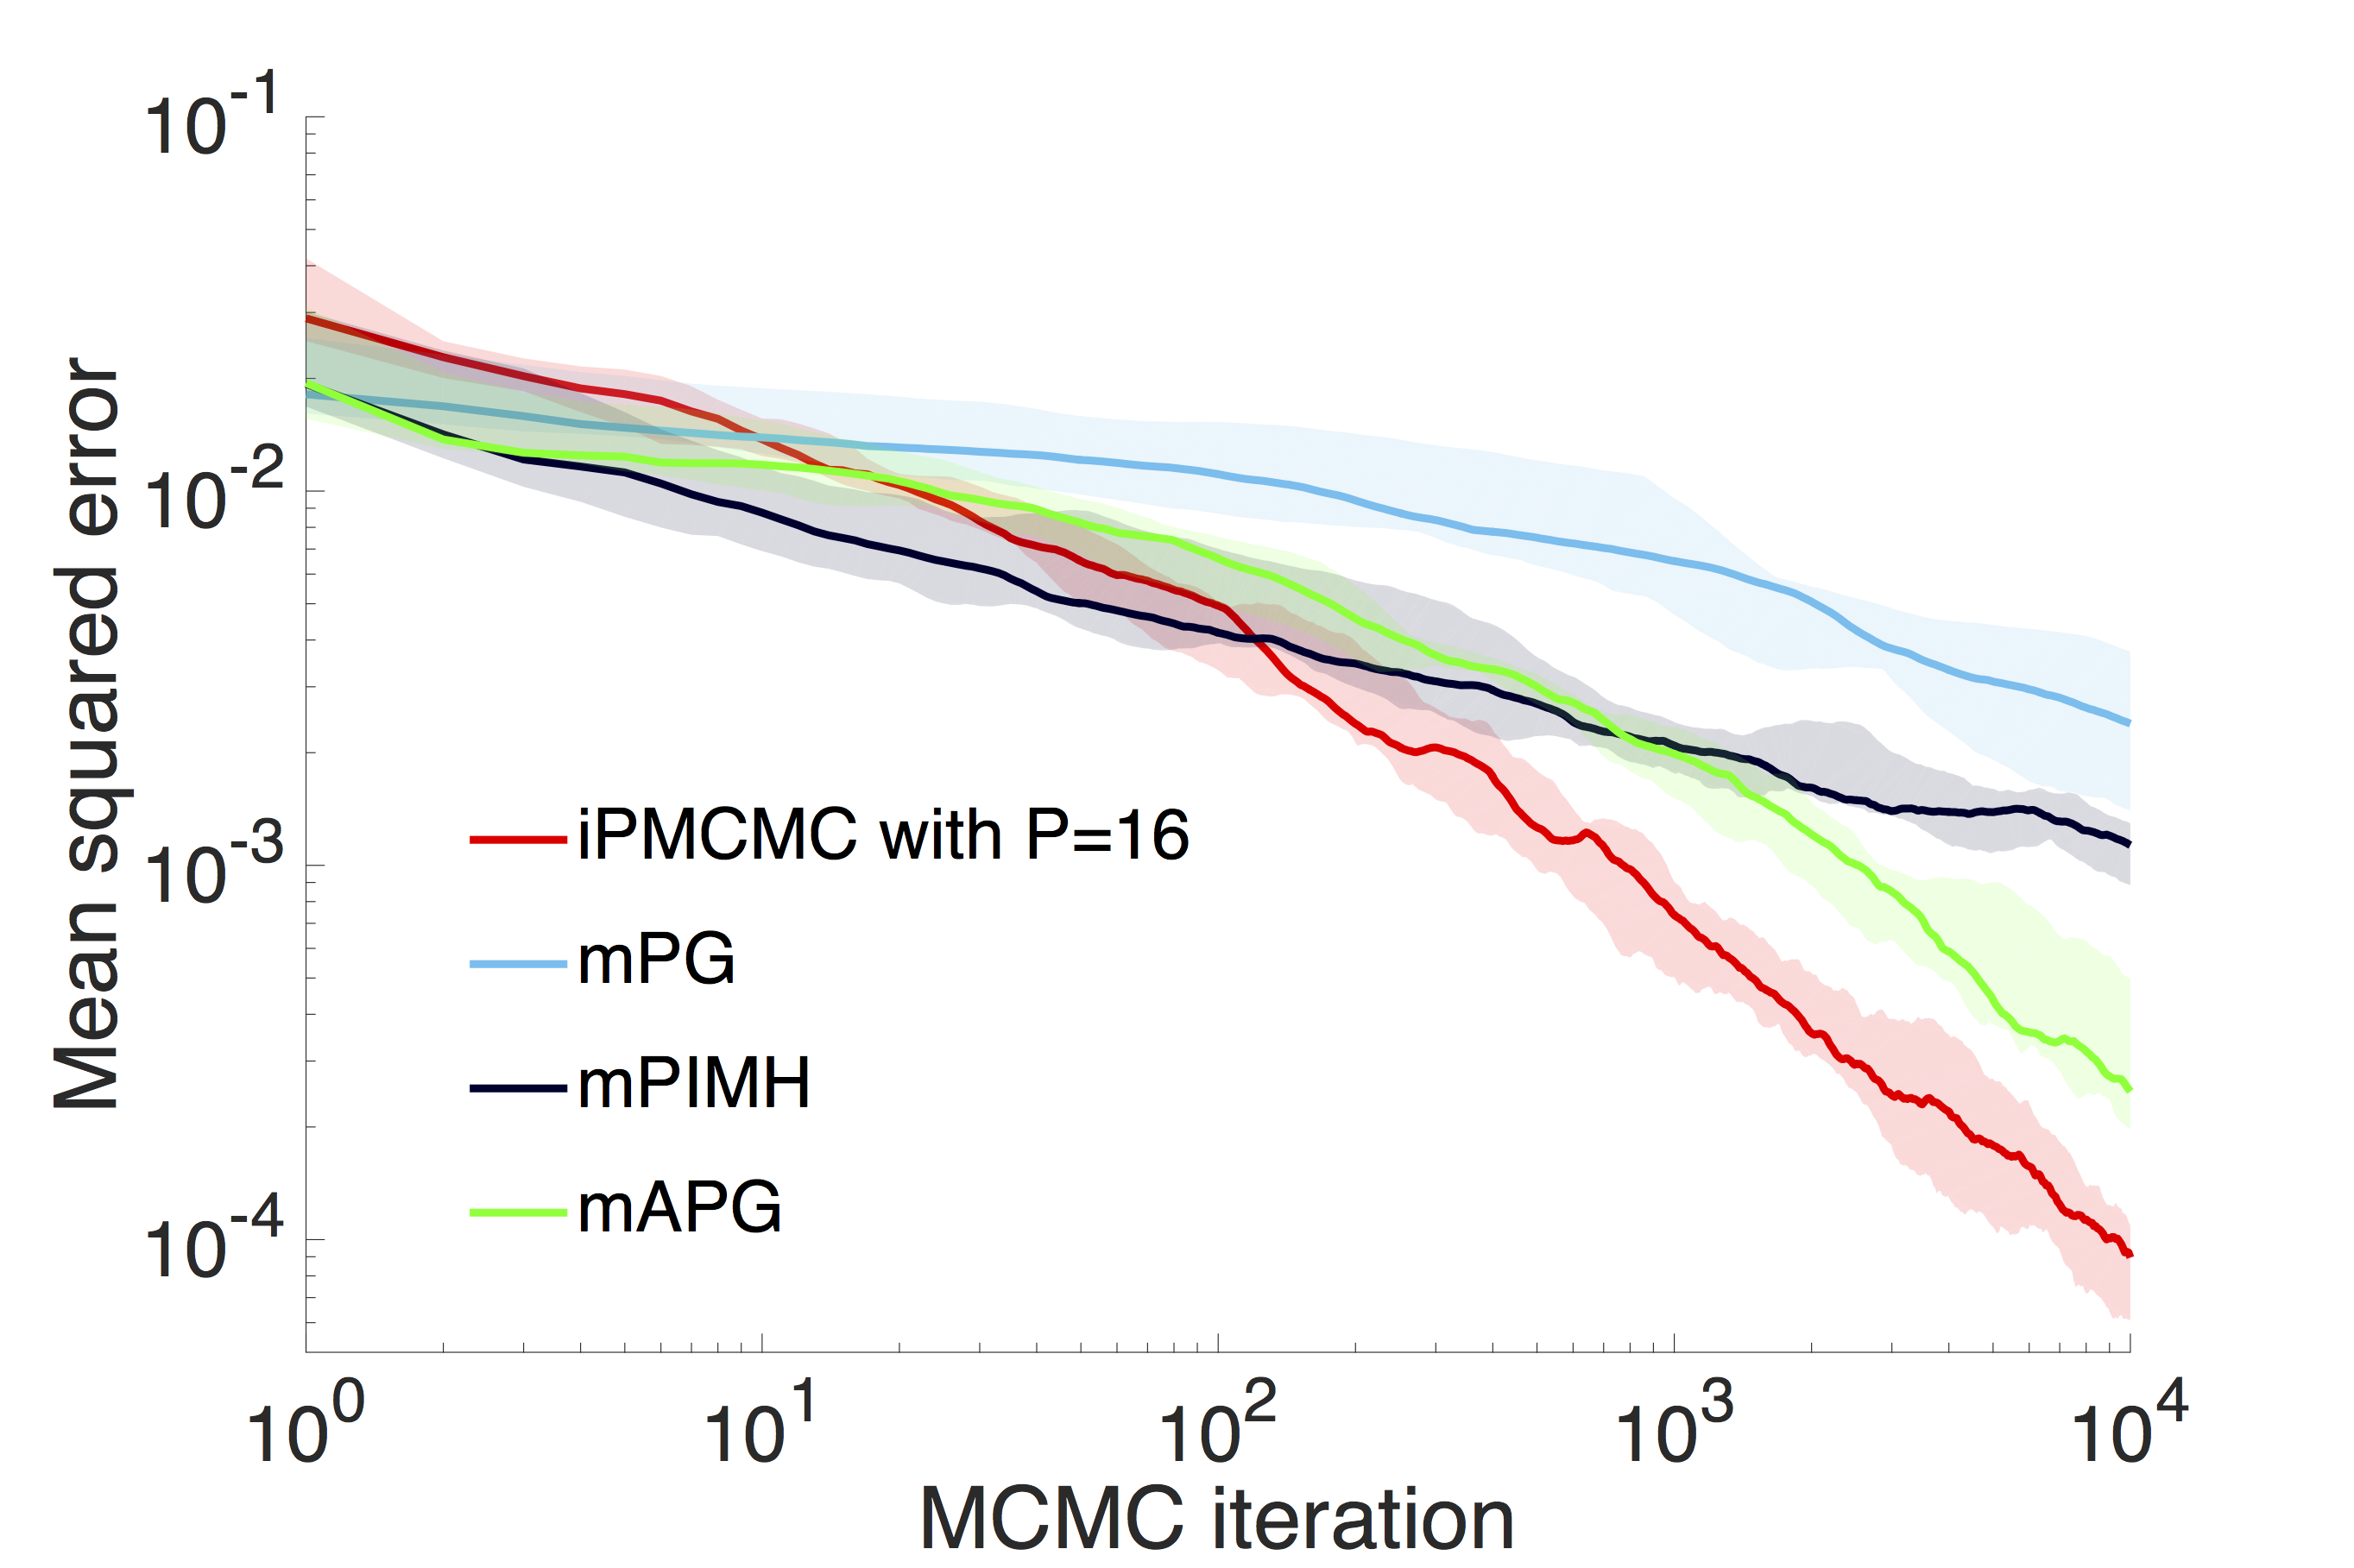
\includegraphics[width=\textwidth]{mean_conv_lss}
		\caption{Convergence in mean for full sequence}
		\label{fig:meanConv}
	\end{subfigure}
	~  %add desired spacing between images, e. g. ~, \quad, \qquad, \hfill etc. 
	%(or a blank line to force the subfigure onto a new line)
	\begin{subfigure}[t]{0.49\textwidth}
		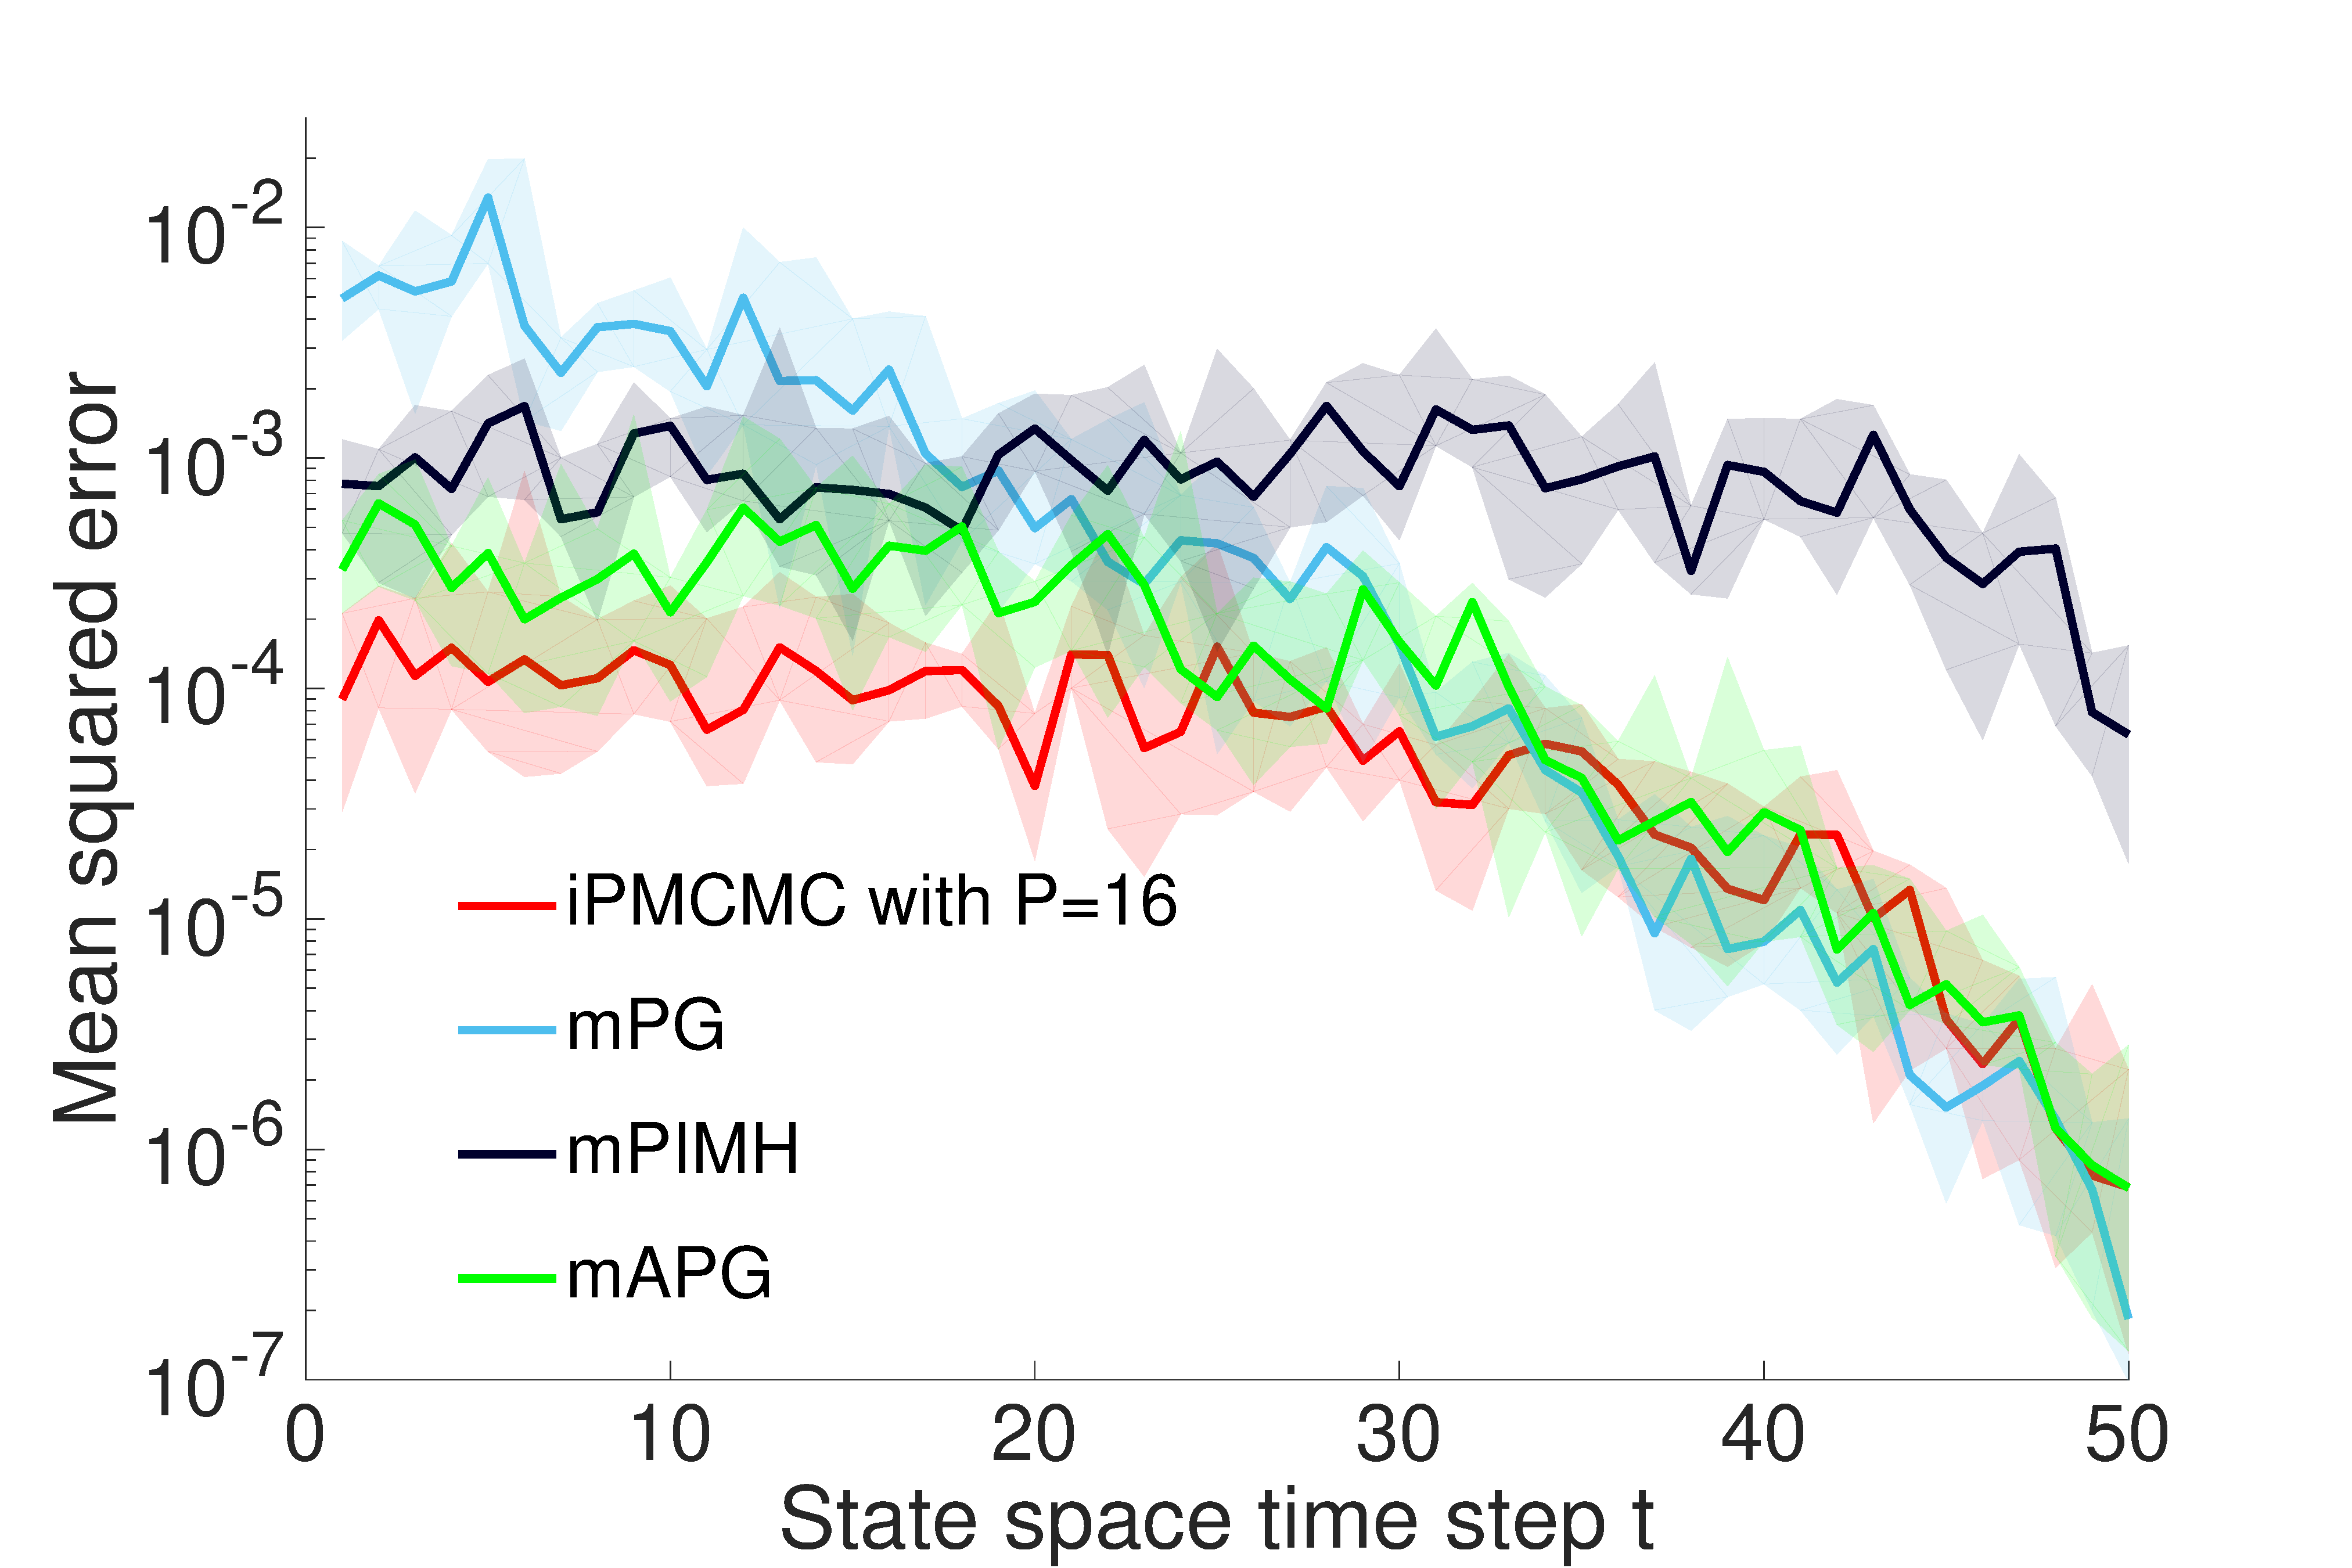
\includegraphics[width=\textwidth]{mean_pos_lss}
		\caption{Final error in mean for latent marginals}
		\label{fig:meanPos}
	\end{subfigure}
	
	%	\begin{subfigure}[t]{0.49\textwidth}
	%		\includegraphics[width=\textwidth]{std_conv_lss}
	%		\caption{Convergence in standard deviation for full sequence}
	%		\label{fig:stdConv}
	%	\end{subfigure}
	%	~ %add desired spacing between images, e. g. ~, \quad, \qquad, \hfill etc. 
	%	%(or a blank line to force the subfigure onto a new line)
	%	\begin{subfigure}[t]{0.49\textwidth}
	%		\includegraphics[width=\textwidth]{std_pos_lss}
	%		\caption{Final error in standard deviation for latent marginals}
	%		\label{fig:stdPos}
	%	\end{subfigure}	
	\caption{Mean squared error averaged over all dimensions and steps in the state sequence as a function of MCMC iterations (left) and mean squared error after $10^4$ iterations averaged over dimensions as function of position in the state sequence (right) for \eqref{eq:LGSS} with 50 time sequences.  The solid line shows the median error across the 10 tested synthetic datasets, while the shading shows the upper and lower quartiles.  Ground truth was calculated using the Rauch--Tung--Striebel smoother algorithm \cite{rauch1965maximum}. 
		\label{fig:groundTruth}}
\end{figure*}

\begin{figure*}[t]
	\centering
	\begin{subfigure}[t]{0.49\textwidth}
		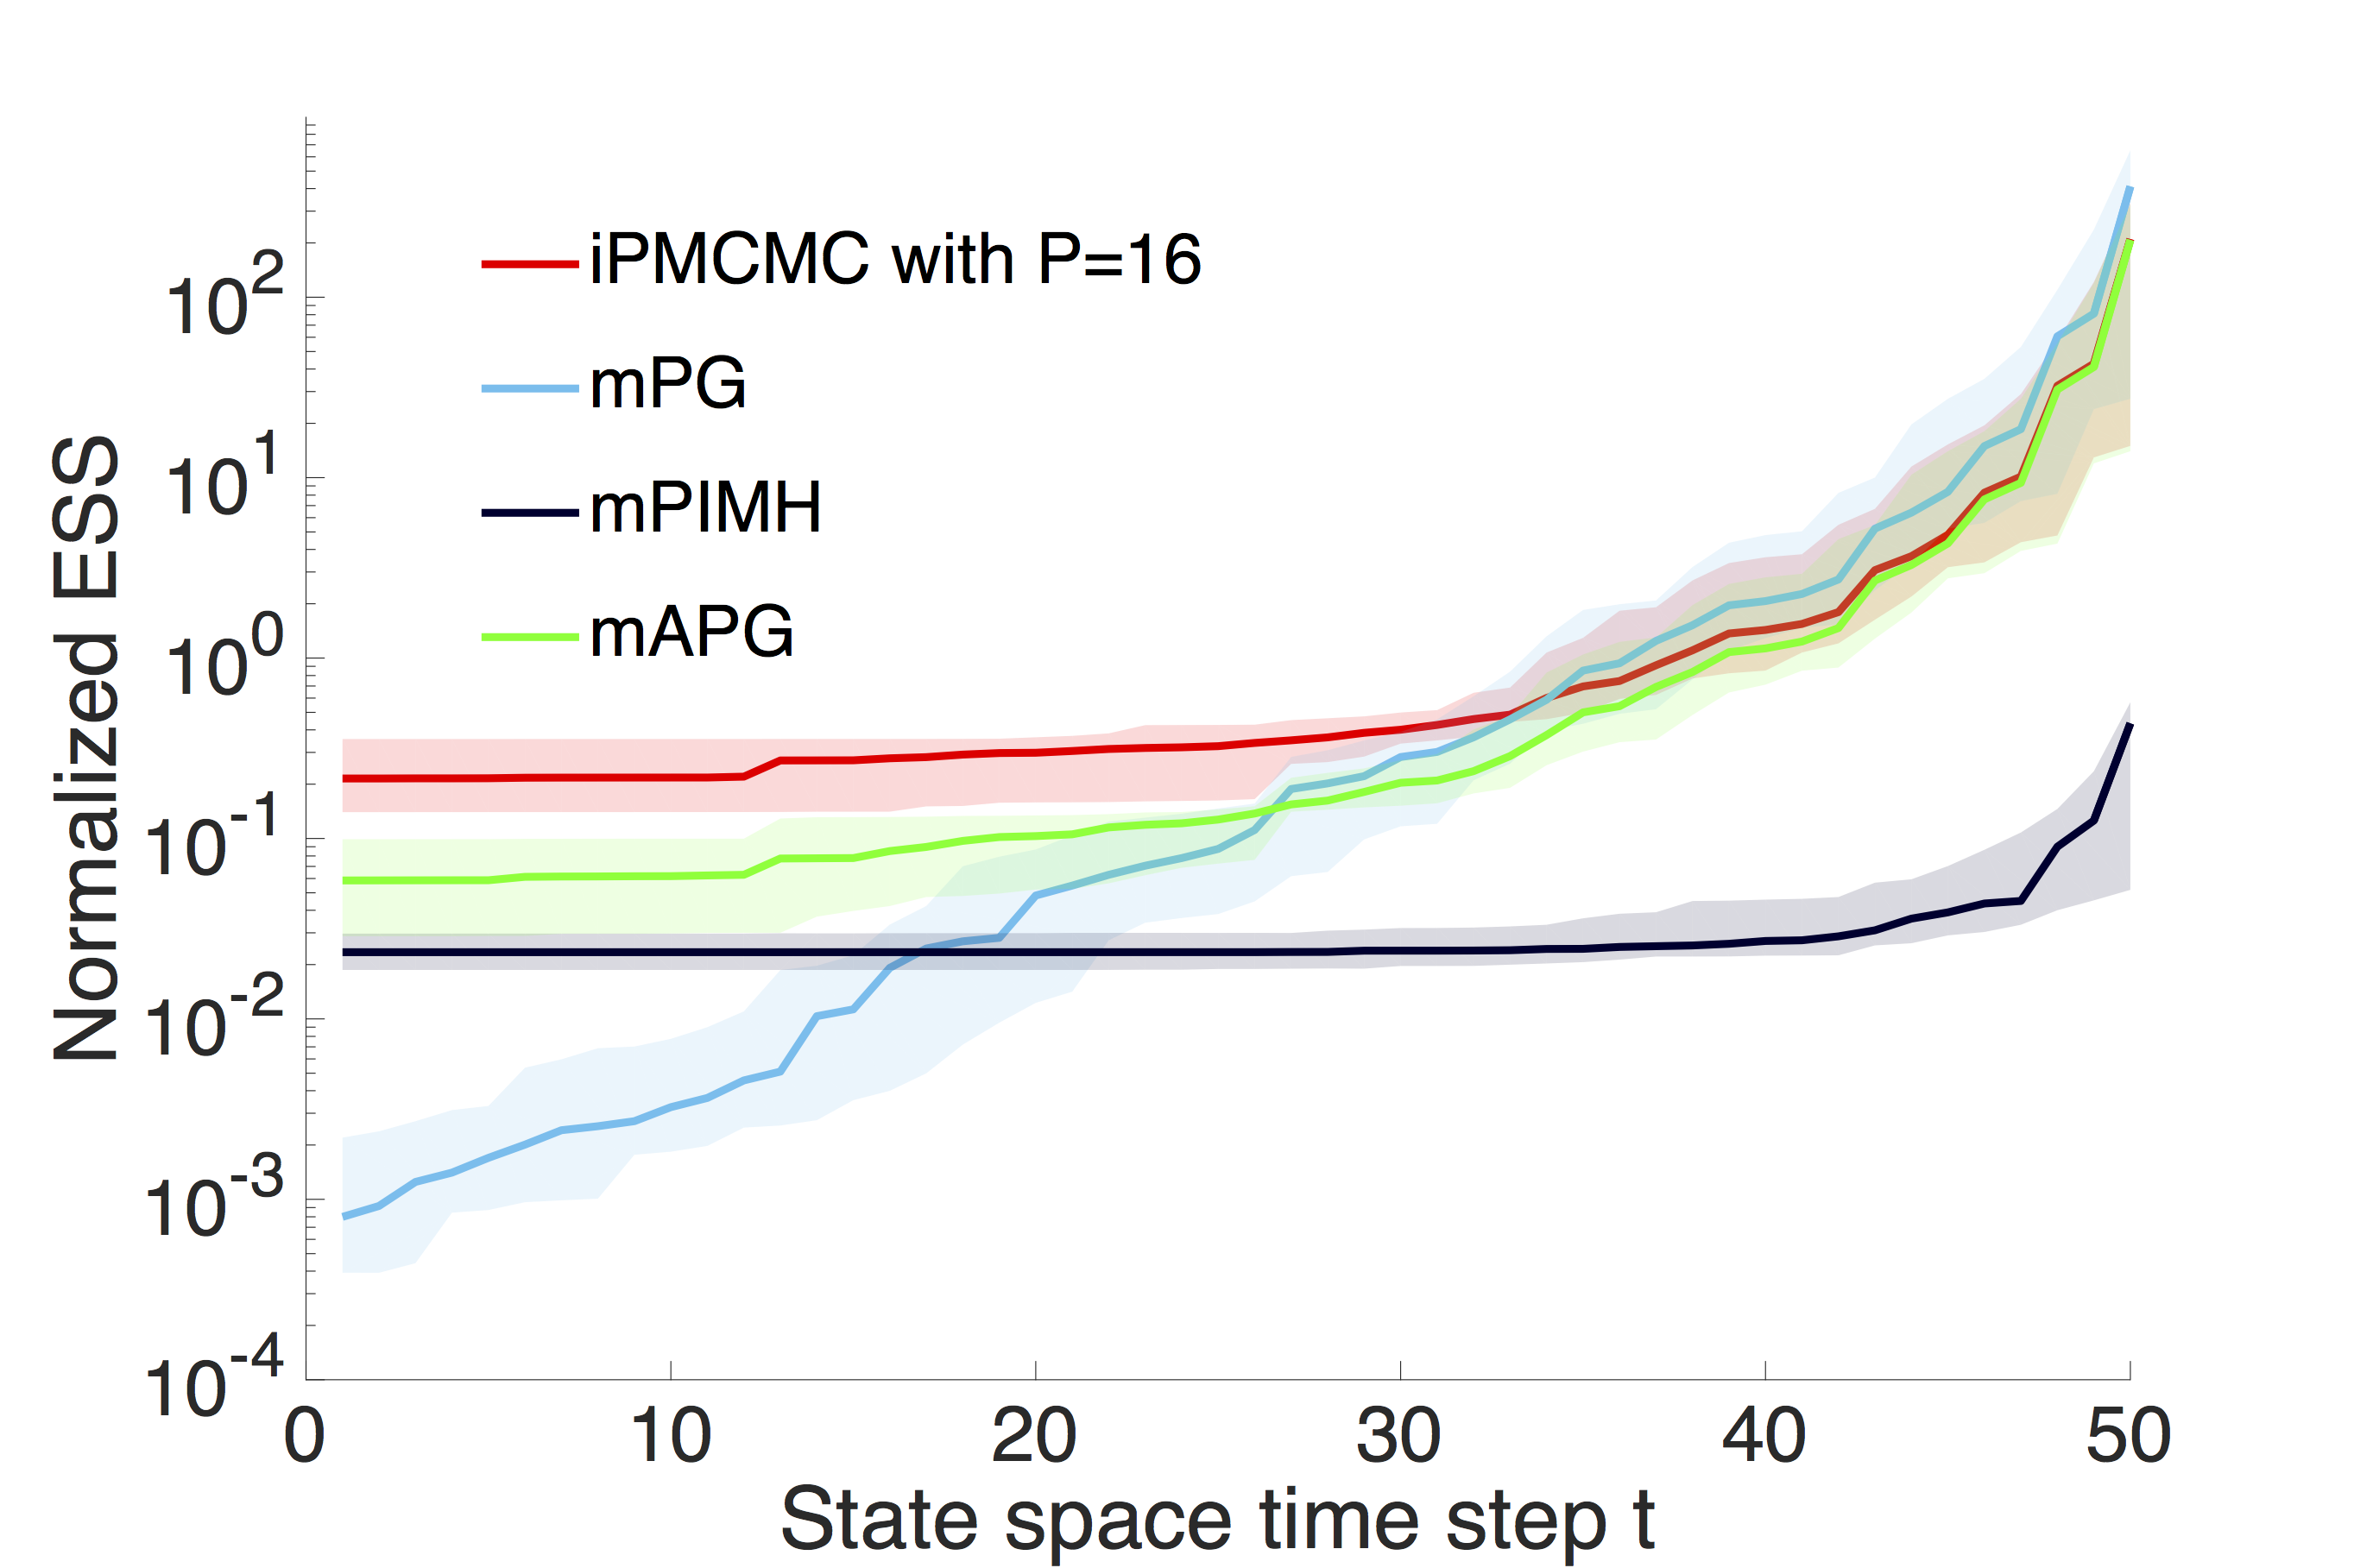
\includegraphics[width=\textwidth]{ess_lss}
		\caption{LGSSM}
	\end{subfigure}
	~ %add desired spacing between images, e. g. ~, \quad, \qquad, \hfill etc. 
	%(or a blank line to force the subfigure onto a new line)
	\begin{subfigure}[t]{0.49\textwidth}
		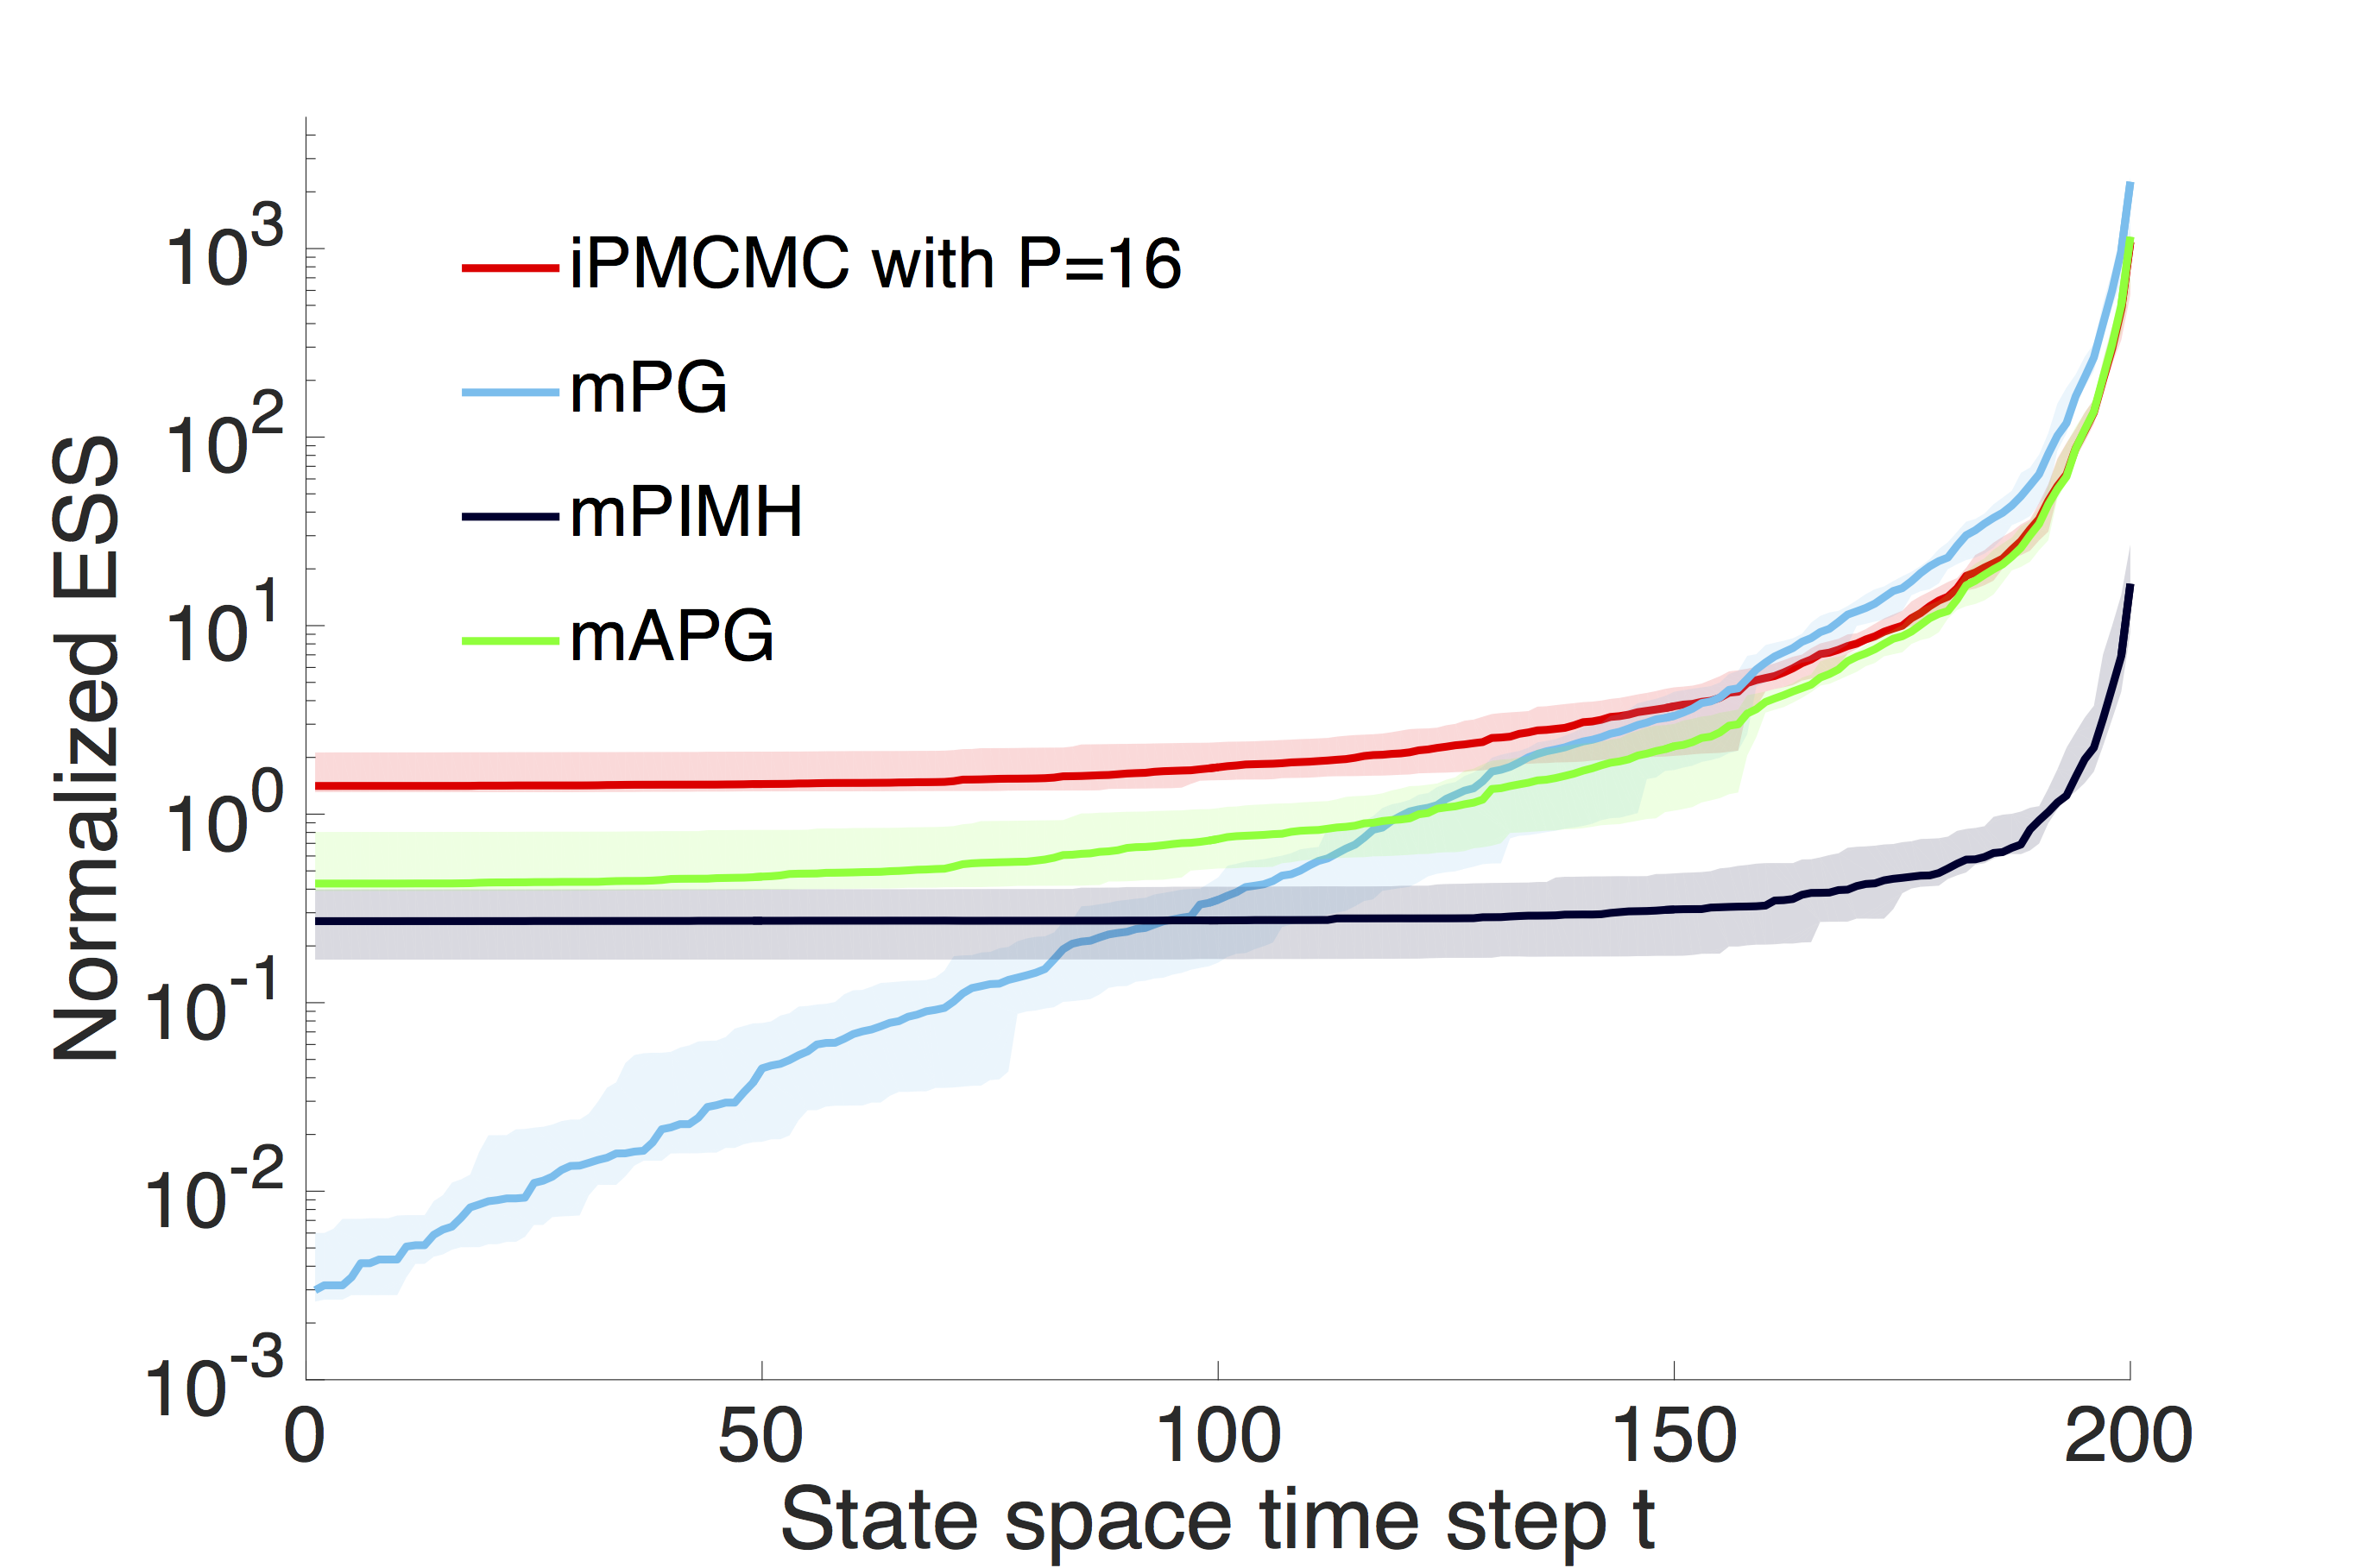
\includegraphics[width=\textwidth]{ess_nlss}
		\caption{NLSSM}
	\end{subfigure}
	
	\caption{Normalized effective sample size  (NESS) for LGSSM (left) and NLSSM (right).
		\label{fig:ESS}}
\end{figure*}

\subsubsection{Nonlinear State Space Model}
\label{sec:nlss}

We next consider the one dimensional nonlinear state space model (NLSSM) considered by, among others, \citet{gordon1993novel,andrieuDH2010}
\begin{subequations}
	\label{eq:NLSS}
	\begin{align}
	x_1 & \sim \mathcal{N} \left(\mu, v^2\right) \label{eq:NLSSa}\\
	x_t & = \frac{x_{t-1}}{2} + 25 \frac{x_{t-1}}{1+x_{t-1}^2} + 8 \cos \left(1.2t\right) + \delta_{t-1} \label{eq:NLSSb} \\
	y_t & = \frac{{x_{t}}^2}{20} + \varepsilon_{t} \label{eq:NLSSc}
	\end{align}
\end{subequations}
where $\delta_{t-1} \sim \mathcal{N} \left(0, \omega^2\right)$ and $\varepsilon_{t} \sim \mathcal{N} \left(0, \sigma^2\right)$.  We set the parameters as $\mu = 0$, $v=\sqrt{5}$, $\omega = \sqrt{10}$ and $\sigma = \sqrt{10}$.  Unlike the LGSSM, this model does not have an analytic solution and therefore one must resort to approximate inference methods. 
% such as sampling.
Further, the multi-modal nature of the latent space makes full posterior inference over $x_{1:T}$ challenging for long state sequences. 

\begin{figure*}[t]
	\centering
	%\begin{subfigure}[t]{0.99\textwidth}
	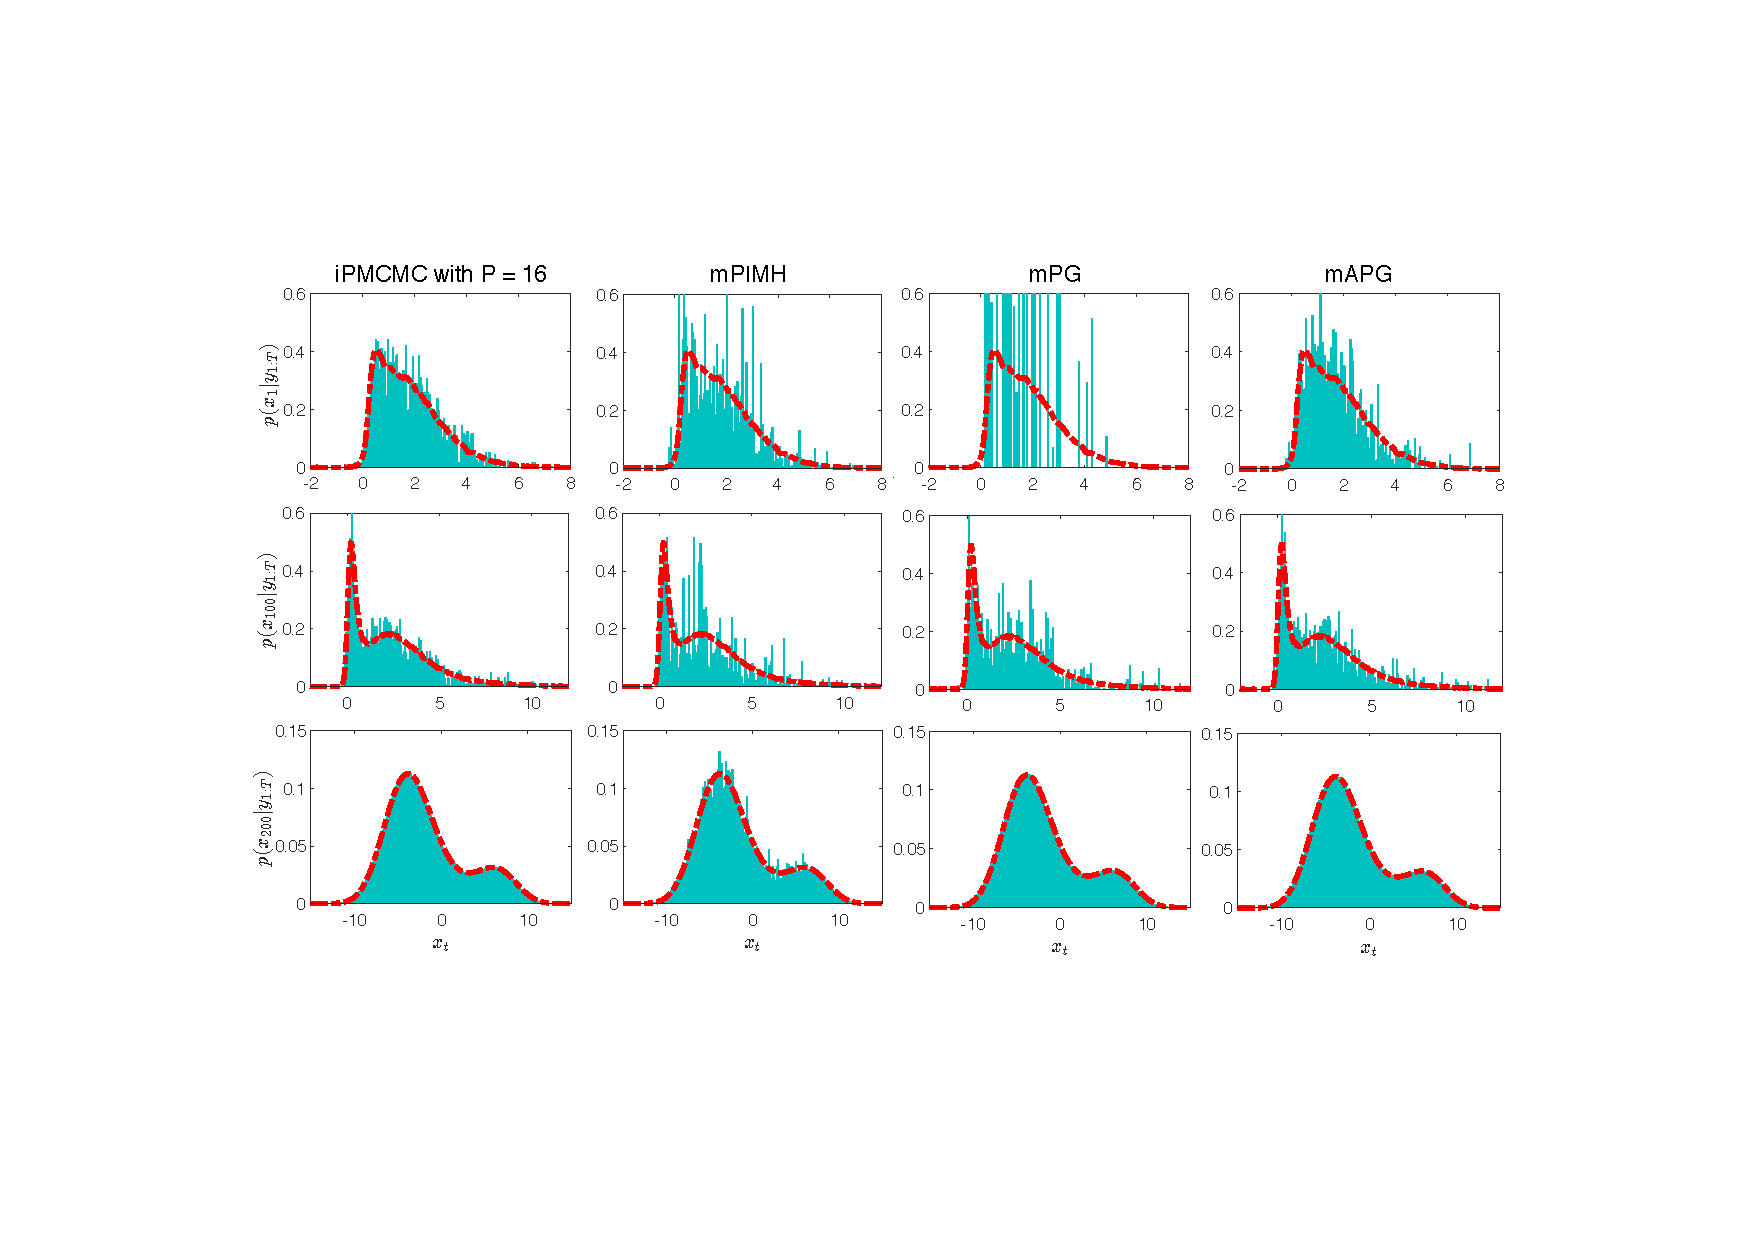
\includegraphics[width=1\textwidth]{nlss_histograms_minus_190.pdf}
	%\end{subfigure}
	\caption{Histograms of generated samples at $t=1, 100, \text{ and } 200$ for a single dataset generated from \eqref{eq:NLSS} with $T=200$.  Dashed red line shows an approximate estimate of the ground truth, found by running a kernel density estimator on the combined samples from a small number of independent SMC sweeps, each with $10^7$ particles. \label{fig:nlssHists}}
\end{figure*}

To examine the relative mixing of iPMCMC we calculate an effective sample size (ESS) for different steps in the state sequence.  In order to calculate the ESS, we condensed identical samples as done in for example \cite{vandemeent_aistats_2015}.  Let 
\begin{align*}
u_{t}^k \in \{x_{t,m}^{i}[r]\}^{i=1:N,r=1:R}_{m=1:M}, \quad \forall k \in 1 \dots K, \; t \in 1 \dots T
\end{align*} 
denote the unique samples of $x_t$ generated by all the nodes and sweeps of particular algorithm after $R$ iterations, where $K$ is the total number of unique samples generated.  The weight assigned to these unique samples, $v_t^{k}$, is given by the combined weights of all particles for which $x_t$ takes the value $u_{t}^k$:
\begin{align}
v_t^{k} = \sum_{r=1}^{R} \sum_{m=1}^{M} \sum_{i=1}^{N} \bar{w}_{t,m}^{i,r} \eta_{m}^{r} \delta_{x_{t,m}^{i}[r]}(u_{t}^{k})
\end{align}
where $\delta_{x_{t,m}^{i}[r]}(u_{t}^{k})$ is the Kronecker delta function and $\eta_{m}^{r}$ is a node weight.  For iPMCMC the node weight is given by as per the Rao-Blackwellized estimator described in Section~\ref{sec:allparticles}. For mPG and mPIMH, $\eta_{m}^{r}$ is simply $\frac{1}{RM}$,
as samples from the different nodes are weighted equally in the absence of interaction. 
Finally we define the effective sample size as $\text{ESS}_t = \left(\textstyle\sum_{k=1}^K \left(v_t^{k}\right)^2\right)^{-1}$.
%\begin{align}
%\label{eq:ESS}
%\text{ESS}_t = \left(\textstyle\sum_{k=1}^K \left(v_t^{k}\right)^2\right)^{-1}.
%\end{align}

Figure \ref{fig:ESS} shows the ESS for the LGSSM and NLSSM as a function of position in the state sequence.  For this, we omit the samples generated by the initialization step as this SMC sweep is common to all the tested algorithms.  We further normalize by the number of MCMC iterations so as to give an idea of the rate at which unique samples are generated.  These show that for both models the ESS of iPMCMC, mPG and mAPG is similar towards the end of the space sequence, but that iPMCMC outperforms all the other methods at the early stages. The ESS of mPG was particularly poor at early iterations.  PIMH performed poorly throughout, reflecting the very low observed acceptance ratio of around $7.3\%$ on average. 
%The lack of Monte Carlo convergence rate appearing in Figure \ref{fig:meanConv} also suggests this acceptance ratio is yet to converge, with the value in the ergodic regime likely to be even lower.   

It should be noted that the ESS is not a direct measure of performance for these models.  For example, the equal weighting of nodes is likely to make the ESS artificially high for mPG, mPIMH and mAPG, when compared with methods such as iPMCMC that assign a weighting to the nodes at each iteration.  To acknowledge this, we also plot histograms for the marginal distributions of a number of different position in the state sequence as shown in Figure \ref{fig:nlssHists}.  These confirm that iPMCMC and mPG have similar performance at the latter state sequence steps, whilst iPMCMC is superior at the earlier stages, with mPG producing almost no more new samples than those from the initialization sweep due to the degeneracy.  The performance of PIMH was consistently worse than iPMCMC throughout the state sequence, with even the final step exhibiting noticeable noise.

%An important feature of the ESS is that it is equal to the total number of samples ($NRM$) if all the samples are unique and have the same weight, and is equal to $1$ if there is only single unique sample with non-zero weight. It should be noted that ESS is not a direct measure of performance in the context of distributed PMCMC methods. In particular it takes no account of the suitability of the weights assigned to samples, for example the equal weighting assigned to different chains for mPG and mPIMH mean they will always have a higher ESS for a particle sweep \brooks{clarify ``particle sweep''?} than a iPMCMC sweep generating the same samples, regardless of whether this equal weighting gives a better approximation to the true posterior. \fredrik{I did not quite understand the last sentence.}


\section{Discussion and Future Work}
\label{sec:disc}

% !TEX root = ../main.tex

\chapter{Challenges, Criticisms, and Future Directions}
\label{chp:discussion}

\newpage

\appendix

\section{Program Transformations in Detail}
\label{sec:program-transformations}
% !TEX root = ../main.tex

In this section we give a more detailed and language specific description of our program transformations, code for which can be found at \href{http://www.github.com/probprog/bopp}{\url{http://www.github.com/probprog/bopp}}. %We will refer to the code in explaining the implementation of program transformations for BOPP.

\subsection{Anglican}
Anglican is a probabilistic programming language integrated into Clojure (a dialect of Lisp) and inherits most of the corresponding syntax. Anglican extends Clojure with the special forms \sample and \observe \citep{tolpin2015probabilistic}.  
Each random draw in an Anglican program corresponds to a \sample  call, which can be thought of as a term in the prior. 
Each \observe statement applies weighting to a program trace and thus constitutes a term in the likelihood.
Compilation of an Anglican program, performed by the macro \lsi{query}, corresponds to transforming the code into a variant of continuation-passing style (CPS) code, which results in a function that can be executed using a particular inference algorithm.

Anglican program code is represented by a nested list of expressions, symbols, non-literals for contructing data structures (e.g. \lsi{[...]} for vectors), and command dependent literals (e.g. \lsi{[...]} as a second argument of a \lsi{let} statement which is used for binding pairs).  In order to perform program transformations, we can recursively traverse this nested list which can be thought of as an abstract syntax tree of the program.

Our program transformations also make use of the Anglican forms \lsi{store} and \lsi{retrieve}.  These allow storing any variable in the probabilistic program's execution trace in a state which is passed around during execution and from which we can retrieve these stored values.  The core use for this is to allow the outer query to return variables which are only locally scoped.

To allow for the early termination that will be introduced in Section \ref{sec:bopp-supp/early-term}, it was necessary to add a mechanism for non-local returns to Anglican.  Clojure supports non-local returns only through Java exception handling, via the keywords {\bf\ttfamily\color{cyan} try}~{\bf\ttfamily\color{cyan}throw},~{\bf\ttfamily\color{cyan}catch} and {\bf\ttfamily\color{cyan}finally}.  Unfortunately, these are not currently supported by Anglican and their behaviour is far from ideal for our purposes.  In particular, for programs containing nested {\bf\ttfamily\color{cyan}try} statements, throwing to a particular {\bf\ttfamily\color{cyan}try} in the stack, as opposed to the most recently invoked, is cumbersome and error prone.
%
%Firstly, return values are stored within exceptions which is cumbersome and can cause issues in debugging.  Secondly, it is difficult to control the point of return.  For example, imagine we wish to return from the query itself and so wrap the original query in a {\bf\ttfamily\color{cyan}try-catch} block.  Na\"{i}vely throwing might now cause us to return to an unexpected point if the original query already contained a {\bf\ttfamily\color{cyan}try-catch} block.  Thus controlling the exact return point would require a careful and error-prone mechanism based on custom exception types and catches.

We have instead, therefore, added to Anglican a non-local return mechanism based on the Common Lisp control form \lsi{catch/throw}.  This uses a \emph{catch tag} to link each \lsi{throw} to a particular \lsi{catch}.  For example
\begin{lstlisting}[basicstyle=\footnotesize\ttfamily]
(catch :tag
  (when (> a 0)
    (throw :tag a))
  0)
\end{lstlisting}
is equivalent to \lsi{(max a 0)}.  More precisely, \lsi{throw} has syntax \lsi{(throw tag value)} and will cause the \lsi{catch} block with the corresponding \lsi{tag} to exit, returning \lsi{value}.   If a \lsi{throw} goes uncaught, i.e. it is not contained within a \lsi{catch} block with a matching tag, a custom Clojure exception is thrown.

%To allow for the early termination discussed in Section \ref{sec:bopp-supp/early-term}, it was necessary to add one new primitive to Anglican, namely \lsi{return} with syntax \lsi{(return return-val)}.  At a high level, \lsi{return} causes the query to terminate, returning \lsi{return-val}.  This is done by, during runtime of the CPS compiled code, returning a Clojure record \lsi{->result} containing \lsi{return-val} instead of a valid program continuation, causing the query execution to terminate and return the required value.

\subsection{Representations in the Main Paper}
\label{sec:bopp-supp/main-paper-rep}

In the main paper we presented the code transformations as static transformations as shown in Figure~\ref{fig:bopp_overview}.  Although for simple programs, such as the given example, these transformations can be easily expressed as static transformations, for more complicated programs it would be difficult to actually implement these as purely static generic transformations in a higher-order language.  Therefore, even though all the transformations dynamically execute as shown at runtime, in truth, the generated source code for the prior and acquisition transformations varies from what is shown and has been presented this way in the interest of exposition.  Our true transformations exploit \lsi{store}, \lsi{retrieve}, \lsi{catch} and \lsi{throw} to generate programs that dynamically execute in the same way at run time as the static examples shown, but whose actual source code varies significantly.

\subsection{Prior Transformation}
\label{sec:bopp-supp/prior-transformations}
The prior transformation recursively traverses the program tree and applies two local transformations.  
Firstly it replaces all \observe statements by \lsi{nil}.  
As \observe statements return \lsi{nil}, this trivially preserves the generative model of the program, but the probability of the execution changes. 
Secondly, it inspects the binding variables of \lsi{let} forms in order to modify the binding expressions for the optimization variables, as specified by the second input of \defopt, asserting that these are directly bound to a \sample statement of the form \texttt{(\sample dist)}.
The transformation then replaces this expression by one that stores the result of this sample in Anglican's \lsi{store} before returning it.
Specifically, if the binding variable in question is \lsi{phi-}$\ell$, then the original binding expression \lsi{(sample dist)} is transformed into
% \begin{figure}
    \begin{lstlisting}[basicstyle=\footnotesize\ttfamily]
(let [value (sample dist)]
  ;; Store the sampled value in Anglican's store
  (store OPTIM-ARGS-KEY
         'phi-$\ell$
         value)
  value)
    \end{lstlisting}
%     \caption{}
%     \label{fig:prior-1}
% \end{figure}

After all these local transformation have been made, we wrap the resulting query block in a \lsi{do} form and append an expression extracting the optimization variables using Anglican's \lsi{retrieve}.  This makes the optimization variables the output of the query.  Denoting the list of optimization variable symbols from \defopt as \lsi{optim-args} and the query body after applying all the above location transformations as \dots, the prior query becomes
% \begin{figure}
    \begin{lstlisting}[basicstyle=\footnotesize\ttfamily]
(query query-args
  (do
    ...
    (map (fn [x] (retrieve OPTIM-ARGS-KEY x))
       optim-args)))
    \end{lstlisting}
%     \caption{}
%     \label{fig:prior-3}
% \end{figure}
Note that the difference in syntax from Figure~\ref{fig:bopp_overview} is because \lsi{defquery} is in truth a syntactic sugar allowing users to bind \lsi{query} to a variable.  As previously stated, \lsi{query} is macro that compiles an Anglican program to its CPS transformation.  An important subtlety here is that the order of the returned samples is dictated by \lsi{optim-args} and is thus independent of the order in which the variables were actually sampled, ensuring consistent inputs for the BO package.

We additionally add a check (not shown) to ensure that all the optimization variables have been added to the store, and thus sampled during the execution, before returning.  This ensures that our assumption that each optimization variable is assigned for each execution trace is satisfied.

\subsection{Acquisition Transformation}
\label{sec:bopp-supp/acq-transformations}
The acquisition transformation is the same as the prior transformation except we append the acquisition function, \lsi{ACQ-F}, to the inputs and then \observe its application to the optimization variables before returning.
The acquisition query is thus
% \begin{figure}
    \begin{lstlisting}[basicstyle=\footnotesize\ttfamily]
(query [query-args ACQ-F]
  (do
    ...
    (let [theta (map (fn [x] (retrieve OPTIM-ARGS-KEY x))
                      optim-args)]
      (observe (factor) (ACQ-F theta))
      theta)))
    \end{lstlisting}
%     \caption{}
%     \label{fig:acq-1}
% \end{figure}

\subsection{Early Termination}
\label{sec:bopp-supp/early-term}
To ensure that \lsi{q-prior} and \lsi{q-acq} are cheap to evaluate and that the latter does not include unnecessary terms which complicate the optimization, we wish to avoid executing code that is not required for generating the optimization variables.
Ideally we would like to directly remove all such redundant code during the transformations.
However, doing so in a generic way applicable to all possible programs in a higher order language represents a significant challenge.
Therefore, we instead transform to programs with additional early termination statements, triggered when all the optimization variables have been sampled.  
Provided one is careful to define the optimization variables as early as possible in the program (in most applications, e.g. hyperparameter optimization, they naturally occur at the start of the program), this is typically sufficient to ensure that the minimum possible code is run in practise.

To carry out this early termination, we first wrap the query in a \lsi{catch} block with a uniquely generated tag.  We then augment the transformation of an optimization variable's binding described in Section~\ref{sec:bopp-supp/prior-transformations} to check if all optimization variables are already stored, and invoke a \lsi{throw} statement with the corresponding tag if so.  Specifically we replace relevant binding expressions \lsi{(sample dist)} with
% \begin{figure}
    \begin{lstlisting}[basicstyle=\footnotesize\ttfamily]
(let [value (sample dist)]
  ;; Store the sampled value in Anglican's store
  (store OPTIM-ARGS-KEY
         'phi-$\ell$
         value)
  ;; Terminate early if all optimization variables are sampled
  (if (= (set (keys (retrieve OPTIM-ARGS-KEY)))
         (set optim-args))
    (throw BOPP-CATCH-TAG prologue-code)
    value))
    \end{lstlisting}
%     \caption{}
%     \label{fig:early-termination}
% \end{figure}
where \lsi{prologue-code} refers to one of the following expressions depending on whether it is used for a prior or an acquisition transformation
% \begin{figure}
    \begin{lstlisting}[basicstyle=\footnotesize\ttfamily]
;; Prior query prologue-code
(map (fn [x] (retrieve OPTIM-ARGS-KEY x))
             optim-args)

;; Acquisition query prologue-code
(do
  (let [theta (map (fn [x] (retrieve OPTIM-ARGS-KEY x))
                    optim-args)]
  (observe (factor) (ACQ-F theta))
  theta))
    \end{lstlisting}
%     \caption{}
%     \label{fig:early-termination-2}
% \end{figure}

We note that valid programs for both \lsi{q-prior} and \lsi{q-acq} should always terminate via one of these early stopping criteria and therefore never actually reach the appending statements in the \lsi{query} blocks shown in Sections \ref{sec:bopp-supp/prior-transformations} and \ref{sec:bopp-supp/acq-transformations}.  As such, these are, in practise, only for exposition and error catching.

\subsection{Marginal/MMAP Transformation}
The marginal transformation inspects all \lsi{let} binding pairs and if a binding variable \lsi{phi-}$\ell$ is one of the optimization variables, the binding expression \lsi{(sample dist)} is transformed to the following
% \begin{figure}
    \begin{lstlisting}[basicstyle=\footnotesize\ttfamily]
(do (observe dist phi-$\ell$-hat)
    phi-$\ell$-hat)
    \end{lstlisting}
%     \caption{}
%     \label{fig:marg-1}
% \end{figure}
corresponding to the \lsi{observe<-} form used in the main paper.

\subsection{Error Handling}
\label{sec:bopp:trans:error}
During program transformation stage, we provide three error-handling mechanisms to enforce the restrictions on the probabilistic programs described in Section~\ref{sec:problem}.
\begin{enumerate}
    \item We inspect \lsi{let} binding pairs and throw an error if an optimization variable is bound to anything other than a \sample statement.
    \item We add code that throws a runtime error if any optimization variable is assigned more than once or not at all.
    \item We recursively traverse the code and throw a compilation error if \sample statements of different base measures are assigned to any optimization variable.  At present, we also throw an error if the base measure assigned to an optimization variable is unknown, e.g. because the distribution object is from a user defined \lsi{defdist} where the user does not provide the required measure type meta-information.
\end{enumerate}


\section{Problem Independent Gaussian Process Hyperprior}
\label{sec:app:hyperprior}

% !TEX root = bopp.tex

Remembering that the domain scaling introduced in Section~\ref{sec:domain} means that both the input and outputs of the GP are taken to vary between $\pm1$, we define the problem independent GP hyperprior as $p(\alpha)=p(\sigma_n)p(\sigma_{3/2})p(\sigma_{5/2})\prod_{i=1}^{D}p(\rho_i)p(\varrho_i)$ where
\begin{subequations}
	\begin{align}
	\label{eq:hyperPriorDef}
	\log \left(\sigma_n\right) & \sim \mathcal{N} \left(-5,2\right) \\
	\log\left(\sigma_{3/2}\right) & \sim \mathcal{N} \left(-7,0.5\right)\\
	\log\left(\sigma_{5/2}\right) & \sim \mathcal{N} \left(-0.5,0.15\right)\\
	\log \left(\rho_i\right) & \sim \mathcal{N} (-1.5,0.5) \quad \forall i \in \{1,\dots,D\}\\
	\log\left(\varrho_i\right) & \sim \mathcal{N} \left(-1,0.5\right) \quad \forall i \in \{1,\dots,D\}.
	\end{align}
\end{subequations}
The rationale of this hyperprior is that the smoother Mat\'{e}rn 5/2 kernel should be the dominant effect and model the higher length scale variations. The Mat\'{e}rn 3/2 kernel is included in case the evidence suggests that the target is less smooth than can be modelled with the Mat\'{e}rn 5/2 kernel and to provide modelling of smaller scale variations around the optimum.

\section{Full Details for House Heating Experiment}
\label{sec:app:heating}

% !TEX root =  bopp.tex

In this case study, illustrated in Figure~\ref{fig:houses}, we optimize the parameters of a stochastic engineering simulation. We use the Energy2D system from \cite{xie2012energy2d} to perform finite-difference numerical simulation of the heat equation and Navier-Stokes equations in a user-defined geometry. 

In our setup, we designed a 2-dimensional representation of a house with 4 interconnected rooms using the GUI provided by Energy2D. The left side of the house receives morning sun, modelled at a constant incident angle of $30^\circ$. We assume a randomly distributed solar intensity and simulate the heating of a cold house in the morning by 4 radiators, one in each of the rooms. The radiators are given a fixed budget of total power density $P_{\text{budget}}$. The optimization problem is to distribute this power budget across radiators in a manner that minimizes the variance in temperatures across 8 locations in the house. 

Energy2D is written in Java, which allows the simulation to be integrated directly into an Anglican program that defines a prior on model parameters and an ABC likelihood for evaluating the utility of the simulation outputs. Figure \ref{fig:house-heating-code} shows the corresponding program query. In this, we define a Clojure function \lsi{simulate} that accepts a solar power intensity $I_{\text{sun}}$ and power densities for the radiators $P_{\text{r}}$, returning the thermometer temperature readings $\{T_{i, t}\}$. We place a symmetric Dirichlet prior on $\frac{P_r}{P_{\text{budget}}}$ and a gamma prior on $\frac{I_{\text{sun}}}{I_{base}}$, where $P_{\text{budget}}$ and $I_{base}$ are constants. This gives the generative model:
 \begin{align}
 p_r &\sim \Dirichlet([1,1,1,1]) \\
 P_r &\leftarrow P_{\text{budget}} \cdot p_r \\
 \upsilon &\sim \text{Gamma}(5,1) \\
 I_{\text{sun}} &\leftarrow I_{\text{base}} \cdot \upsilon.
 \end{align}
After using these to call \lsi{simulate}, the standard deviations of the returned temperatures is calculated for each time point,
\begin{align}
\omega_t = \sqrt{\sum_{i=1}^8 T_{i, t}^2 -\left(\sum_{i=1}^8 T_{i, t}\right)^2}
\end{align}
and used in the ABC likelihood \lsi{abc-likelihood} to weight the execution trace using a multivariate Gaussian:
\begin{align*}
p\left(\{T_{i, t}\}_{i = 1:8, t = 1:\tau}\right) = \text{Normal}\left(\omega_{t=1:\tau};\mathbf{0},\sigma_T^{2}\mathbf{I}\right)
\end{align*}
where $\mathbf{I}$ is the identity matrix and $\sigma_T = 0.8 ^{\circ} \mathrm{C}$ is the observation standard deviation.

Figure \ref{fig:houses} demonstrates the improvement in homogeneity of temperatures as a function of total number of simulation evaluations. Visual inspection of the heat distributions also shown in Figure \ref{fig:houses} confirms this result, which serves as an exemplar of how BOPP can be used to estimate marginally optimal simulation parameters.


\newpage

\section*{Acknowledgements}
Tom Rainforth is supported by a BP industrial grant. Tuan Anh Le is supported by a Google studentship, project code DF6700.  Frank Wood is supported under DARPA PPAML through the U.S. AFRL under Cooperative Agreement FA8750-14-2-0006, Sub Award number 61160290-111668.

\bibliography{refsBOPP}{}

\end{document}
